% base document setting
\documentclass[a4,paper,12pt]{article}

% load packages
\usepackage{pkg/layout_print}
%\usepackage{pgfplots}
%\usepackage{pgfplotstable}
\usepackage{filecontents}
%\usepackage{pkg/pgf-pie}

% user defined macros

% load glossary entries
\newglossaryentry{} {
	name 		= {},
	description	= {}
}


	% glossary
\newacronym{pwm}{PWM}{Puslweitenmodulation}

\newacronym{psm}{PSM}{Phasenverschiebungsmodulation}

\newacronym{zvs}{ZVS}{Zero-Voltage Switching}

\newacronym{zcs}{ZCS}{Zero-Current Switching}

\newacronym{psm_ppc}{PSM Wandler}{Gegentaktwandler mit Phasenverschiebungsmodulation}

\newacronym{pwm_ppc}{PWM Wandler}{Gegentaktwandler mit Pulsweitenmodulation}

\newacronym{wav}{WAV}{Waveform Daten}

\newacronym{mosfet}{MOSFET}{Metall-Oxid-Halbleiter Feldeffekttransistor (engl. \emph{metal-oxide-semicoductor field-effect transsitor})}

\newacronym{esr}{ESR}{äquivalente Seriewiderstand (engl. \emph{equivalent series resistance})}

\newacronym{soc}{SOC}{Ladezustand (engl. \emph{State-of-Charge})}

\newacronym{soh}{SOH}{Gesundheitszustand (engl. \emph{State-of-Health})}

\newacronym{bms}{BMS}{Batteriemanagementsystem}

\newacronym{ocv}{OCV}{Leerlaufspannung}

\newacronym{emf}{EMF}{elektromotorische Kraft (engl. \emph{electromotive force})}

\newacronym{cc}{CC}{Konstantstrom (engl. \emph{constant current})}

\newacronym{cv}{CV}{Konstantspannung (engl. \emph{constant voltage})}

\newacronym{sd}{SD}{Standardabweichung (engl. \emph{standard deviation})}

\newacronym{pkw}{PKW}{Personenkraftwagen}

\newacronym{lkw}{LKW}{Lastkraftwagen}

\newacronym{vrla}{VRLA}{ventilgeregelte Blei-Säure Batterie (engl. \emph{Valve Regulated Lead-Acid Battery})}

\newacronym{agm}{AGM}{absorbierende Glassmatte Batterie (engl. \emph{Absorbtive Glass Matt Battery})}

\newacronym{eis}{EIS}{elektrochemische Impedanzspektroskopie (engl. \emph{electrochemical impedance spectroscopy})}

\newacronym{ups}{UPS}{unterbrechungsfreie Stromversorgung (engl. \emph{uniterruptible power supply})}

\newacronym{esb}{ESB}{Ersatzschaltbild (engl. \emph{equivalent circuit})}
	% actronyms
\makeglossaries

\newcommand{\changefont}[3]{
	\fontfamily{#1} \fontseries{#2} \fontshape{#3} \selectfont
}

\newtoggle{printversion}		% definition for print or onlineversion
\toggletrue{printversion}		% uncomment for printversion
%\togglefalse{printversion}		% uncomment for onlineversion

\newtoggle{measurementdetails}		% definition for full measurement details or summary
%\toggletrue{measurementdetails}	% uncomment for full details
\togglefalse{measurementdetails}	% uncomment for summary

% document
\begin{document}

	% change font
	%\changefont{phv}{m}{n}		% helvetica
	%\changefont{cmtt}{m}{sl}	% computer modern typewriter
	%\changefont{cmss}{m}{n}	% computer modern sans serif

	% input contents
	% titlepages
\begin{titlepage}
	\centering
	% left bottom right top
%	\includegraphics[trim = 20mm 100mm 20mm 20mm, clip, width = 50mm]{pic/title.jpg}\par\vspace{1cm} \nocite{wr}
	
	{\scshape\LARGE Hochschule Luzern \par}
	\vspace{0.75cm}
	{\scshape\Large EMANT Laborbericht 1\par}
	\vspace{1cm}
	{\huge\bfseries Monopol Antenne\par}
	\vspace{1.5cm}
	{\Large\itshape Markus Birrer\par}
	\vspace{0.5cm}
	
	\begin{figure}[htbp]
		\centering
		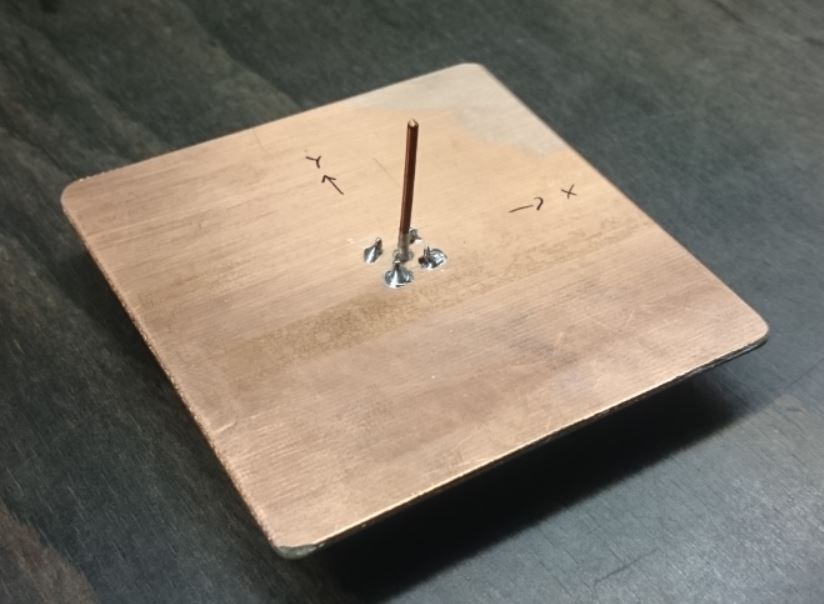
\includegraphics[width=0.6\textwidth]{pic/Monopol_Antenne.JPG}
		\label{fig:MonopolAntenne}
	\end{figure}
	
		\vspace{0.5cm}
	
	{\Large\itshape Datum Messungen: 4.Mai 2017 \par}
	
	
	\vspace*{15 mm}
	\raggedright
	{\Large Selbstständigkeitserklärung} \\
	\vspace{0.5cm}
	Hiermit erkläre ich, dass ich die vorliegende Arbeit selbstständig angefertigt und keine anderen als die angegebenen Hilfsmittel verwendet habe. Sämtliche verwendeten Textauschnitte, Zitate oder Inhalte anderer Verfasser wurden ausdrücklich als solche gekennzeichnet. \\
	\vspace{1cm}
	{\large Horw, \today      \hspace{150pt} Unterschrift:}   
	
	
  
	
	%supervised by\par
	%Dr.~Mark \textsc{Brown}

	\vfill

% Bottom of the page
%	{\large \today\par}
\end{titlepage}

\newpage


% abstract
%%\thispagestyle{empty}
\otherlanguage{english}
\begin{abstract}
%------------------------------------------------------------------------------
% Hintergrund
%------------------------------------------------------------------------------
\todo{HINTERGRUND}
% Was ist bereits bekannt zum Thema?
\todo{Was ist bereits bekannt zum Thema?}

% Was ist noch unbekannt?
\todo{Was ist noch unbekannt?}

% Was soll die Arbeit untersuchen?
\todo{Was soll die Arbeit untersuchen?}

%------------------------------------------------------------------------------
% Methode 
%------------------------------------------------------------------------------

% Wie war das Vorgehen?
\todo{Wie war das vorgehen?}

% Welche Mittel sind verwendet worden?
\todo{Welche Mittel sind verwendet worden?}

% Unter welchen Bedingungen ist untersucht worden?
\todo{Unter welchen Bedingungen ist untersucht worden?}

%------------------------------------------------------------------------------
% Ergebnisse
%------------------------------------------------------------------------------
\todo{ERGEBNISSE}

%------------------------------------------------------------------------------
% Schlussfolgerung
%------------------------------------------------------------------------------
\todo{SCHLUSSFOLGERUNGEN}

% Hauptergebnis
\todo{Hauptergebnis}

% Zusätzliche Feststellungen
\todo{Zusätzliche Feststellungen}

% Perspektiven
\todo{Perspektiven}

\end{abstract}
\otherlanguage{ngerman}

%\clearpage
% https://www.ncbi.nlm.nih.gov/pmc/articles/PMC3136027/
\thispagestyle{empty}
\begin{abstract}
%------------------------------------------------------------------------------
% Hintergrund
%------------------------------------------------------------------------------
%\todo{HINTERGRUND}
% Was ist bereits bekannt zum Thema?
\todo{Was ist bereits bekannt zum Thema?}

% Was ist noch unbekannt?
\todo{Was ist noch unbekannt?}

% Was soll die Arbeit untersuchen?
\todo{Was soll die Arbeit untersuchen?}
	
%------------------------------------------------------------------------------
% Methode 
%------------------------------------------------------------------------------

% Wie war das Vorgehen?
\todo{Wie war das vorgehen?}

%	
% Welche Mittel sind verwendet worden?
\todo{Welche Mittel sind verwendet worden?}

% Unter welchen Bedingungen ist untersucht worden?
\todo{Unter welchen Bedingungen ist untersucht worden?}

%------------------------------------------------------------------------------
% Ergebnisse
%------------------------------------------------------------------------------
\todo{ERGEBNISSE}

%------------------------------------------------------------------------------
% Schlussfolgerung
%------------------------------------------------------------------------------
\todo{SCHLUSSFOLGERUNGEN}

% Hauptergebnis
\todo{Hauptergebnis}

% Zusätzliche Feststellungen
\todo{Zusätzliche Feststellungen}

% Perspektiven
\todo{Perspektiven}

\end{abstract}


%\newpage
%\thispagestyle{empty} ~ % add blank page
%\shorttoc{Kapitelübersicht}{0}
%\newpage
\tableofcontents
\clearpage

% document contents

\section{Einführung}
Dieser Design Report zeigt die Vorgehensweise um einen Wireless USB-Dongle mit Sendefrequenzen von 2.4 GHz und 5 GHz zu entwickeln. Als erstes wurden Berechnungen betreffend Machbarkeit durchgeführt. Danach wurde in der Simulationsumgebung Empire ein Modell erstellt und simuliert. Über mehrere Simulationsschritte wurde das Modell verfeinert. Nach dem Herstellen des Printes folgte das Ausmessen des Printes. Dies geschah mittels Netzwerkanalyzer und dem LinearScanner Starlab. Zum Abschluss erfolgte ein Vergleich zwischen den Simulationsresultaten und den Messergebnissen.

\subsection{Erläuterungen zu den Berechnungen}
Die nachfolgenden Berechnungen waren die Grundlage für die Entwicklung des ersten Entwurfs. 
Betreffend der Freiraumdämpfung wurde ein Sendedurchmesser von 20 m gewählt. Dies resultiert in einer Freiraumdämpfung von -57 dB.\\
Über das Linkbudget ist ersichtlich, dass der Antennengewinn nicht kleiner als -6 dB sein darf.\\
Das Antennendesign benötigt nicht den gesamten zur Verfügung stehenden Platz. Mithilfe Chu's Kugel konnten die Aussenmasse der Antenne bestimmt werden. Das Harrington Gain Limit zeigt den maximal möglichen Gewinn der Antenne. Berechnet wurden 0.2 dB, in der Praxis dürfte der Wert tiefer liegen. Er sollte aber wie erwähnt nicht tiefer als -6 dB liegen.



	\clearpage
\subsection{Berechnungen}

\subsubsection{Wahl der Betriebsfrequenz}

Um eine möglichst kompakte Antenne zu erhalten, ist eine hohe
Betriebsfrequenz zu wählen, denn die geometrischen Abmessungen
der Monopolantenne sind umgekehrt proportional zur Frequenz
respektive proportional zur Wellenlänge.

\begin{equation}
	l \sim \lambda = \frac{c}{f}
\end{equation}

Um also eine Monopolantenne zu erhalten, deren Stablänge $l_s$
und Kantenlänge $l_k$ möglichst klein sind, ist eine entsprechend
hohe Frequenz $f$ zu wählen. Die Betriebsfrequenz wird gewählt mit
80\% des erlaubten Spektrums.

\begin{equation}
	f
	= 0.8 \cdot f_{max}
	= 0.8 \cdot \SI{5}{\giga\hertz}
	= \SI{4}{\giga\hertz} 
\end{equation}

\subsubsection{Monopolantenne auf quadratischer Groundplane}

Für die Dimensionierung der Antenne wird die Wellenlänge benötigt,
welche sich mit der gewählten Frequenz $f$ und der Lichtgeschwindigkeit
$c$ ermitteln lässt.

\begin{equation}
	\lambda
	= \frac{c}{f}
	\approx \frac{\SI{3d8}{\meter\per\second}}{\SI{4}{\giga\hertz}}
	= \SI{75d-3}{\meter} 
\end{equation}

Aus der Aufgabenstellung geht hervor, dass die Groundplane mit einer
Diagonale $l_d$ von $\frac{\lambda}{\sqrt{2}}$ zu erstellen ist
\cite[S.1, 2a]{lab1}. Für eine quadratische Groundplane ergibt sich
die Kantenlänge $l_k$ der Groundplane somit zu $\frac{\lambda}{2}$.

\begin{equation}
	l_d
	= \sqrt{{l_k}^2 + {l_k}^2}
	= \sqrt{2 \cdot ({l_k}^2)}
	= \sqrt{2} \cdot l_k
\end{equation}

\begin{equation}
	l_k
	= \frac{l_d}{\sqrt{2}}
	= \frac{\left(\frac{\lambda}{\sqrt{2}}\right)}{\sqrt{2}}
	= \frac{\lambda}{\sqrt{2} \cdot \sqrt{2}}
	= \frac{\lambda}{2}
	= \frac{\SI{75d-3}{\meter}}{2}
	= \SI{37.5d-3}{\meter}
\end{equation}

Die Stablänge $l_s$ der Antenne ist analog zur Groundplane mit der
Frequenz $f$ respektive der Wellenlänge $\lambda$ zu ermitteln.

\begin{equation}
	l_s
	= \frac{\lambda}{4}
	= \frac{\SI{75d-3}{\meter}}{4}
	= \SI{18.8d-3}{\meter}
\end{equation}

\begin{figure}[h!]
	\centering
	\def\svgwidth{0.5\textwidth}
	\input{../fig/gph/monopol_a.pdf_tex}
	\caption{Modellzeichnung der Monopolantenne mit quadratischer
		Groundplane.}
\end{figure}
	\clearpage
\section{Modell}

\subsection{Entwurfskonzept}

\begin{figure}[h!]
	\centering
	\def\svgscale{0.75}
	\input{../fig/gph/antenna_concept_1.pdf_tex}
	\caption{Darstellung der separaten idealen Monopol-Antennen.}
	\label{fig:antenna_concept_1}
\end{figure}

Die Entwurf einer einfachen Monopol-Antenne richtet sich nach der dargestellten
Skizze in Abbildung \ref{fig:antenna_concept_1}. Diese zeigt die zwei
\emph{elementaren} Monopolantennen für eine Frequenz von \SI{2.4}{\giga\hertz}
respektive \SI{5.0}{\giga\hertz}. Um nun eine Antenne zu erhalten, welche bei
beiden Frequenzen eine geeginete Abstrahlung zeigt, wurde versucht, diese
beiden \emph{elementaren} Antennen zu kombinieren. Dies ist in der
Abbildung \ref{fig:antenna_concept_2} dargestellt. 

\begin{figure}[h!]
	\centering
	\def\svgscale{0.75}
	\input{../fig/gph/antenna_concept_2.pdf_tex}
	\caption[Darstellung der Zusammenführung der Monopol-Antennen.]{
		Darstellung der Zusammenführung der Monopol-Antennen.
		Die linke Abbildung zeigt die idealisierte Zusammenführung
		der beiden Antennen. Die rechte Abbildung zeigt die
		Prinzipskizze des realisierten Entwurfs im vorgegebenen
		Antennenbereich der Leiterplatte.}
	\label{fig:antenna_concept_2}
\end{figure}

Die Abbildung \ref{fig:antenna_concept_2} zeigt die Prinzipskizze des
realisierten Antennententwurfs. Die Zusammenführung der Antennen erfolgte
empririsch, wobei verschiedene Konzepte untersucht wurden. Der dargestellte
Entwurf zeigt jenes Konzept, welches sich als besonders geeginet erwies.

Die Untersuchung der unterschiedlichen Konzepte zeigte, dass je nach
Entwurf die Antenne eine gute Charakteristik für die eine oder andere
Frequenz zeigte. Hierbei zeigte die Simulation $S_{11}$ Werte von
typischerweise \SI{-30}{\dB}. Da ein empirisches Vorgehen verwendet
wird, wurde für die Auswahl eines passenden Entwurfs ein Vorgehen und
Qualitätskriterium definiert:

\begin{center}
	\emph{
		Wenn der Reflexionskoeffizient $S_{11}$ \\
		nicht für beide Freuenzen $< \SI{-15}{\dB}$ ist, \\
		so ist der Entwurf anzupassen.}
\end{center}

Zunächst wurde ein Konzept verfolgt, bei welchem sich die Antennen
ideal voneinander entfernen, in der Annahme, dass so unerwünschte
Welchselwirkungen der Felder minimal ausfallen. Aufgrund des gemeinsamen
Einspeisepunktes war ein solches Konzept schwierig umzusetzen. Als weiteres
Konzept wurde versucht, die kürzere Antenne aus der Längeren heraus
abzuzweigen.

Die Untersuchungen zeigten jedoch, dass tiefere Werte von $S_{11}$
erreicht werden, wenn die kürzere Antenne nahe an die längere Antenne
geführt wird. Der damit erstellte \emph{ring} schliesst sich dabei
idealerweise bei gleicher Länge beider Pfade.

\begin{figure}[h!]
	\centering
	\footnotesize
	\def\svgscale{0.75}
	\input{../fig/gph/antenna_concept_3.pdf_tex}
	\caption{Darstellung der beobachteten $S_{11}$ Diagramme unterschiedlicher Antennenkonzepte.}
	\label{fig:antenna_concept_1}
\end{figure}


\subsection{Erläuterung zur Modellbildung}
Um zwei Frequenzen bedienen zu können, wurden zwei Antennenteile realisiert, welche sich im Betrieb ergänzen.

\subsubsection{Modell}

\begin{figure}[h!]
	\centering
	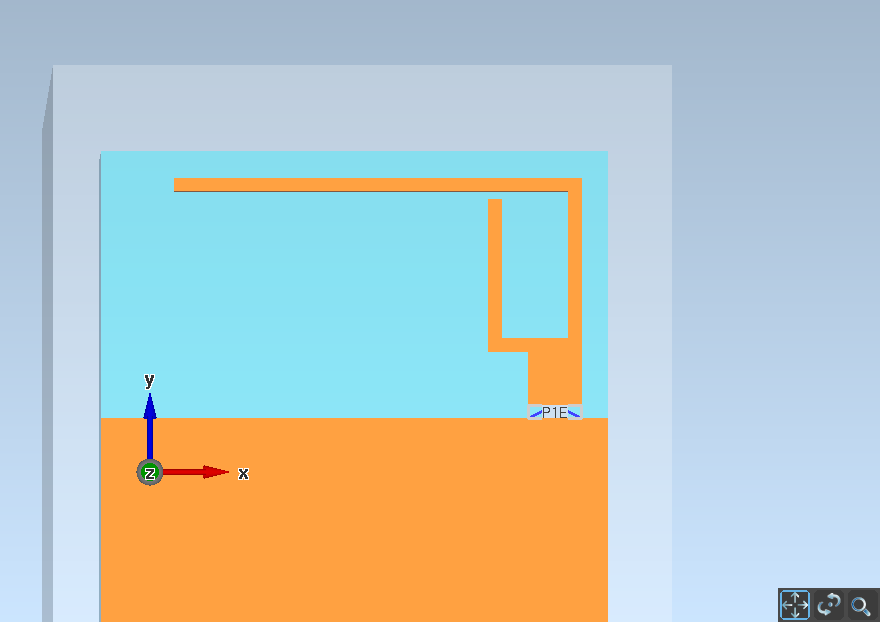
\includegraphics[width=0.7\textwidth]{../fig/plt/crazy_stuff_l4_pcb_v2c_laptop_1a_105_5ghz_3d_pcb_xy.png}
	\caption{2D Modell, Ansicht von oben}
\end{figure}


\subsection{Simulation}

\subsubsection{Aufbau}

\begin{figure}[h!]
	\centering
	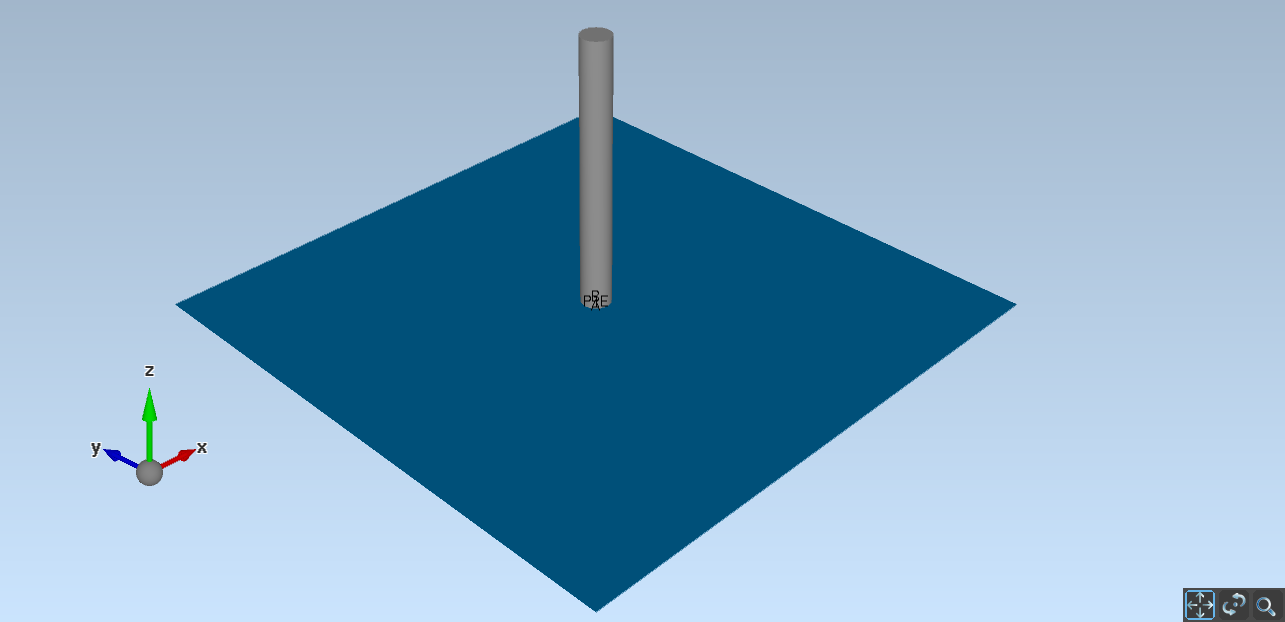
\includegraphics[width=0.75\textwidth]{../fig/plt/monopol_a_sim_3d_model.png}
	\caption{Erstelltes Simulationsmodell.}
\end{figure}

Das Simulationsmodell entspricht der zuvor vorgestellten Geometrie.
Für die Simulation wurde dem Modell noch eine Quelle hinzugefügt,
welche die Einspeisung repräsentiert. Diese ist zwischen dem
Stab und der Groundplane platziert, wodurch diese miteinander
über die Quelle verbunden werden.

\newpage
\subsubsection{Reflexionskoeffizient}

\begin{figure}[h!]
	\centering
	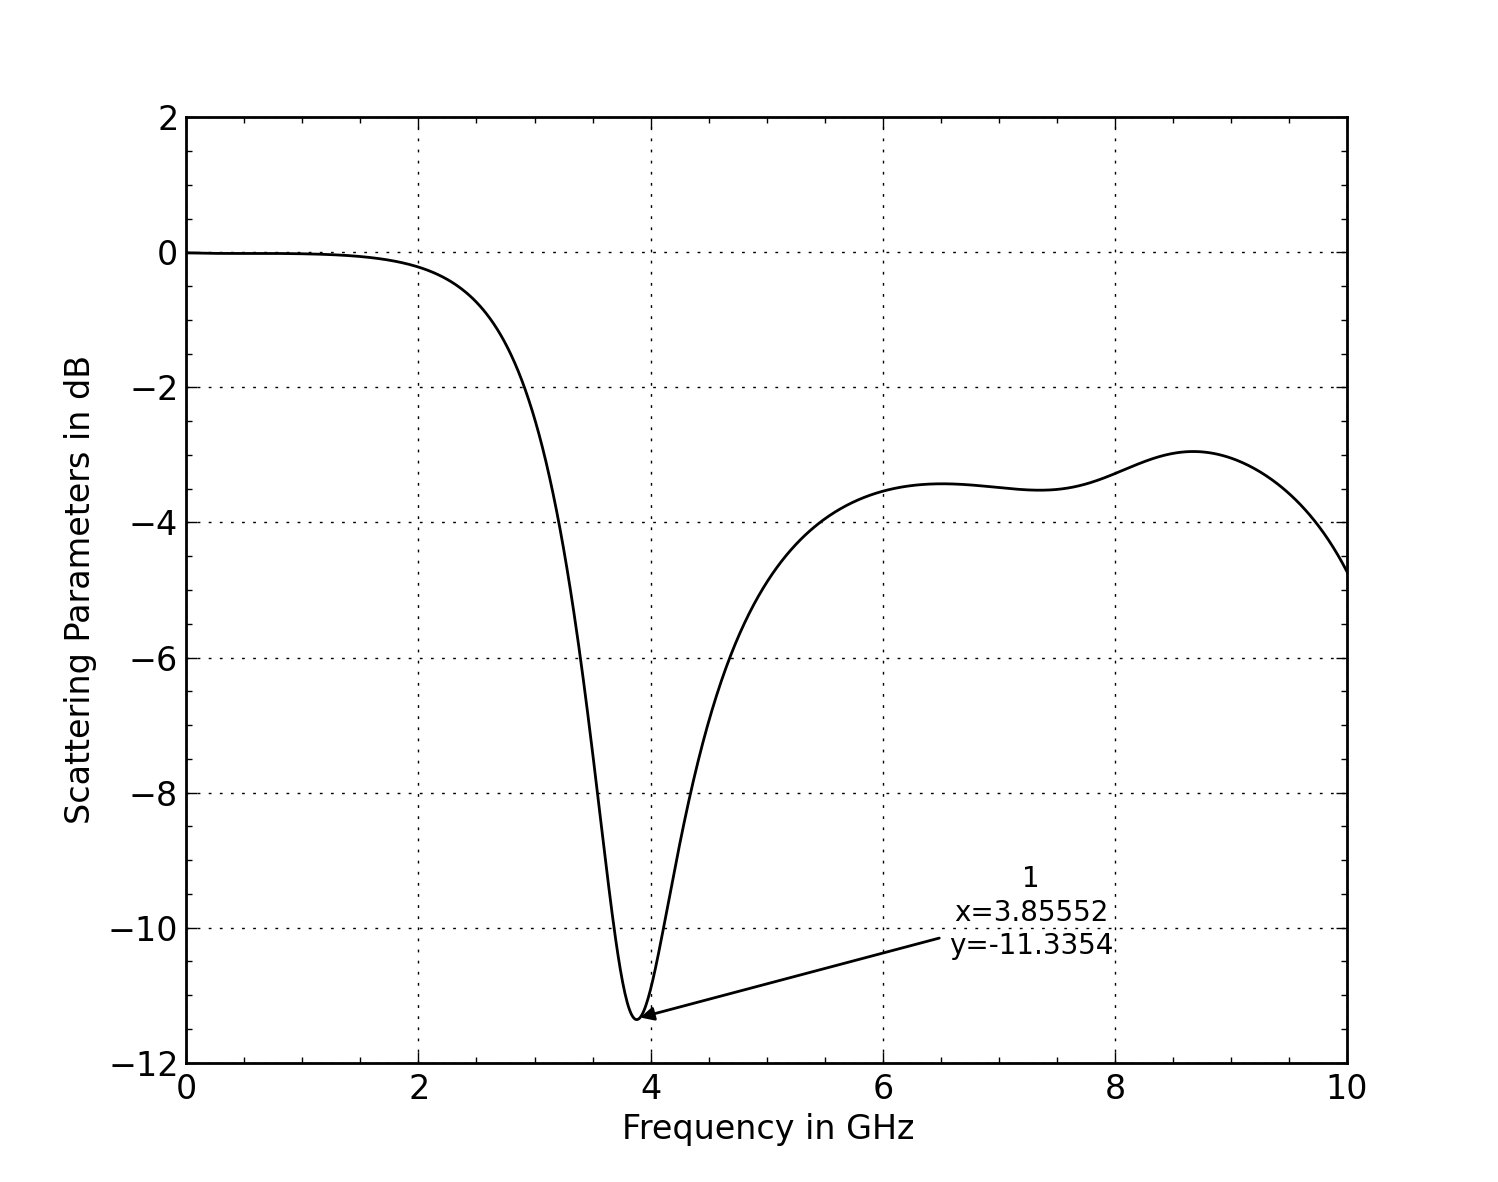
\includegraphics[width=0.75\textwidth]{../fig/plt/monopol_a_sim_s11.png}
	\caption{Reflexionskoeffizient ($S_{11}$ Parameter).}
\end{figure}

Die Simulation zeigt, dass die beste Abstrahlung leicht unter der
gewünschten Frequenz von \SI{4}{\giga\hertz} liegt. Dieses Ergebnis
kann nun in der Weise interpretiert werden, dass die erstellte
Antenne zu \emph{lang} ist. Durch die Kürzung der Stablänge $l_S$
kann dies korrigiert werden, denn damit wird die Wellenlänge
$\lambda$ reduziert und folglich die Frequenz erhöht.

\newpage
\subsubsection{Antennenimpedanz}

\begin{figure}[h!]
	\centering
	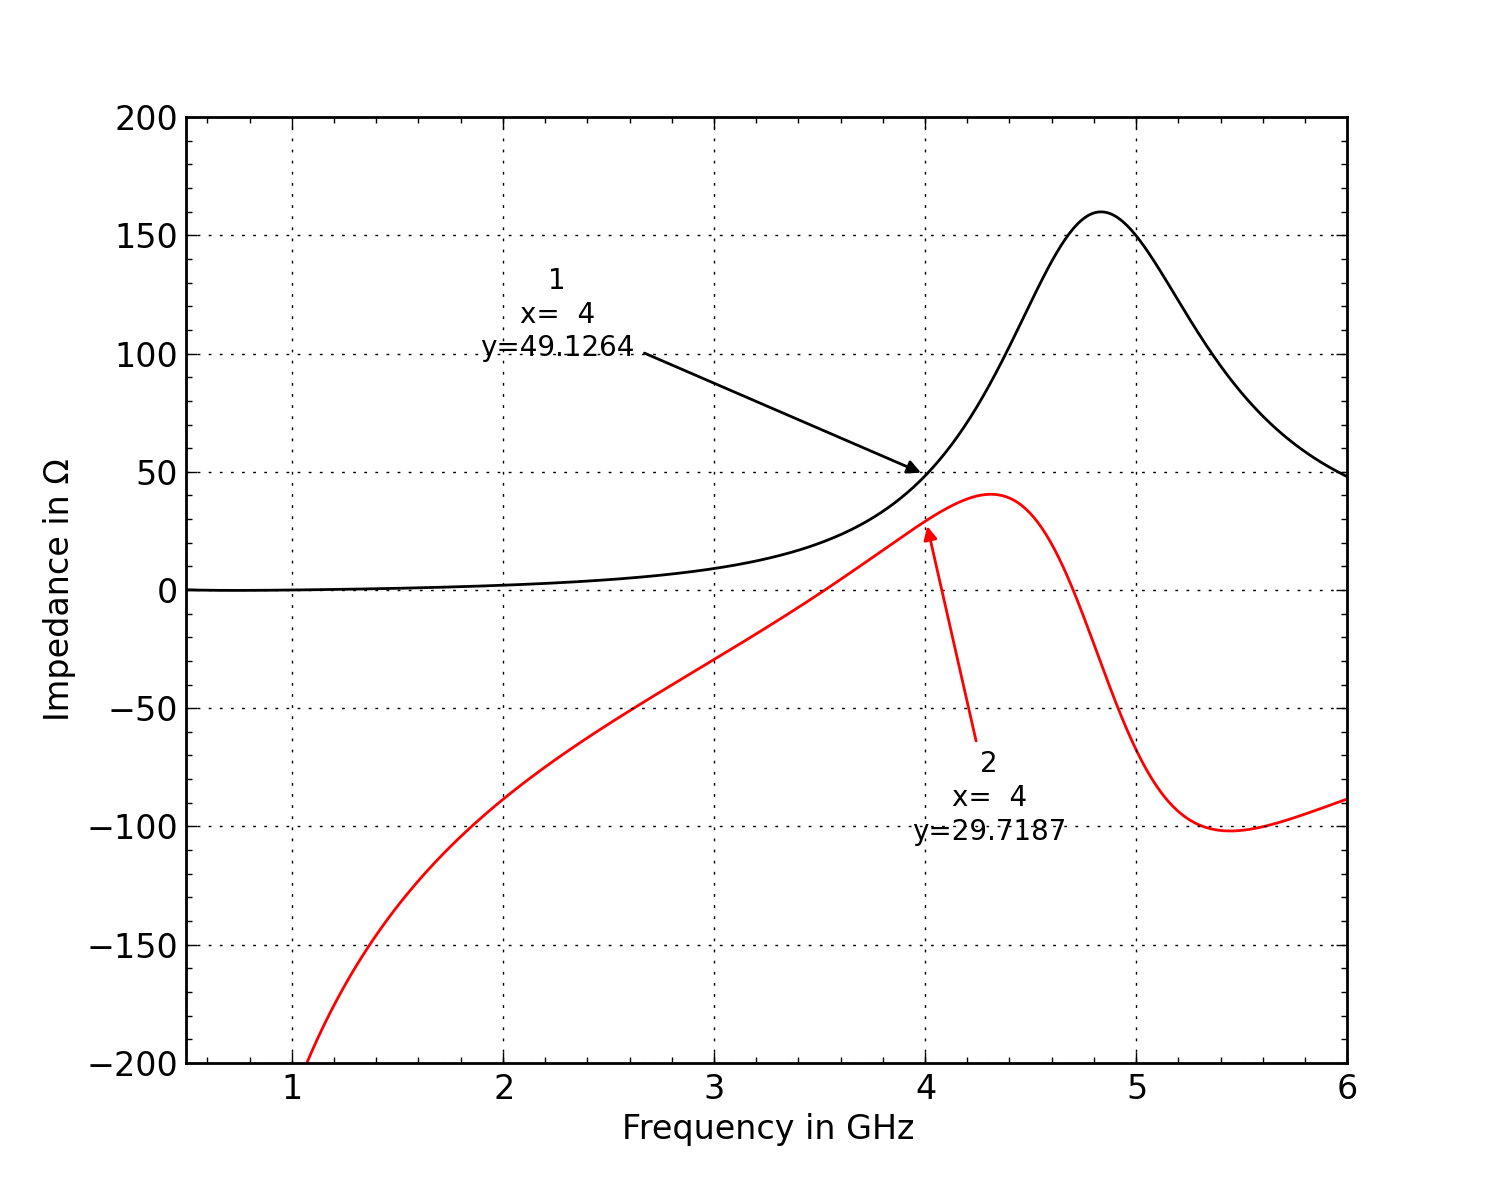
\includegraphics[width=0.75\textwidth]{../fig/plt/monopol_a_sim_impedance.png}
	\caption{Antennenimpedanz ($\mathrm{Re}\left\{Z\right\}$ schwarz,  $\mathrm{Im}\left\{Z\right\}$ rot).}
\end{figure}

Die Simulation zeigt, dass der Realanteil
$\mathrm{Re}\left\{Z\right\} \approx \SI{50}{\ohm}$ und somit dem
gewünschten Wert entspricht. Der Imaginäranteil ist mit
$\mathrm{Im}\left\{Z\right\} \approx \SI{30}{\ohm}$ deutlich über
dem geforderten Wert von \SI{0}{\ohm}, hat induktiven Charakter (da
$\mathrm{Im}\left\{Z\right\} > 0$) und bedeutet, dass eine suboptimale
Ausnutzung vorliegt (da ein Teil der Leistung nicht abstrahlungsfähig
ist durch die resultierende Reflexion). Weiter ist in der Abbildung ein
nahe liegener Resonanzpunkt zu erkennen bei ca. \SI{4.8}{\giga\hertz}.
Da dieser Resonanzpunkt nahe liegt und die Impedanz in dessen Umgebung
eine hohe Änderungsrate $\frac{\mathrm{d}Z}{\mathrm{d}f}$ besitzt,
bedeutet dies, dass die Impedanzverhältnisse nicht robust und die
Antenne \emph{empfindlich} ist auf eine Änderung der Frequenz $f$.
Die Simulation zeigt, dass eine Änderung der Frequenz um 
\SI{400}{\mega\hertz} den Realanteil der Impedanz bereits
verdoppelt auf \SI{100}{\ohm}.


\newpage
\subsubsection{2D Richtdiagramm}

\begin{figure}[h!]
	\centering
	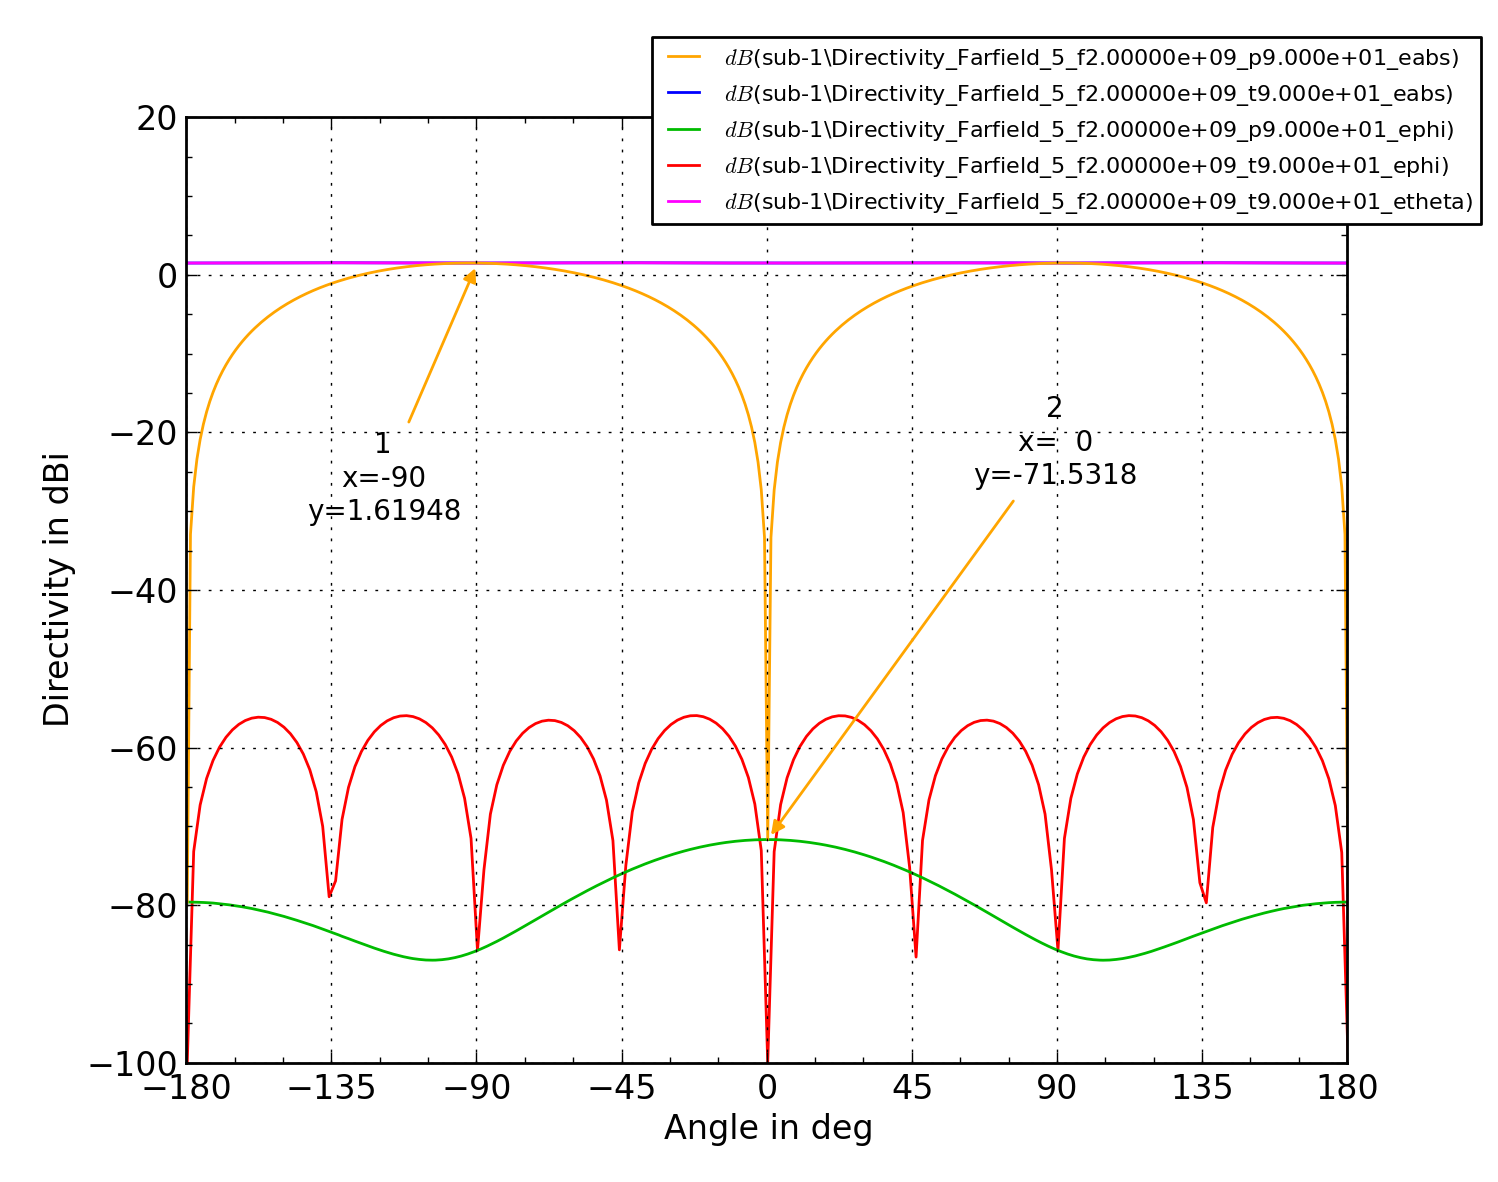
\includegraphics[width=0.75\textwidth]{../fig/plt/monopol_a_sim_2d_pattern.png}
	\caption{2D Richtdiagramm.}
\end{figure}

Die Simulation zeigt, dass die Antenne die erwatrete Abstrahlcharakteristik
eines idealen Monopols aufweist, welcher eine maximale Abstrahlung bei
$\pm \SI{90}{\degree}$ (senkrecht zum Stab) und die minimale Abstrahlung
bei \SI{0}{\degree} respektive \SI{180}{\degree} (entland des Stabs)
aufweist ($E_{\mathrm{abs}}$).

\newpage
\subsubsection{3D Richtdiagramm}

\begin{figure}[h!]
	\centering
	%\begin{subfigure}[b]{0.48\textwidth}
		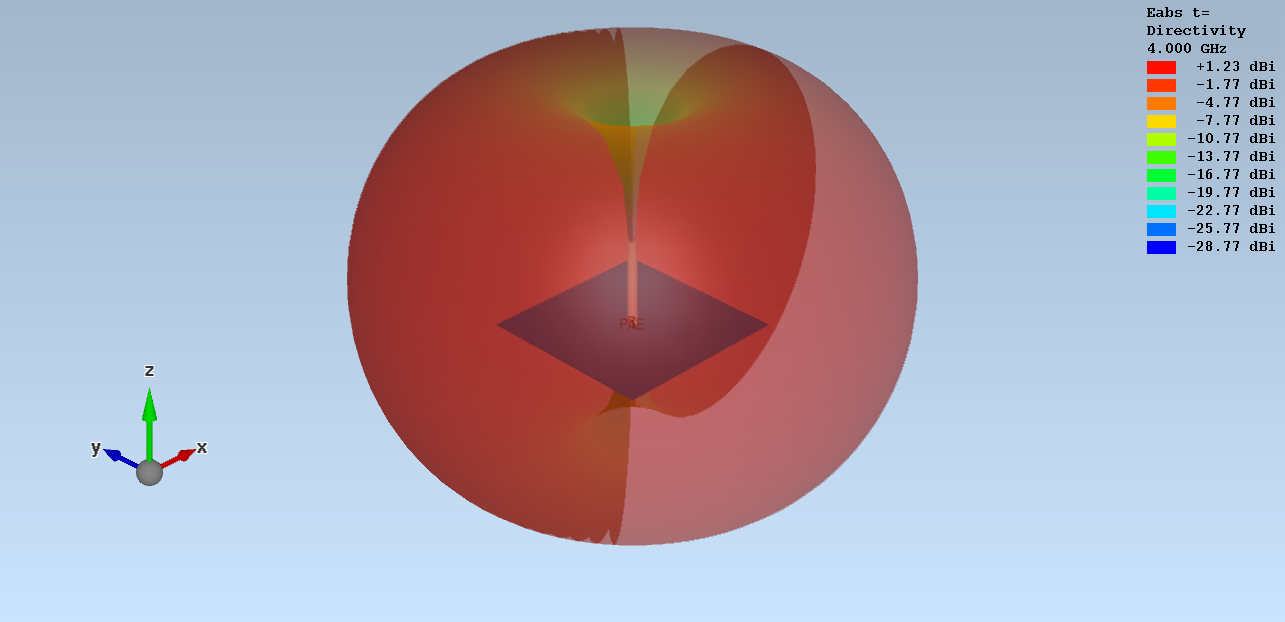
\includegraphics[width=1\textwidth]{../fig/plt/monopol_a_sim_3d_eabs.png}
	%	\caption{E-Feld Absolut}
	%\end{subfigure}
	%\begin{subfigure}[b]{0.48\textwidth}
	%	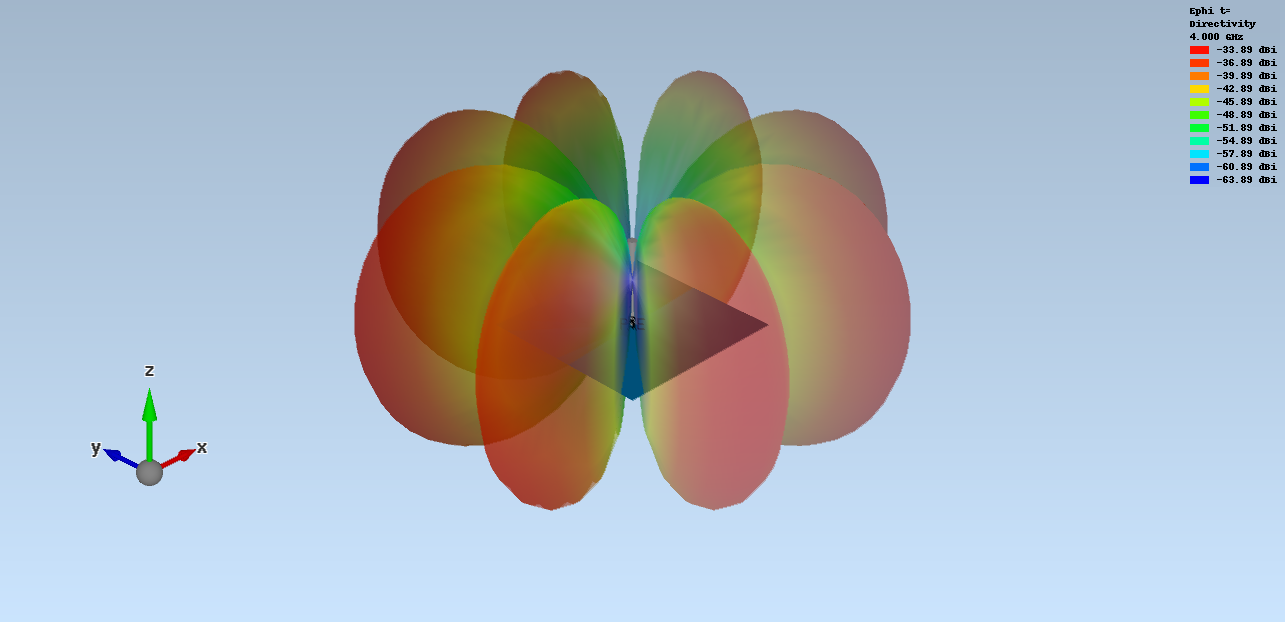
\includegraphics[width=1\textwidth]{../fig/plt/monopol_a_sim_3d_ephi.png}
	%	\caption{E-Feld $\varphi$}
	%\end{subfigure}
	\caption{3D Darstellung des Fernfeldes}
\end{figure}

Die Simulation zeigt wie bereits das 2D Richtdiagramm die Abstrahlung
der Antenne ($E_{\mathrm{abs}}$). Hier ist nochmals deutlich zu sehen,
dass die Antenne \emph{seitwärts} gut abstrahlt, \emph{auf-} und
\emph{abwärts} jedoch ein \emph{Funkloch} besteht.
	\clearpage
\section{Messungen}
Die entwickelte Platine

\begin{figure}[h!]
	\centering
	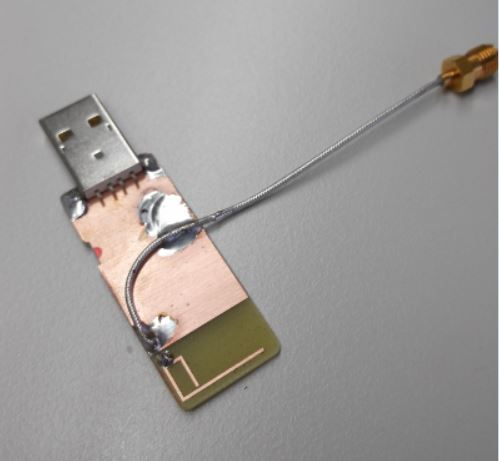
\includegraphics[width=0.5\textwidth, angle = 180]{../fig/plt/Platine.JPG}
	\caption{Die entwickelte Platine}
	\label{fig:Platine}
\end{figure}


\subsection{Messungen mit dem Netzwerkanalyzer}

Marke: Rhode$\&$Schwartz\\
Inventarnr.: 14006

\vspace*{3mm}

Vor dem Einsatz des Netzwerkanalyzers wurde dieser kalibiert.

\begin{figure}[h!]
	\centering
	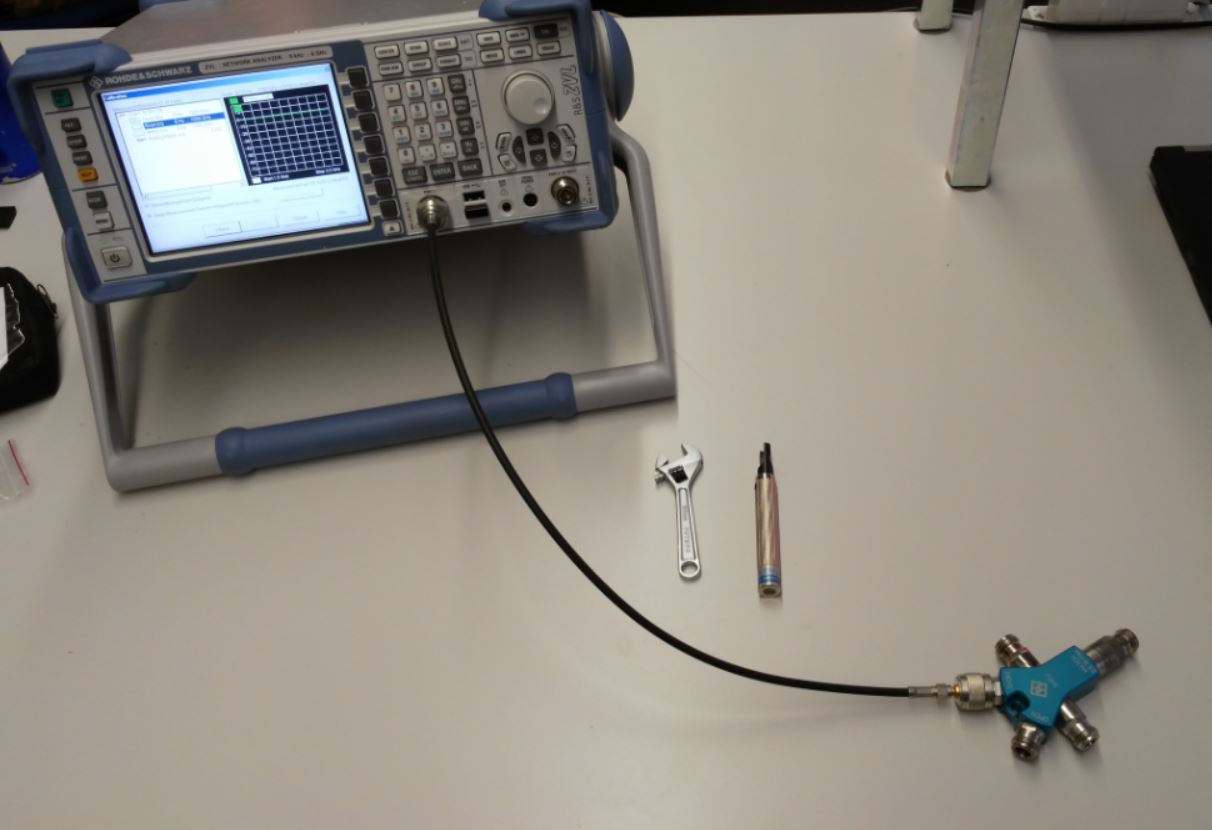
\includegraphics[width=0.8\textwidth]{../fig/plt/Calib.JPG}
	\caption{Kalibrierung des Netzwerkanalyzers}
	\label{fig:calib}
\end{figure}

Mit dem Netzwerkanalyzer wurden Messungen ohne und mit Gehäuse gemacht
bei \SI{2.4}{\giga\hertz} und \SI{5}{\giga\hertz}. In diesem Bericht
wird der Fokus auf die Messung mit Gehäuse gelegt. Zum einen Überblick
über das gesamte Frequenzspektrum zu vermitteln. Abbildungen x zeigen
einen Überblick über das gesamte Frequenzspektrum von
\SI{1.75}{\giga\hertz} bis \SI{5.75}{\giga\hertz}. Im Abschnitt x und
Abschnitt y wird auf die Messungen bei den spezifischen Designfrequenzen
eingegangen.

\begin{figure}[h!]
	\begin{center}
		\begin{subfigure}[t]{0.49\textwidth}
			\begin{center}
				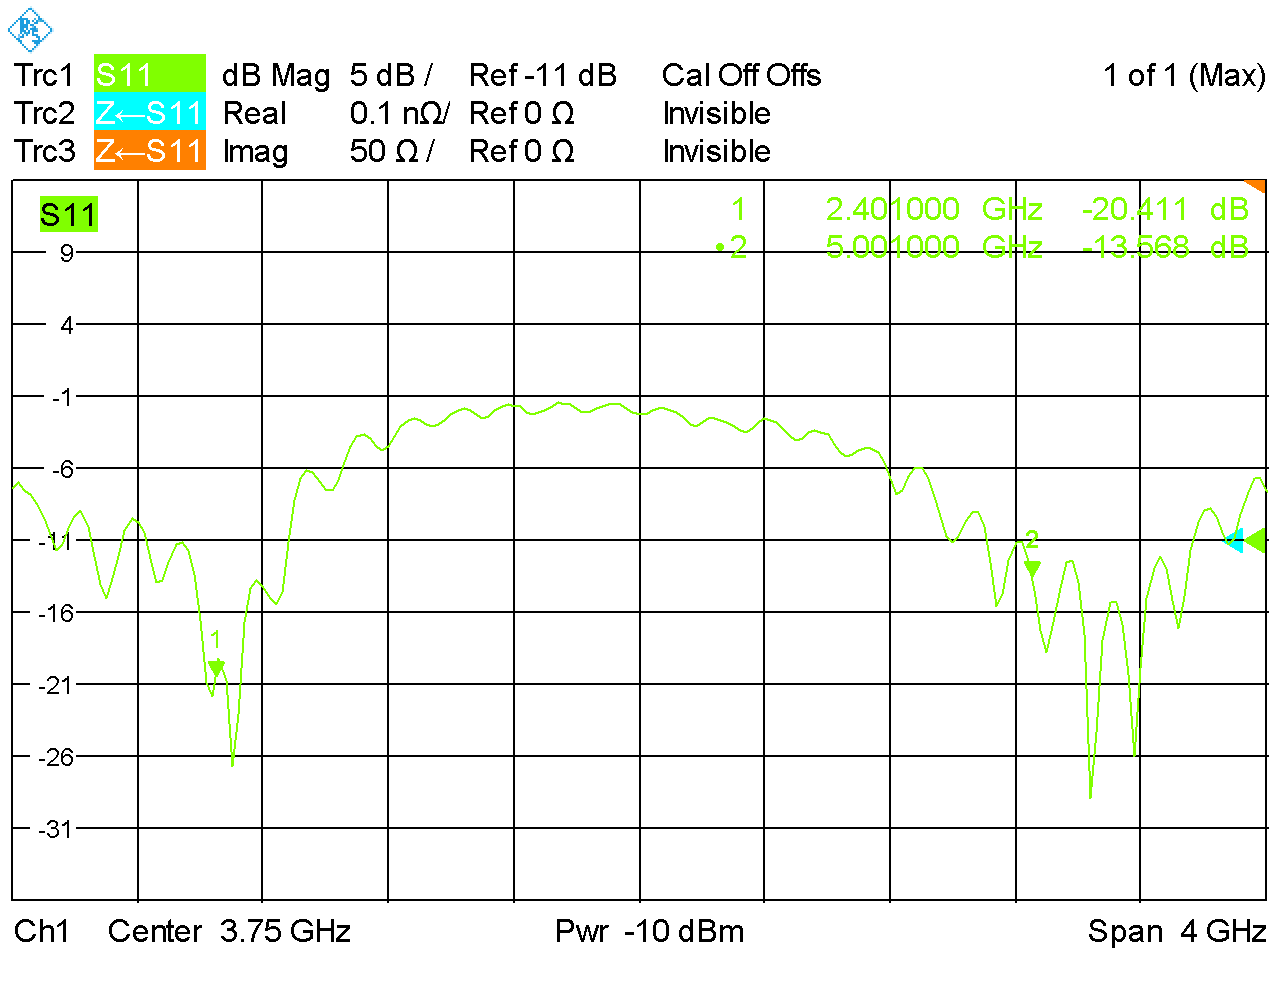
\includegraphics[width=1\textwidth]{../fig/plt/S11_WITH_FULL.PNG}
				\caption{Reflexionskoeffizient}
				\label{fig:S11_with_full}
			\end{center}
		\end{subfigure}
		\begin{subfigure}[t]{0.49\textwidth}
			\begin{center}
				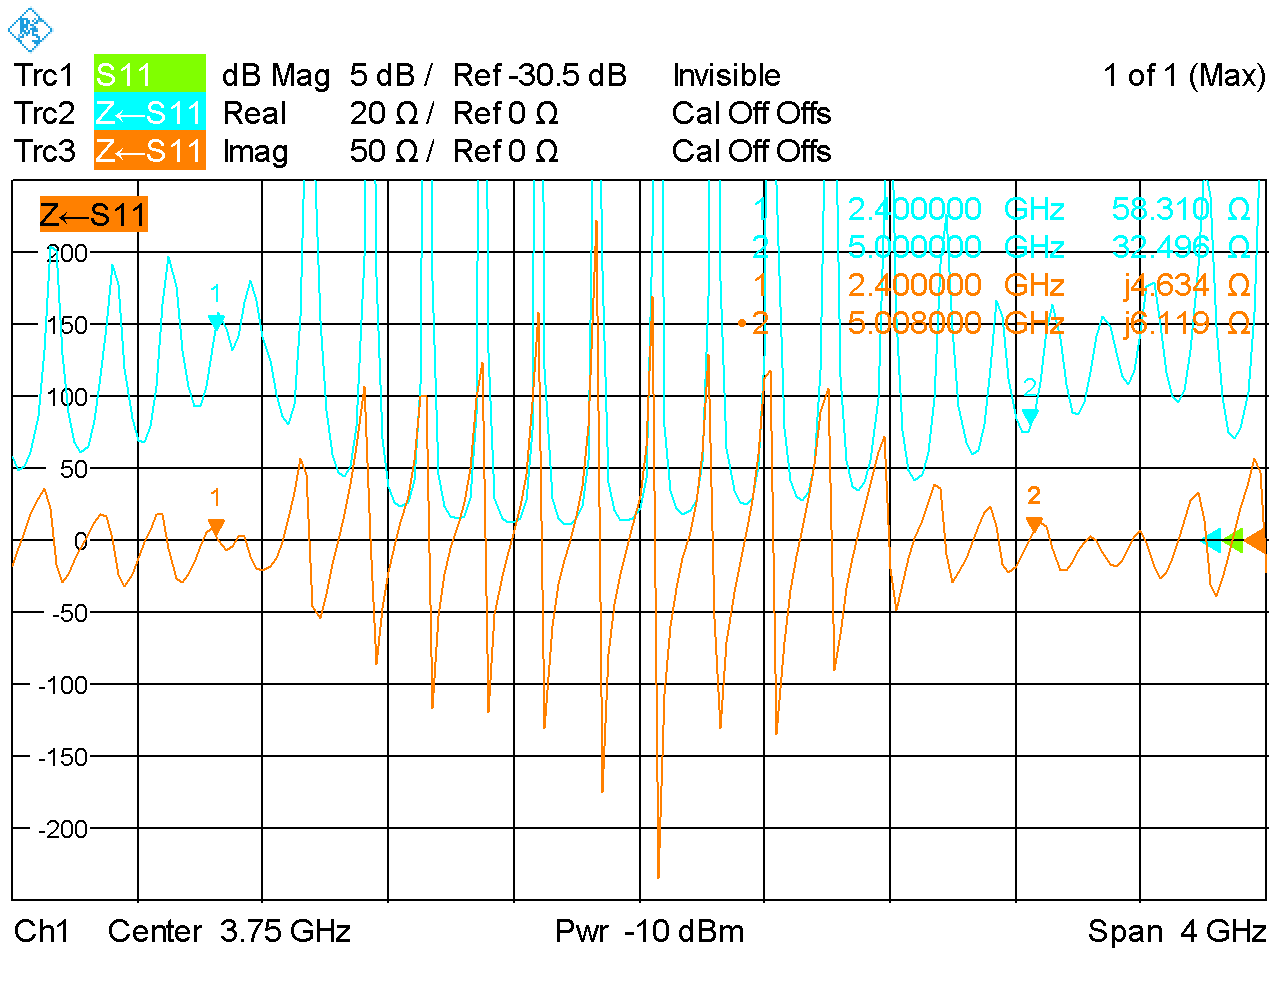
\includegraphics[width=1\textwidth]{../fig/plt/IMP_WITH_FULL.PNG}
				\caption{Impedanz}
				\label{fig:Imp_with_full}
			\end{center}
		\end{subfigure}
		\caption{Überblick über gesamtes Frequenzspektrum}
		\label{fig:full}
	\end{center}
\end{figure}


\clearpage
\subsubsection{Reflexionskoeffizient S11}

Bei 2.4 GHz zeigte sich ein äusserst ausgeprägter Reflexionskoeffizent kleiner als -50dB

\begin{figure}[h!]
	\begin{center}
		\begin{subfigure}[t]{0.49\textwidth}
			\begin{center}
				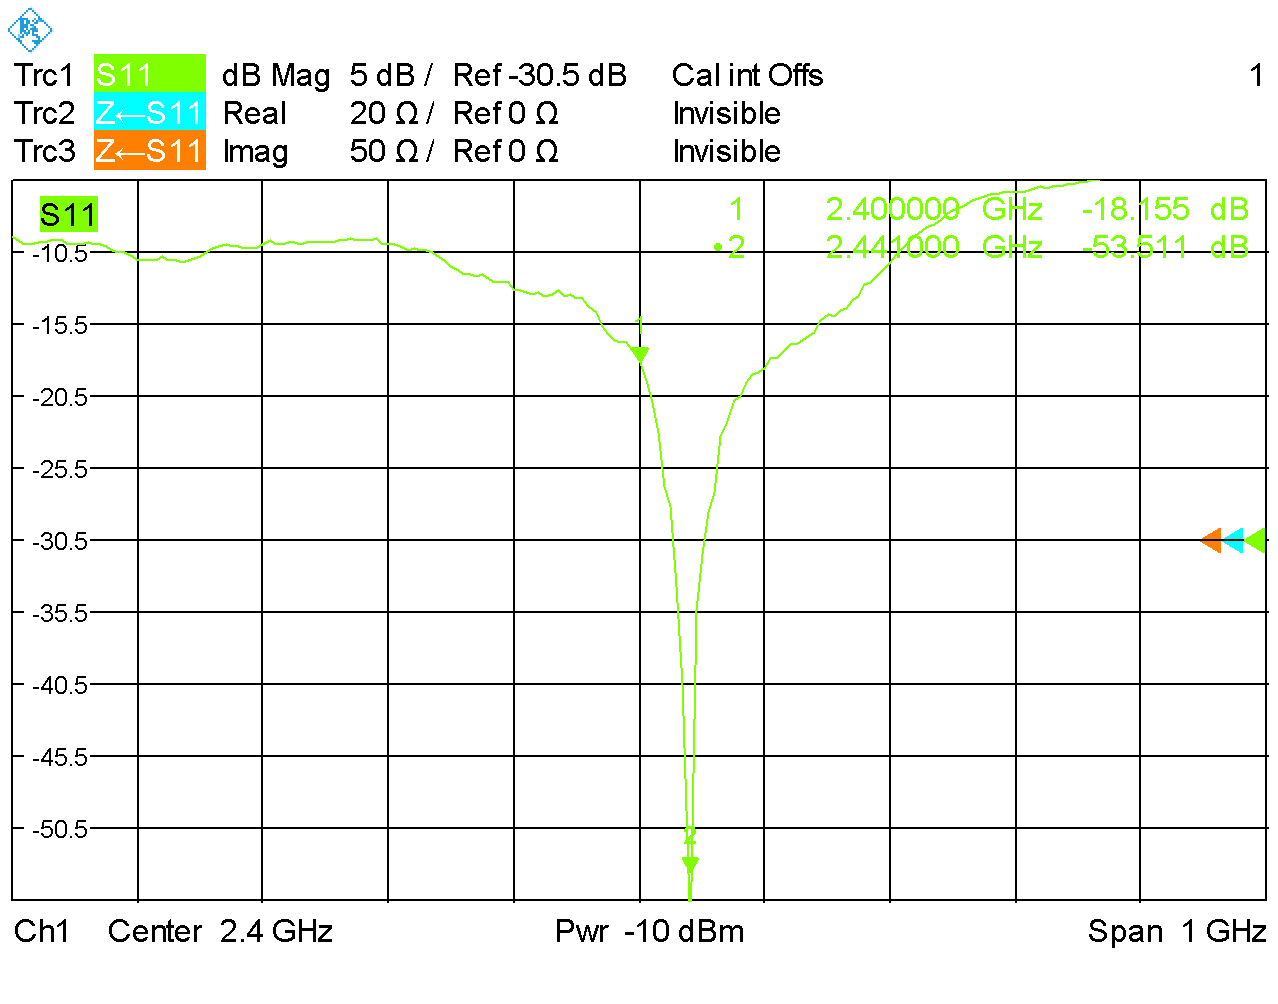
\includegraphics[width=1\textwidth]{../fig/plt/S11_WITH_2_4.PNG}
				\caption{bei 2.4 GHz}
				\label{fig:S11_with_full_2.4}
			\end{center}
		\end{subfigure}
		\begin{subfigure}[t]{0.49\textwidth}
			\begin{center}
				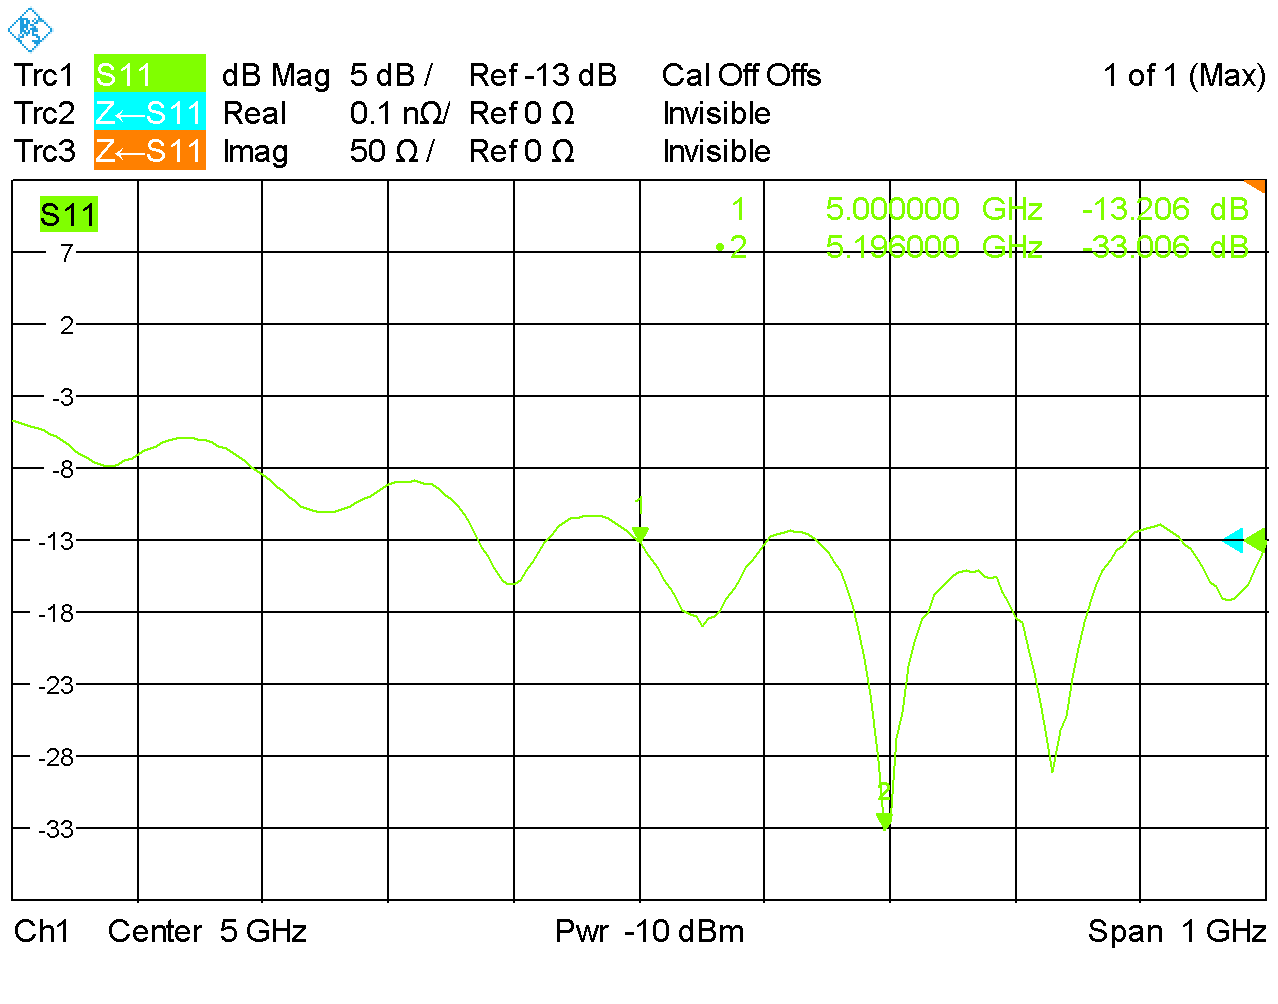
\includegraphics[width=1\textwidth]{../fig/plt/S11_WITH_5_0.PNG}
				\caption{bei 5.0 GHz}
				\label{fig:S11_with_full_5.0}
			\end{center}
		\end{subfigure}
		\caption{Reflexionskoeffizient S11}
		\label{fig:S11_each}
	\end{center}
\end{figure}

\subsubsection{Impedanz}

\begin{figure}[h!]
	\begin{center}
		\begin{subfigure}[t]{0.49\textwidth}
			\begin{center}
				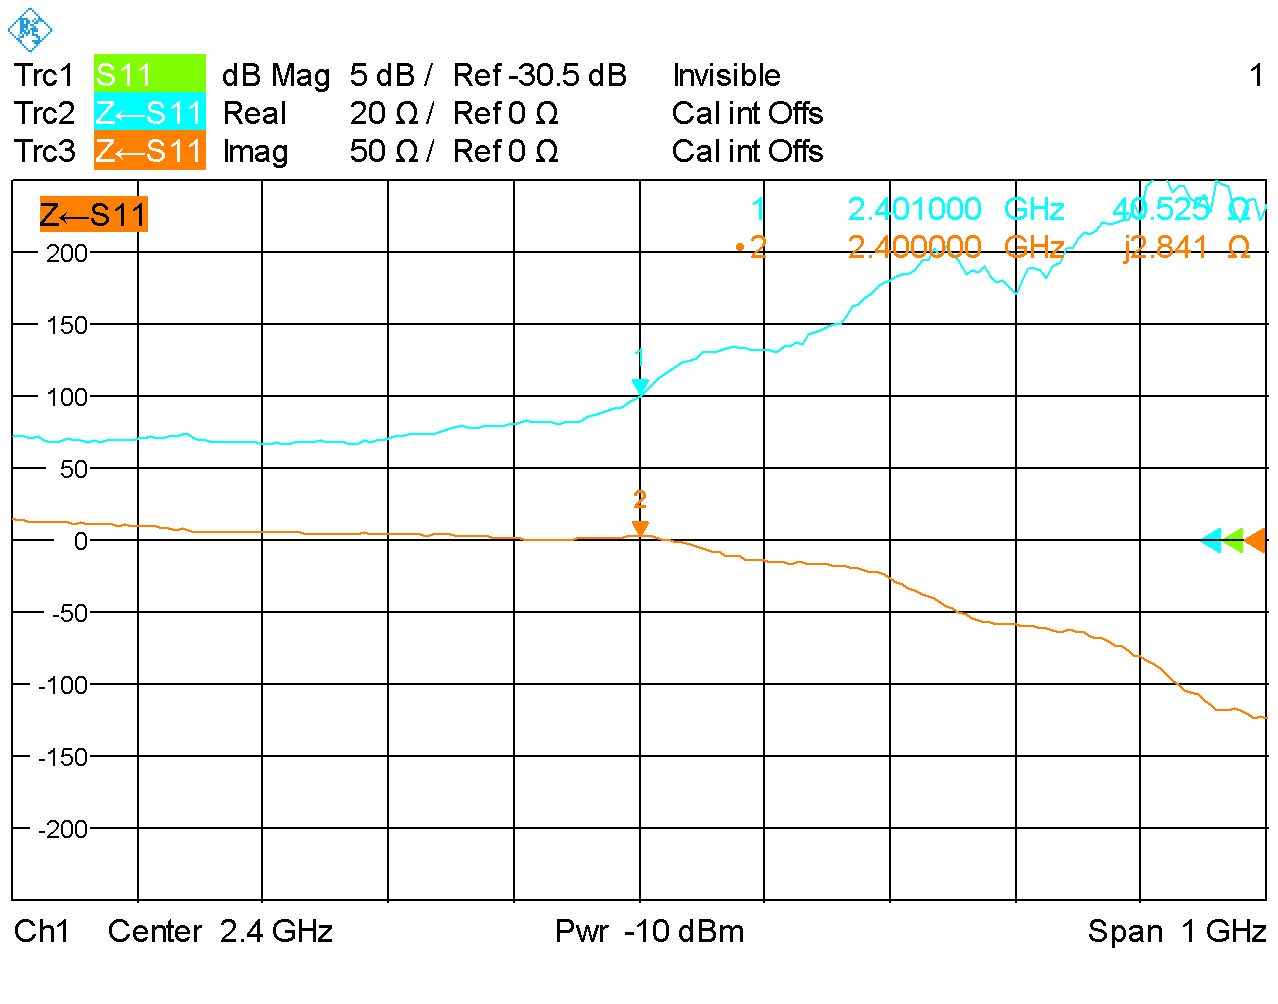
\includegraphics[width=1\textwidth]{../fig/plt/IMP_WITH_2_4.PNG}
				\caption{bei 2.4 GHz, !Achtung falsche Skala!}
				\label{fig:Imp_with_full_2.4}
			\end{center}
		\end{subfigure}
		\begin{subfigure}[t]{0.49\textwidth}
			\begin{center}
				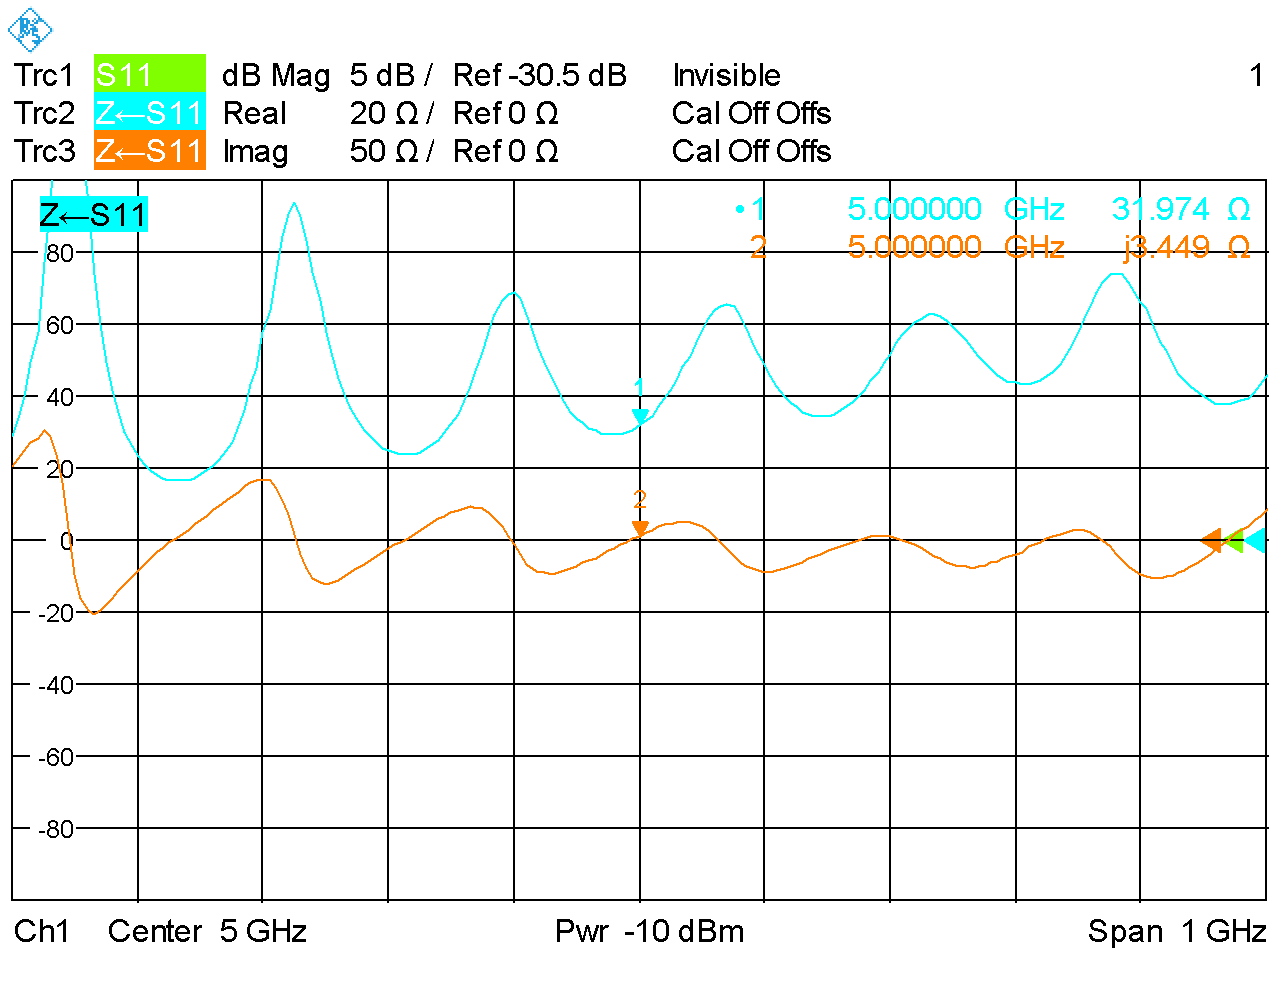
\includegraphics[width=1\textwidth]{../fig/plt/IMP_WITH_5_0.PNG}
				\caption{bei 5.0 GHz}
				\label{fig:Imp_with_full_5.0}
			\end{center}
		\end{subfigure}
		\caption{Impedanzen}
		\label{fig:Imp_each}
	\end{center}
\end{figure}

\newpage
\subsection{Messungen mit dem Starlab}
\begin{figure}[h!]
	\centering
	\def\svgscale{0.75}
	\input{../fig/gph/starlab_setup_annotated.pdf_tex}
	\caption{Aufbau der Messung im StarLab.}
	\label{fig:LaptopimStarlab}
\end{figure}

%\begin{figure}[h!]
%	\centering
%	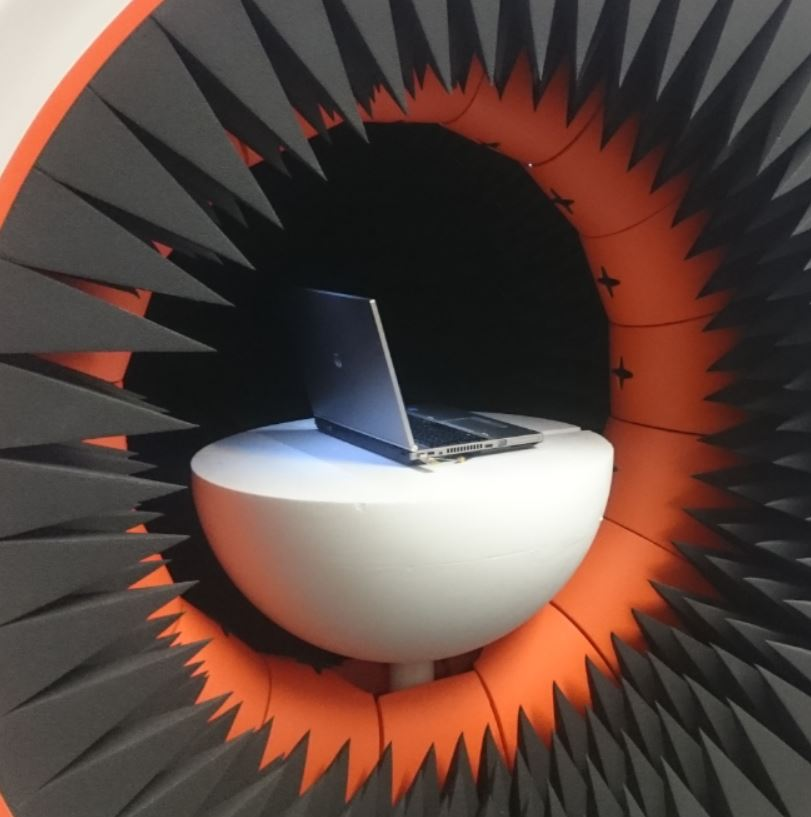
\includegraphics[width=0.6\textwidth]{../fig/plt/LaptopimStarLab.JPG}
%	\caption{DUT eingesteckt am Laptop im LinearScanner}
%	\label{fig:LaptopimStarlab}
%\end{figure}

\clearpage
\subsubsection{Abstrahlung 3D}

\begin{figure}[h!]
	\centering
	\begin{subfigure}[t]{0.35\textwidth}
		\begin{center}
			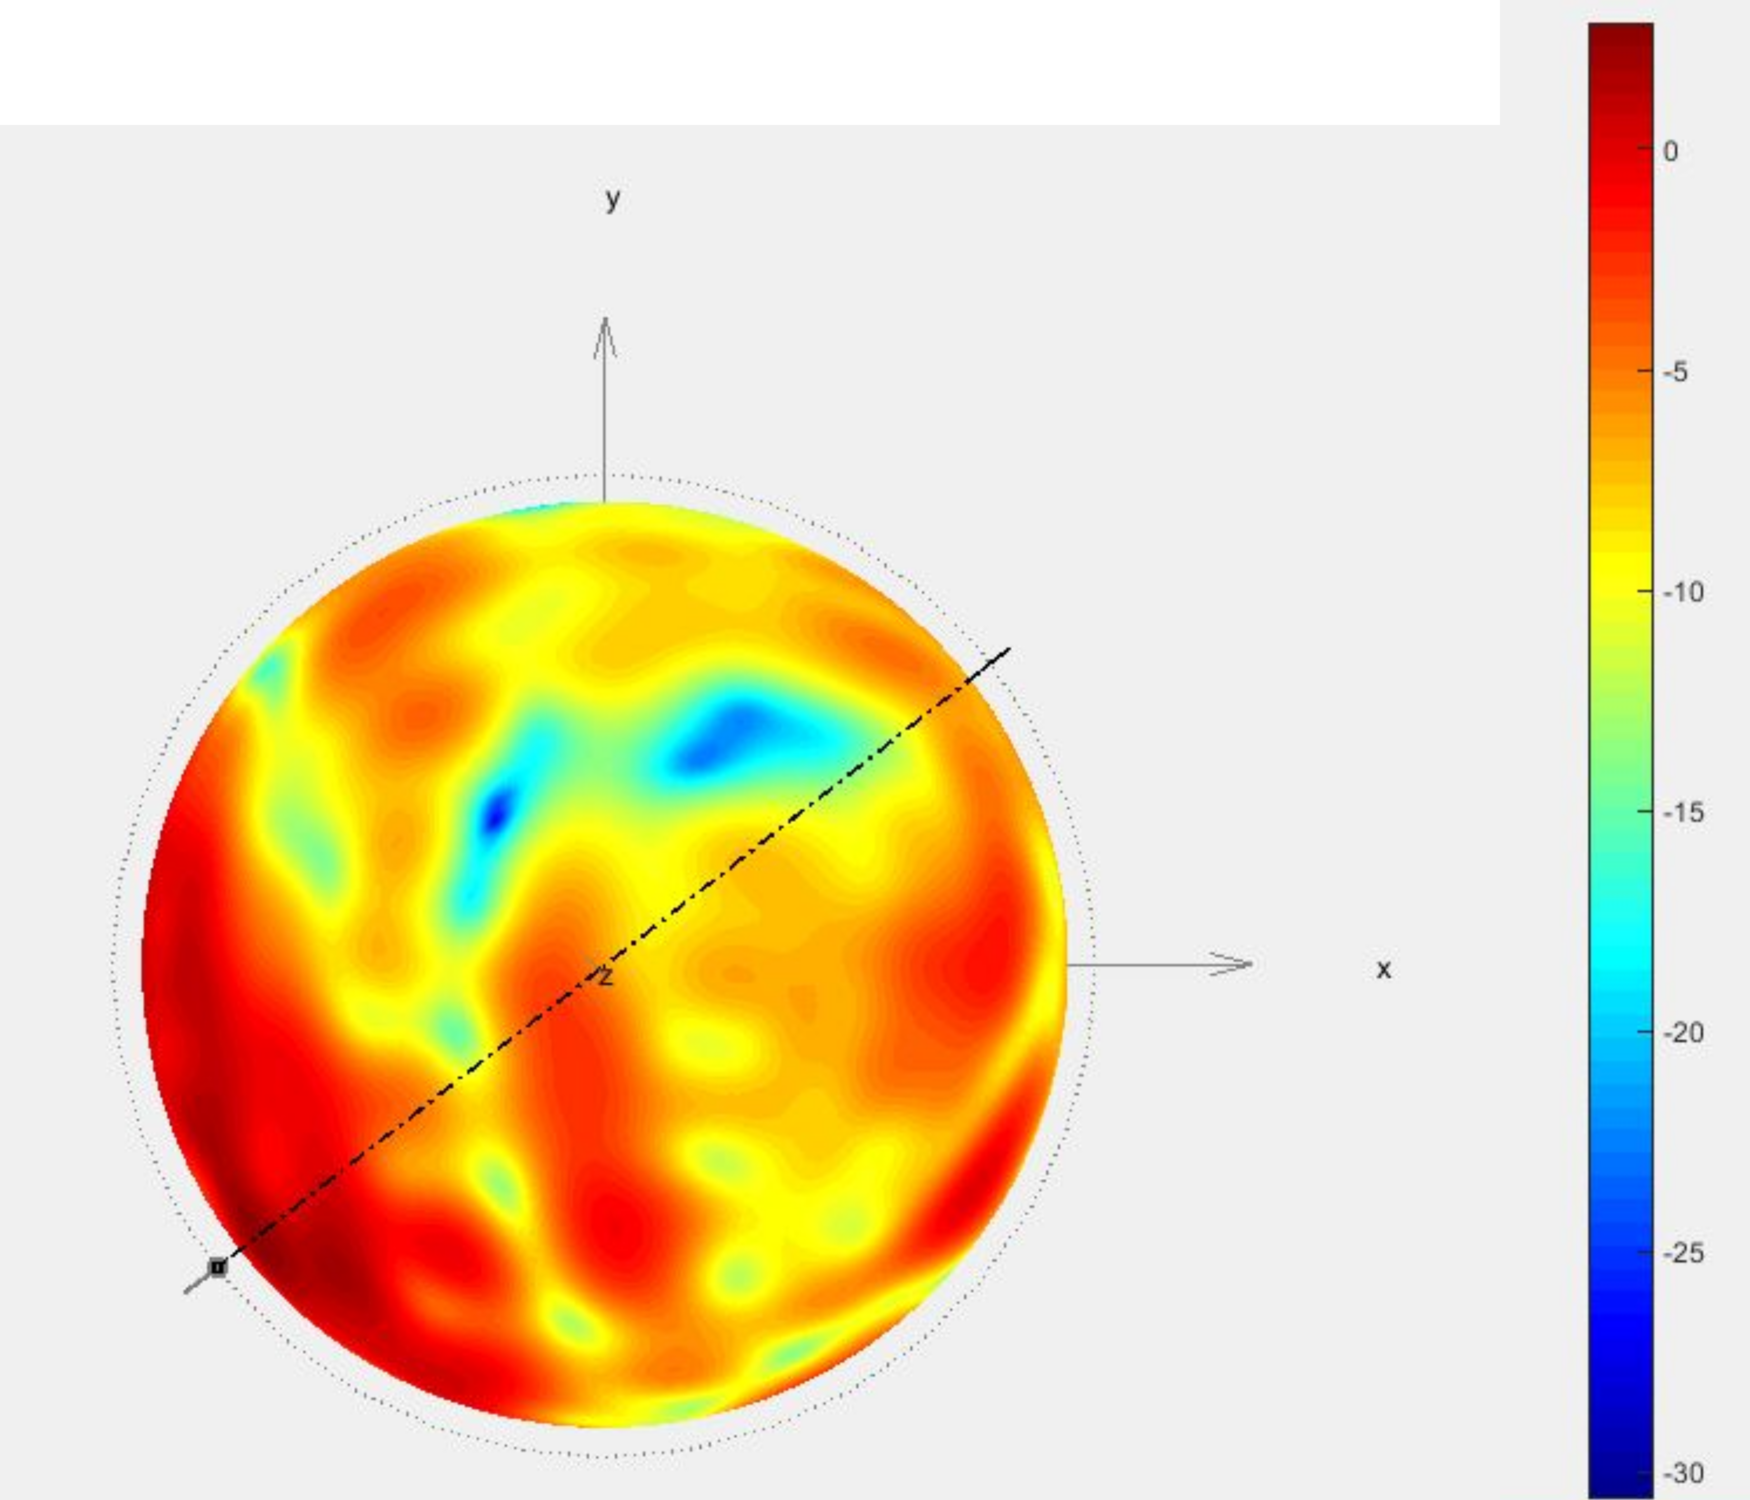
\includegraphics[width=1\textwidth]{../fig/plt/star_lab_2ghz4_xy_reduced.png}
			\caption{$\vec{E_{tot}}$ XY \SI{2.4}{\giga\hertz}}
		\end{center}
	\end{subfigure}
	\begin{subfigure}[t]{0.35\textwidth}
		\begin{center}
			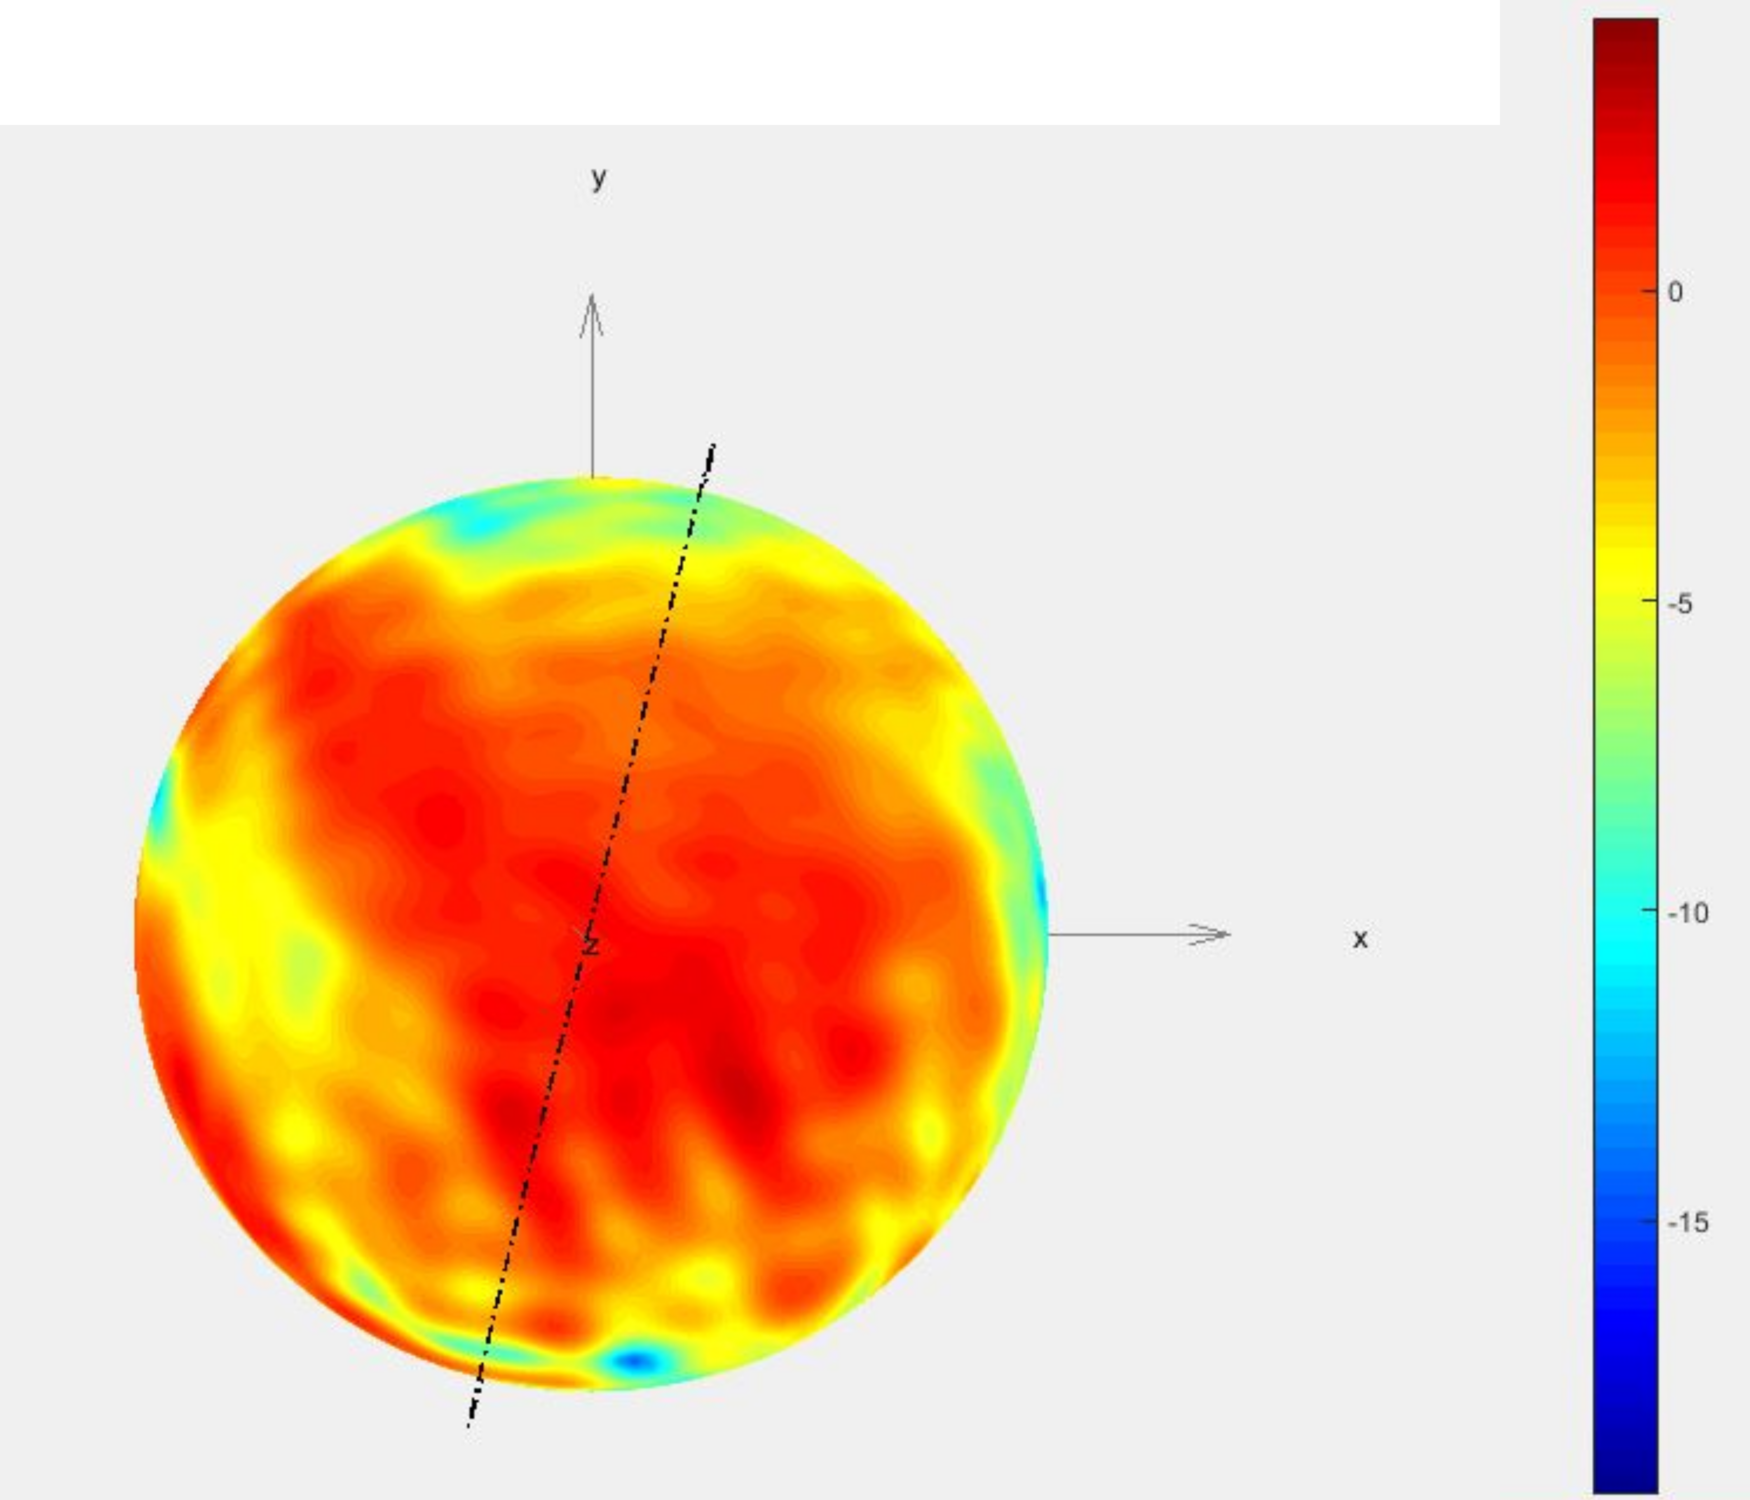
\includegraphics[width=1\textwidth]{../fig/plt/star_lab_5ghz0_xy_reduced.png}
			\caption{$\vec{E_{tot}}$XY \SI{5.0}{\giga\hertz}}
		\end{center}
	\end{subfigure}
	
	\begin{subfigure}[t]{0.35\textwidth}
		\begin{center}
			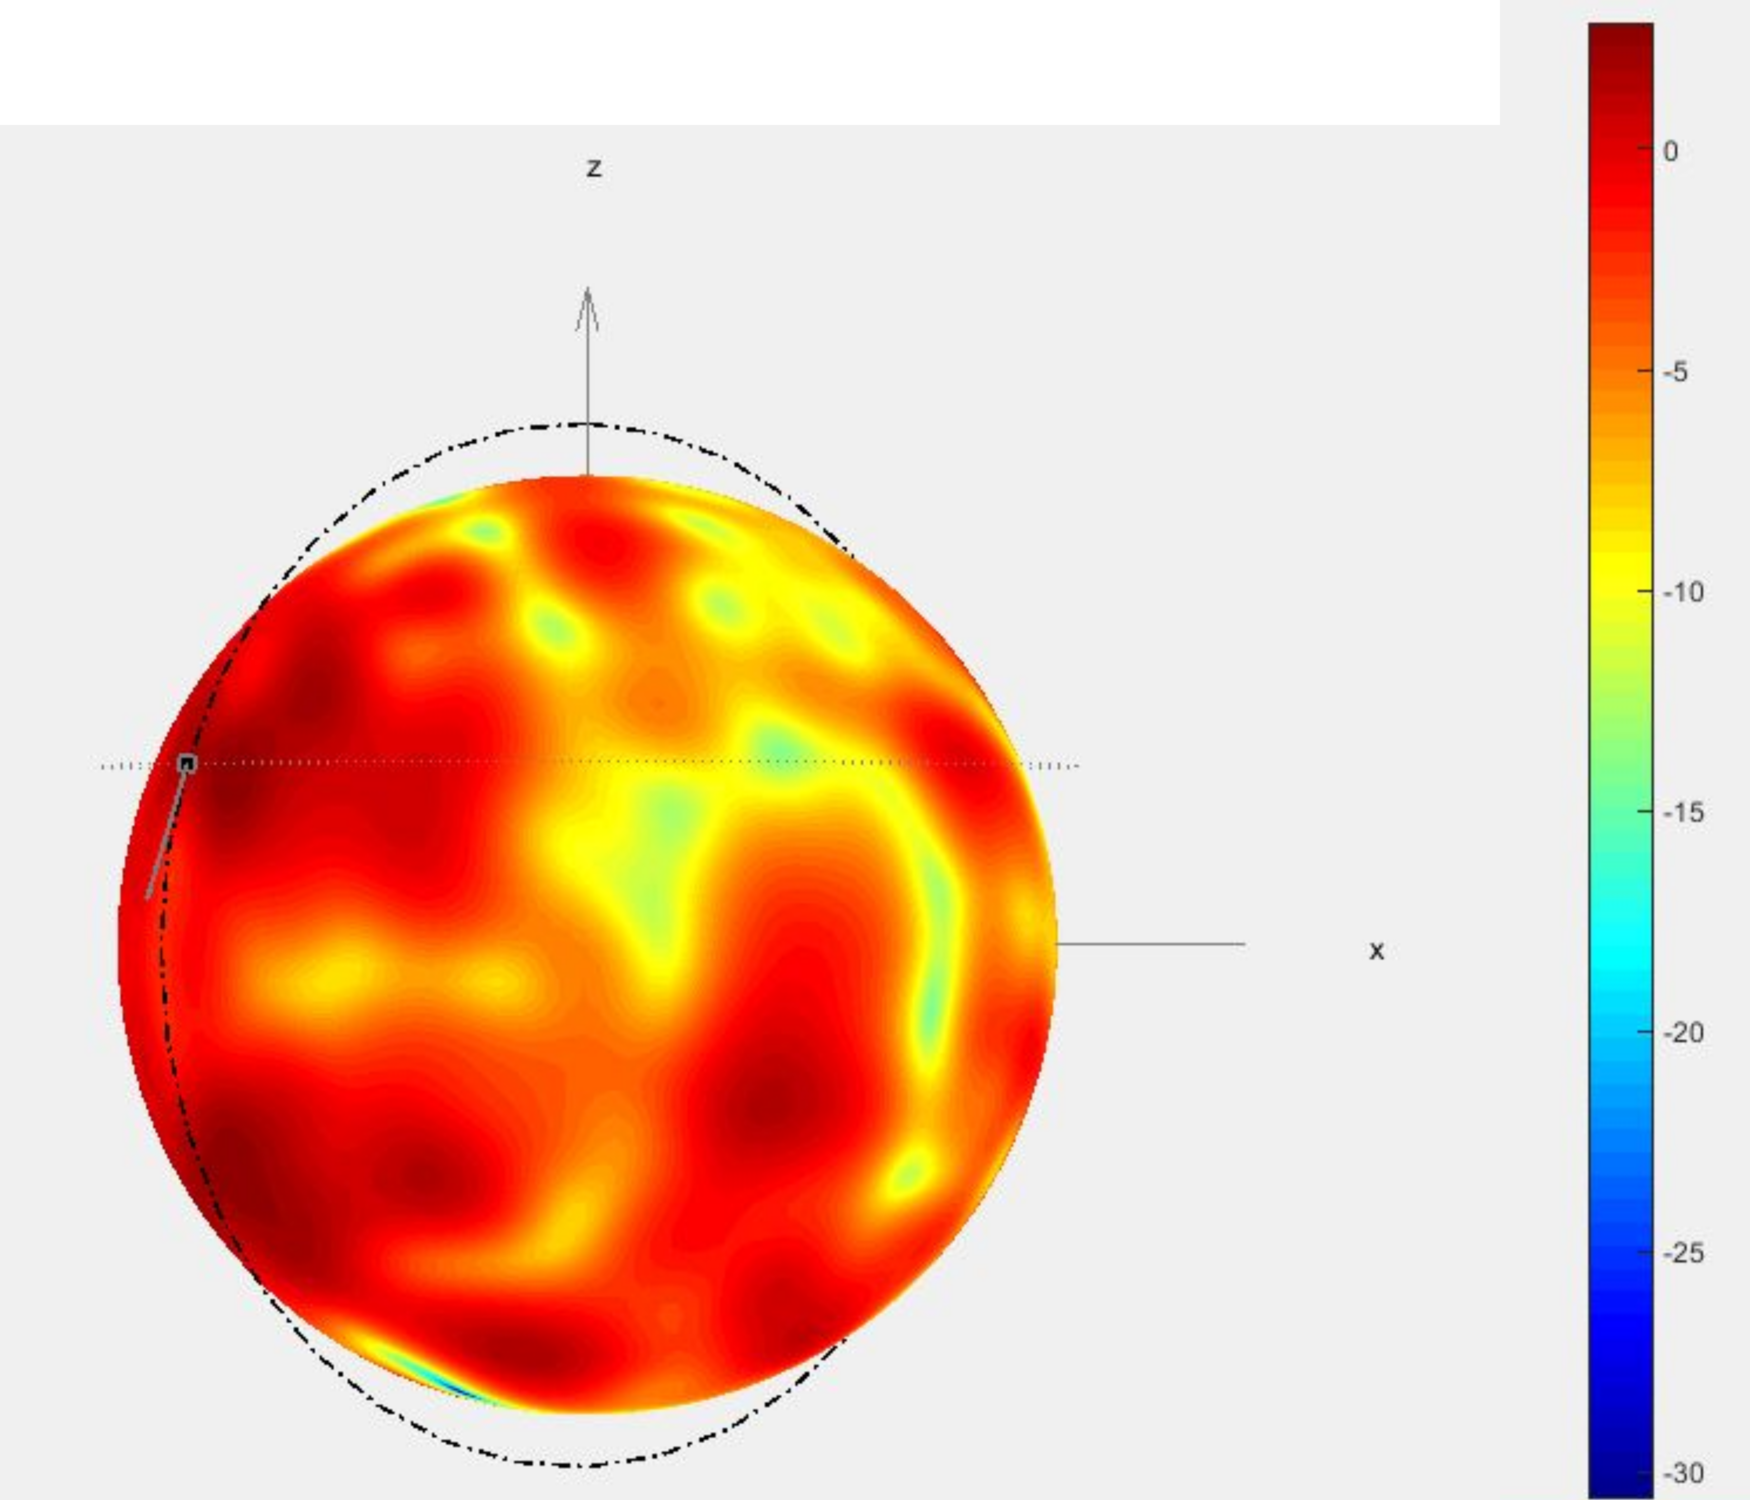
\includegraphics[width=1\textwidth]{../fig/plt/star_lab_2ghz4_xz_reduced.png}
			\caption{$\vec{E_{tot}}$XZ \SI{2.4}{\giga\hertz}}
		\end{center}
	\end{subfigure}
	\begin{subfigure}[t]{0.35\textwidth}
		\begin{center}
			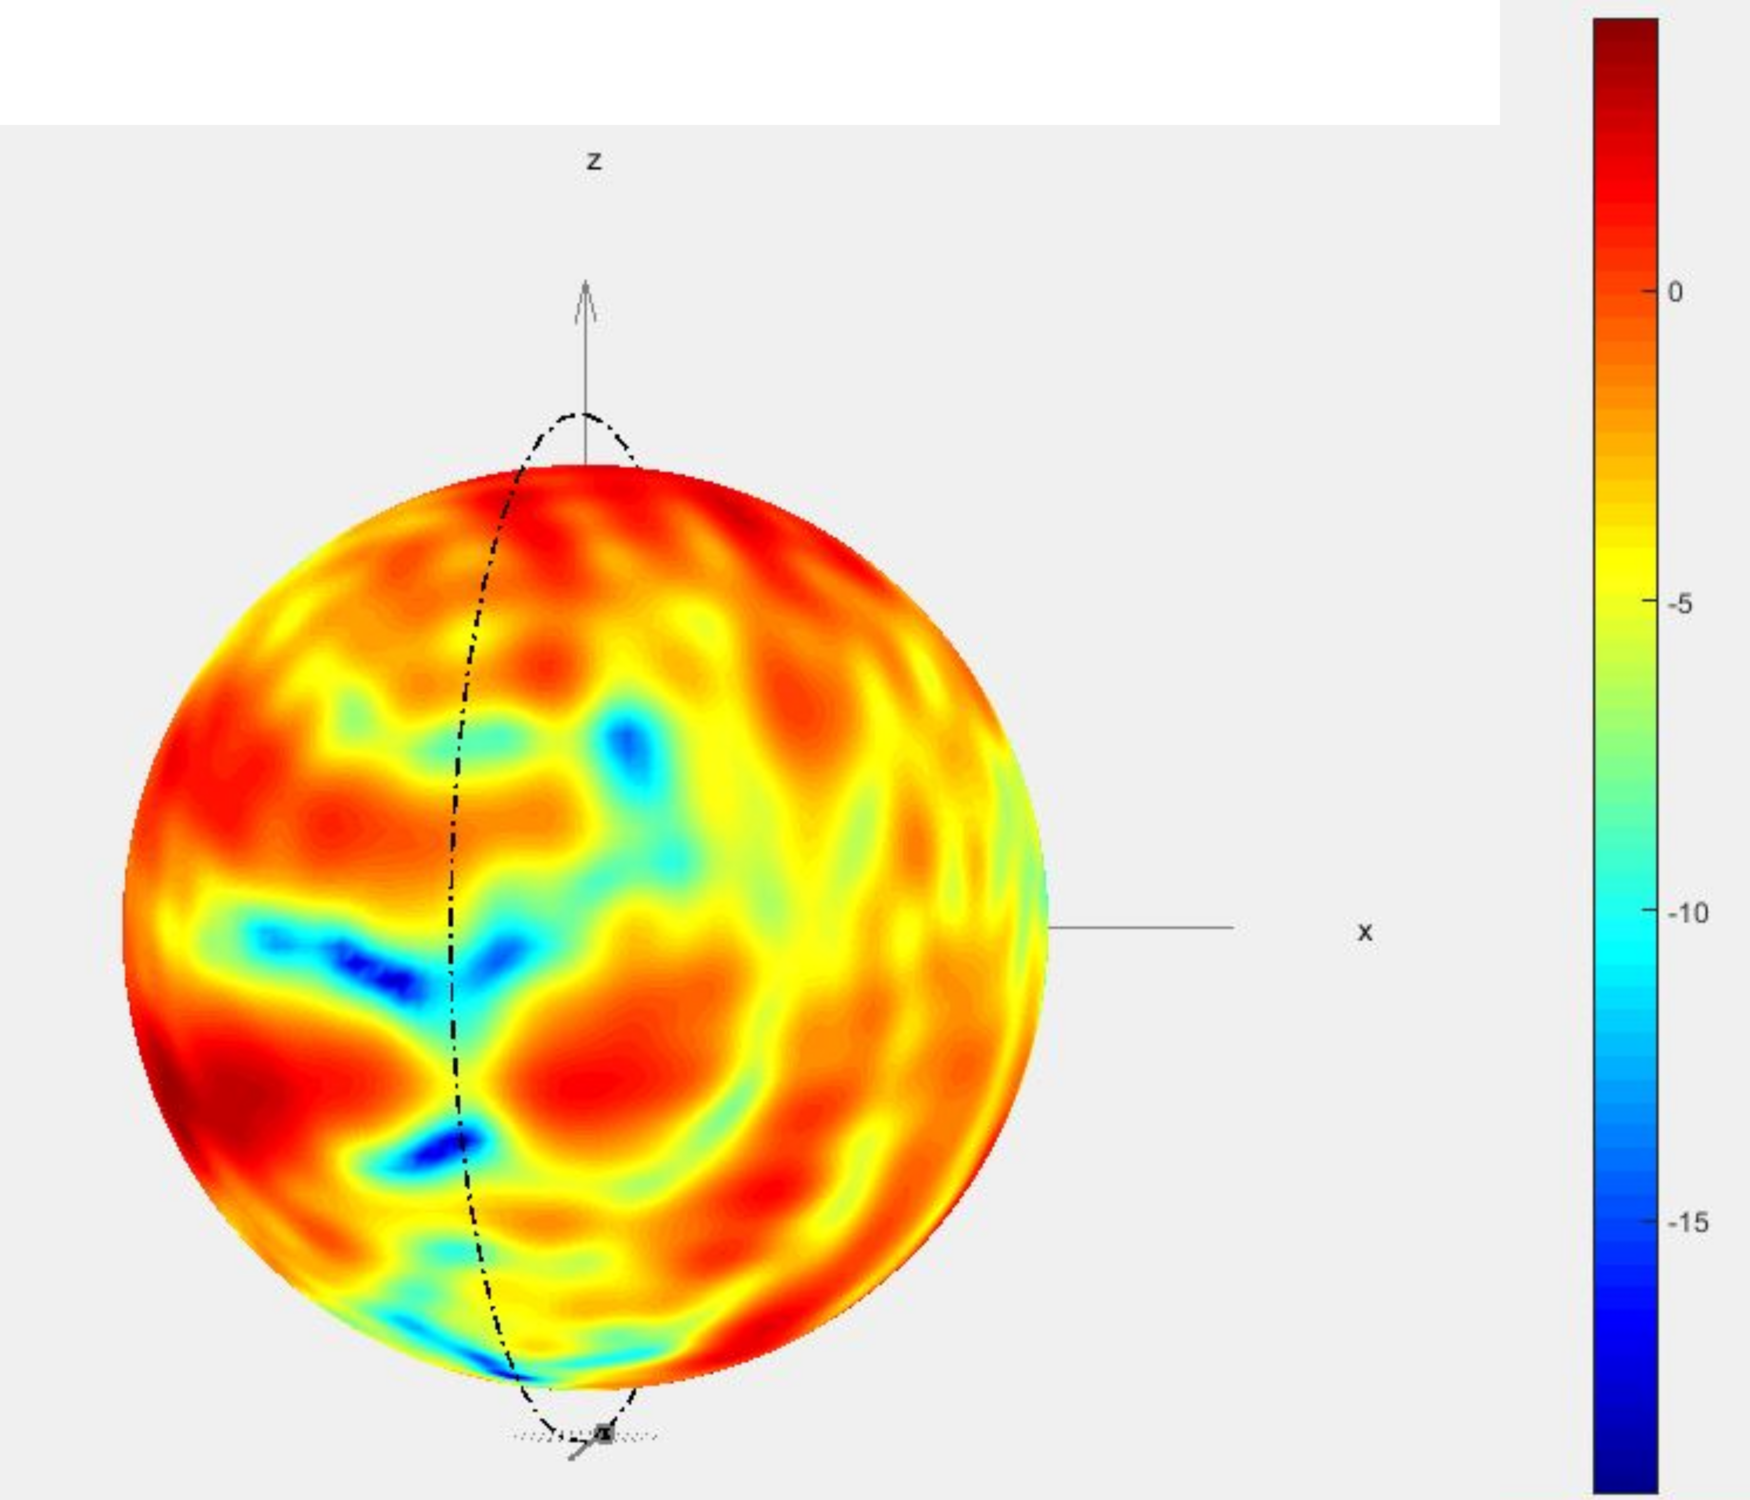
\includegraphics[width=1\textwidth]{../fig/plt/star_lab_5ghz0_xz_reduced.png}
			\caption{$\vec{E_{tot}}$XZ \SI{5.0}{\giga\hertz}}
		\end{center}
	\end{subfigure}

	\begin{subfigure}[t]{0.35\textwidth}
		\begin{center}
			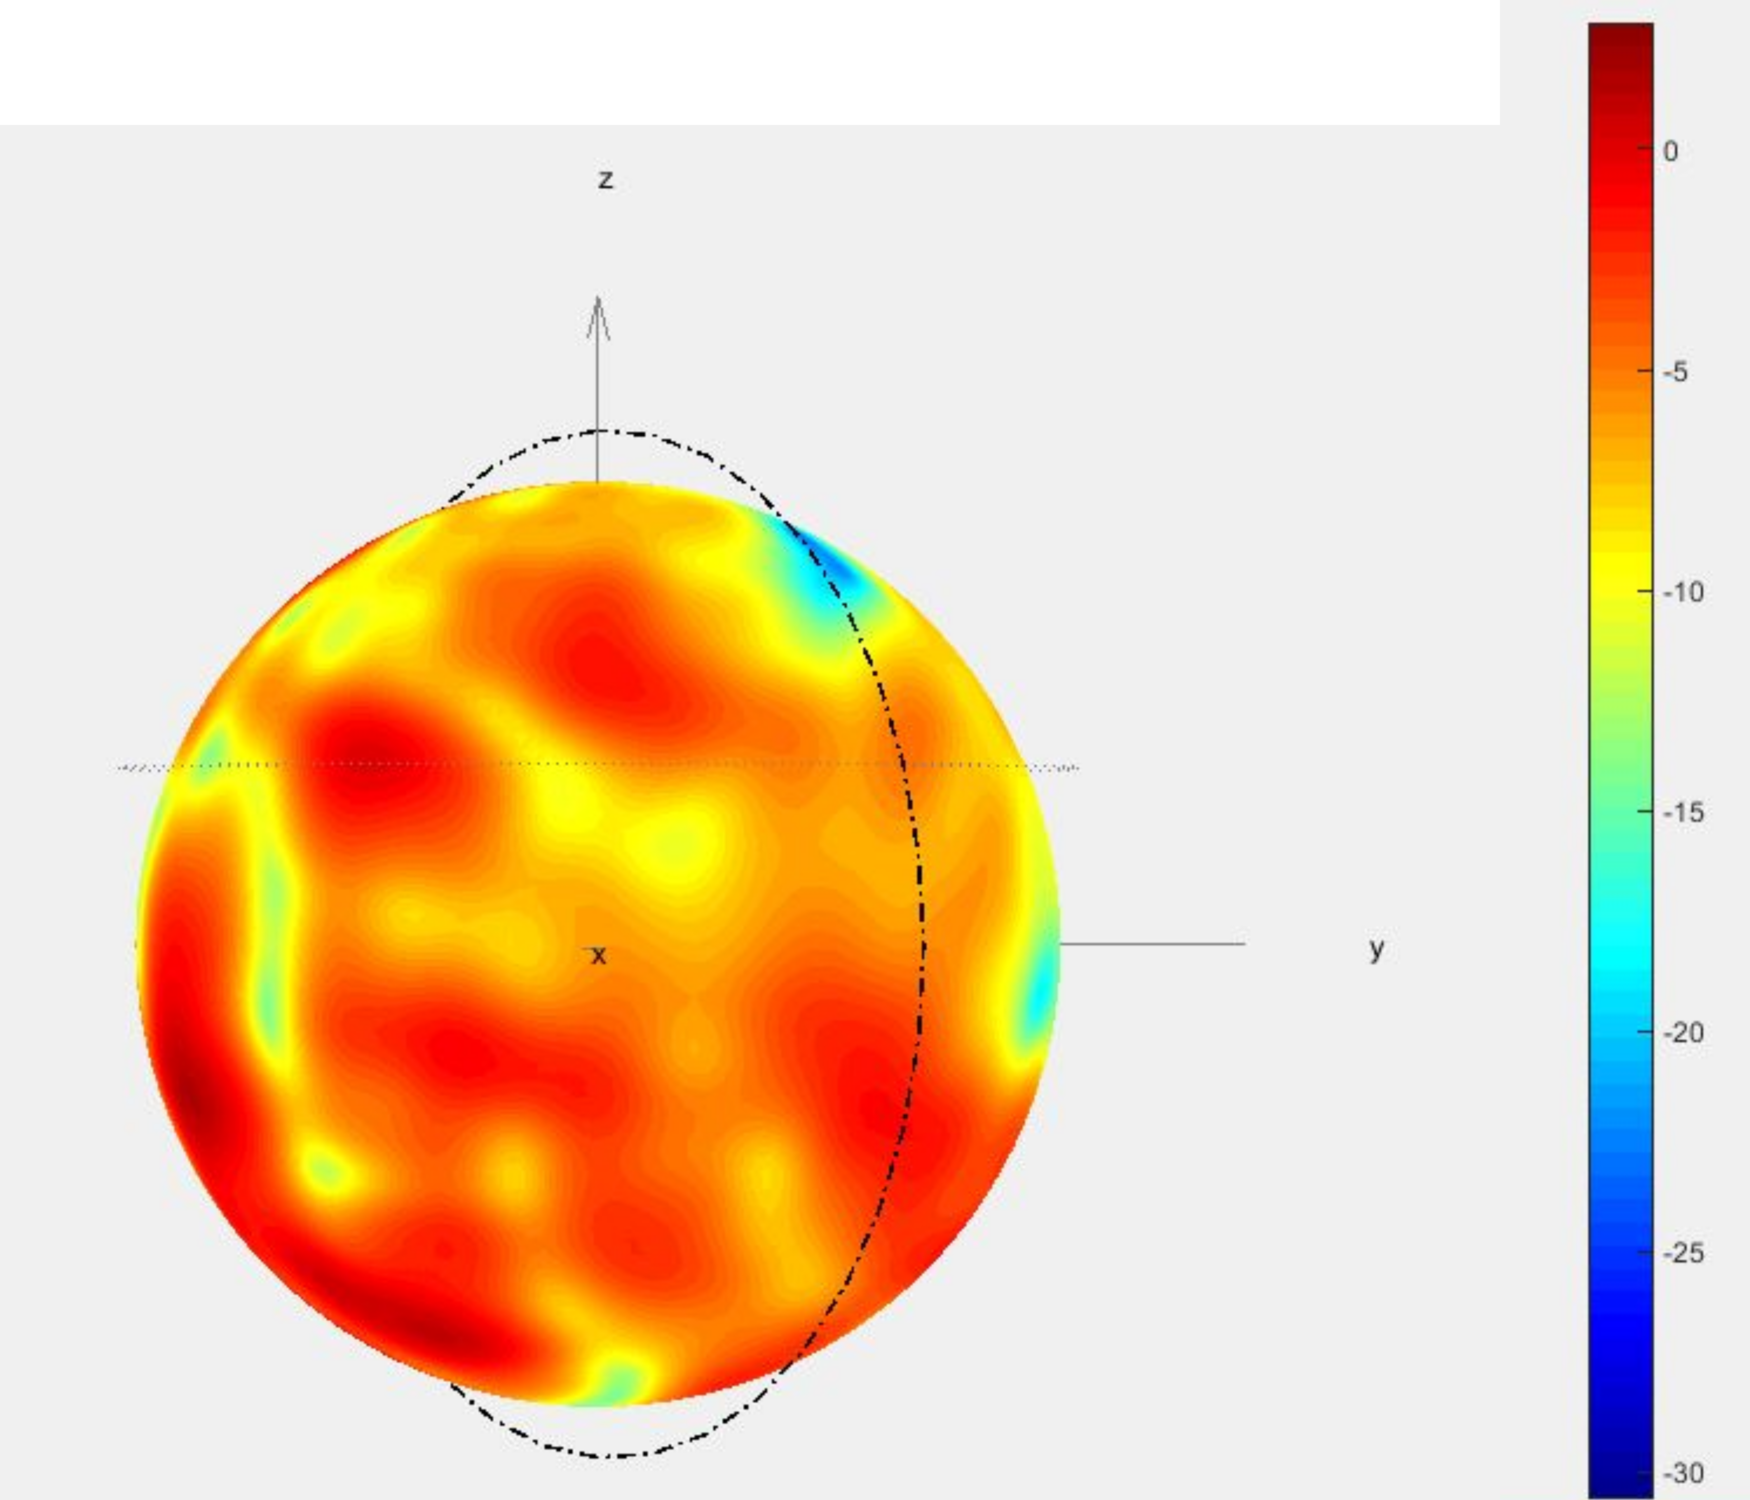
\includegraphics[width=1\textwidth]{../fig/plt/star_lab_2ghz4_yz_reduced.png}
			\caption{$\vec{E_{tot}}$YZ \SI{2.4}{\giga\hertz}}
		\end{center}
	\end{subfigure}
	\begin{subfigure}[t]{0.35\textwidth}
		\begin{center}
			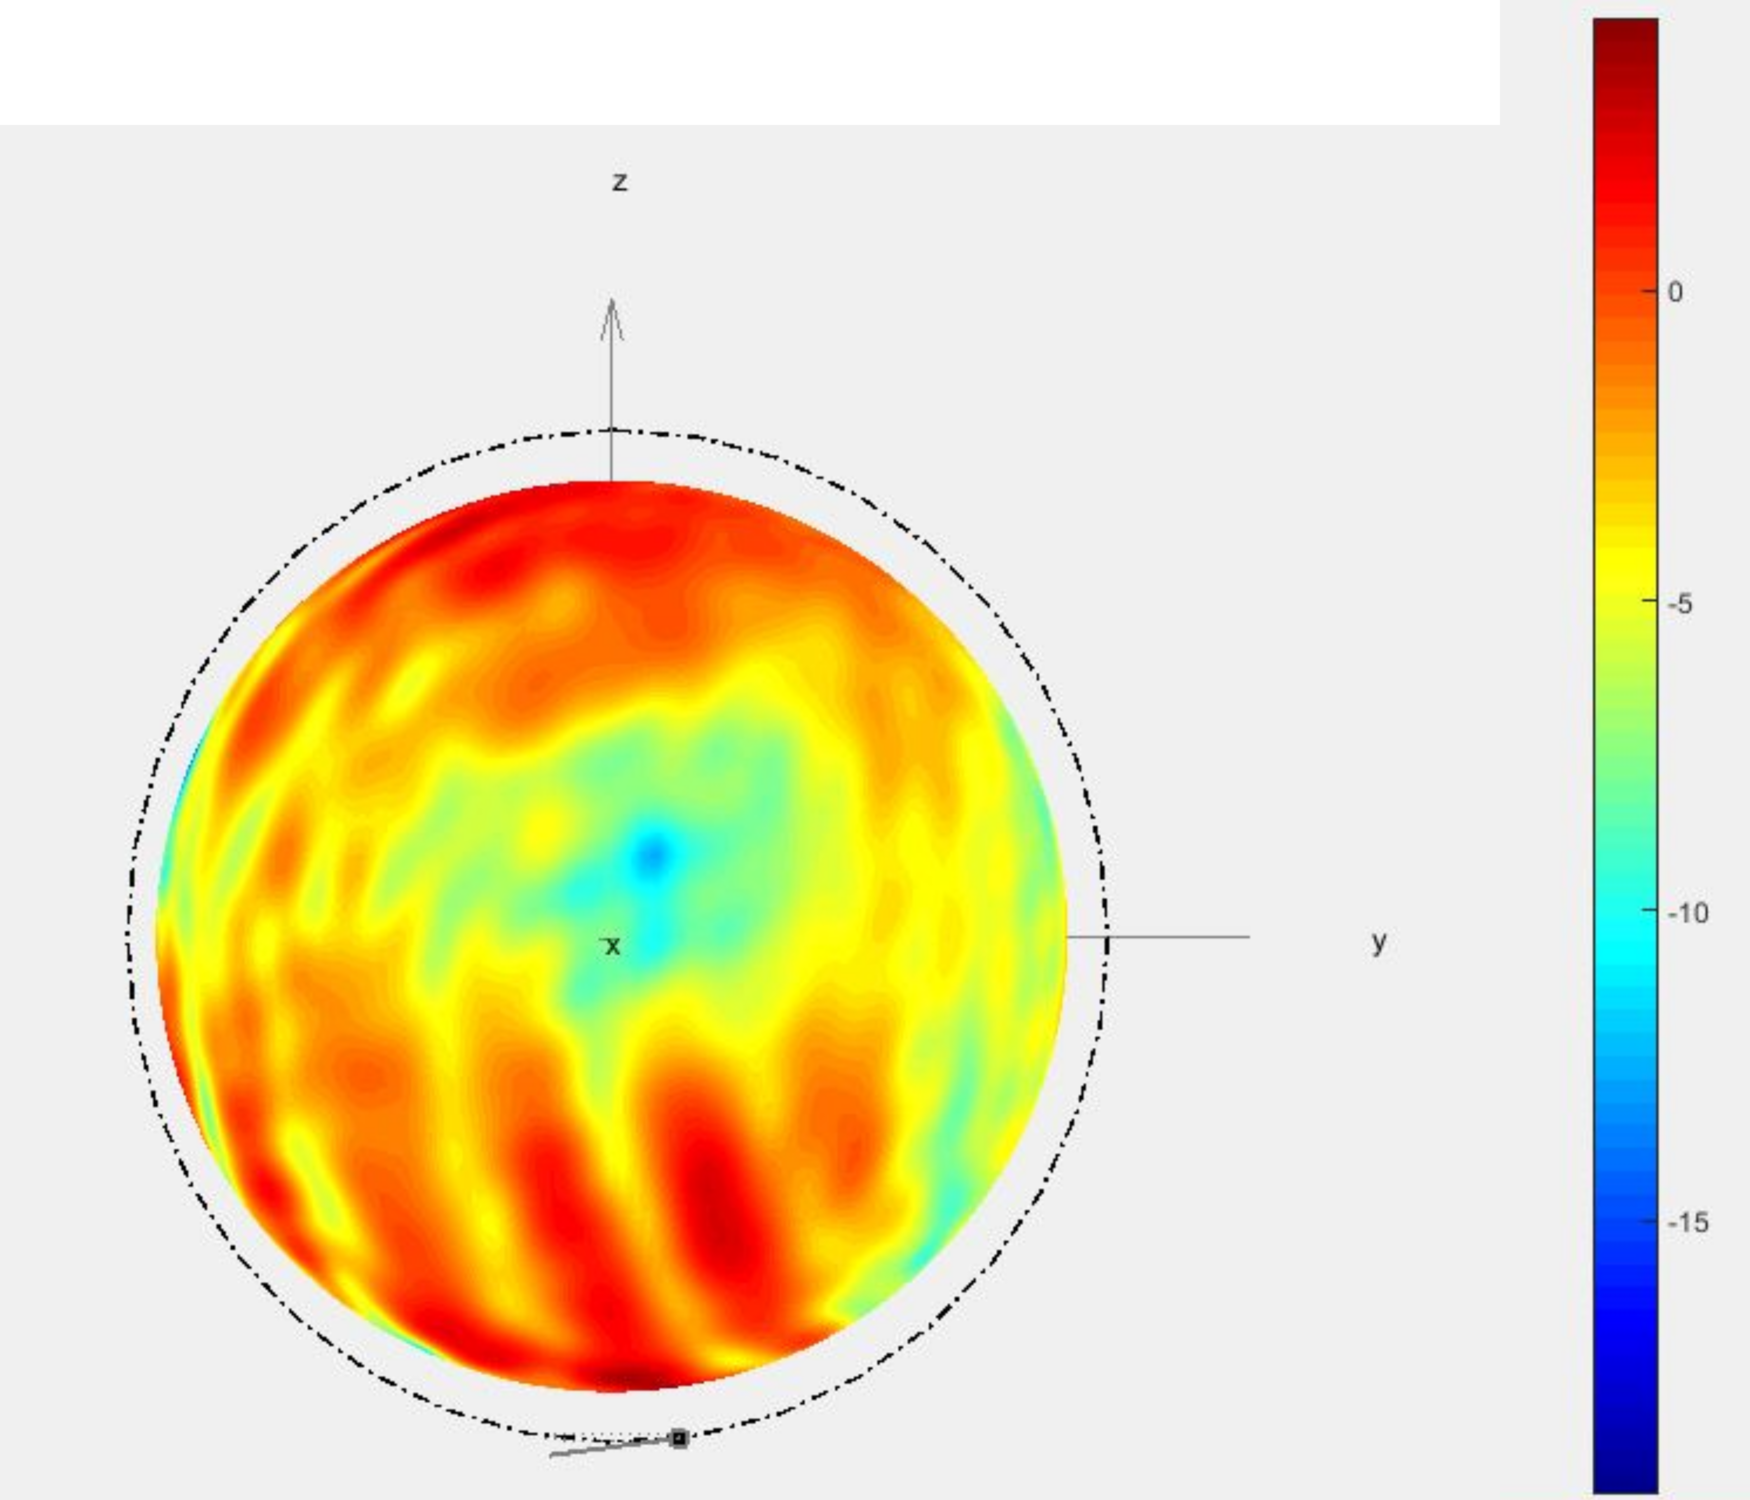
\includegraphics[width=1\textwidth]{../fig/plt/star_lab_5ghz0_yz_reduced.png}
			\caption{$\vec{E_{tot}}$YZ \SI{5.0}{\giga\hertz}}
		\end{center}
	\end{subfigure}
	\caption[3D Abstrahlung gemessen mit StarLab]{
		3D Abstrahlung gemessen mit StarLab. Die Abbildung
		zeigt die Abstrahlung als eingefärbte Kugeln in den
		drei Grundansichten XY, XZ und YZ für die beiden
		Frequenzen \SI{2.4}{\giga\hertz} und
		\SI{5.0}{\giga\hertz}.}
\end{figure}

%\clearpage
%\begin{figure}[h!]
%	\begin{center}
%		\begin{subfigure}[t]{0.49\textwidth}
%			\begin{center}
%				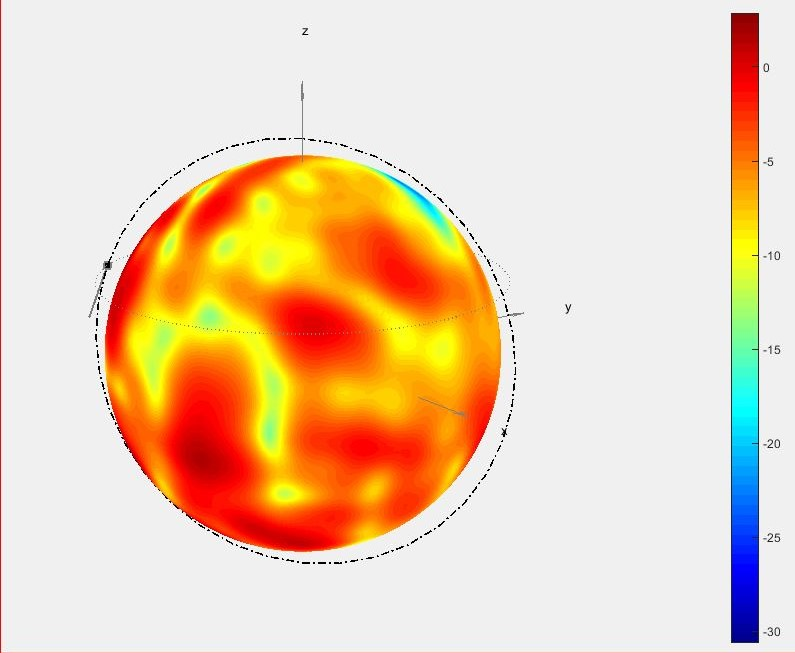
\includegraphics[width=1\textwidth]{../fig/plt/2_4GHz_justsphere.jpg}
%				\caption{Kugel 2.4 GHz}
%				\label{fig:sphere_2ghz4}
%			\end{center}
%		\end{subfigure}
%		\begin{subfigure}[t]{0.49\textwidth}
%			\begin{center}
%				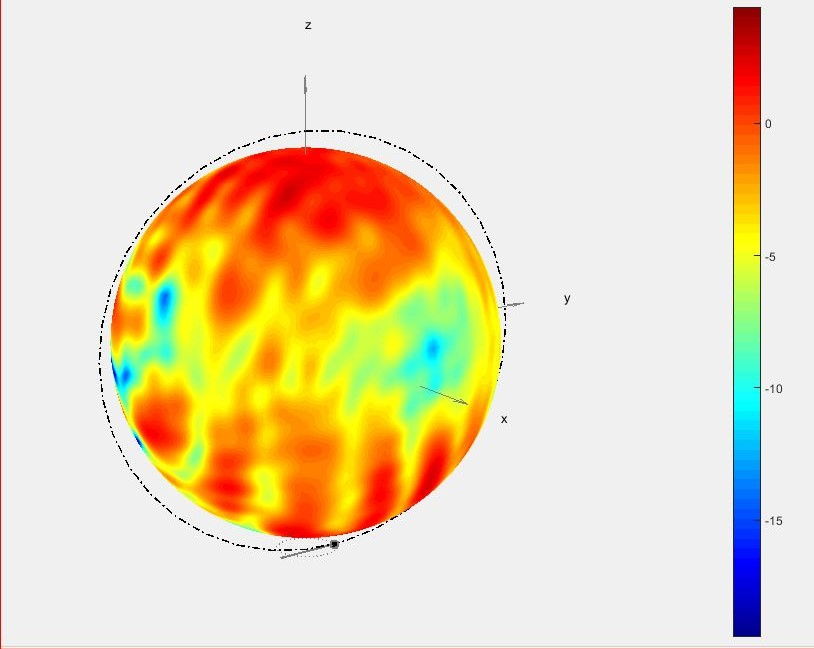
\includegraphics[width=1\textwidth]{../fig/plt/5GHz_just_sphere.jpg}
%				\caption{Kugel 5.0 GHz}
%				\label{fig:sphere_5ghz0}
%			\end{center}
%		\end{subfigure}
%		\caption{Starlab Messung Etot}
%		\label{fig:starlab_etot_sphere}
%	\end{center}
%\end{figure}

\clearpage
\subsubsection{Abstrahlung 1D}


\begin{figure}[h!]
	\centering
	\begin{subfigure}[b]{0.48\textwidth}
		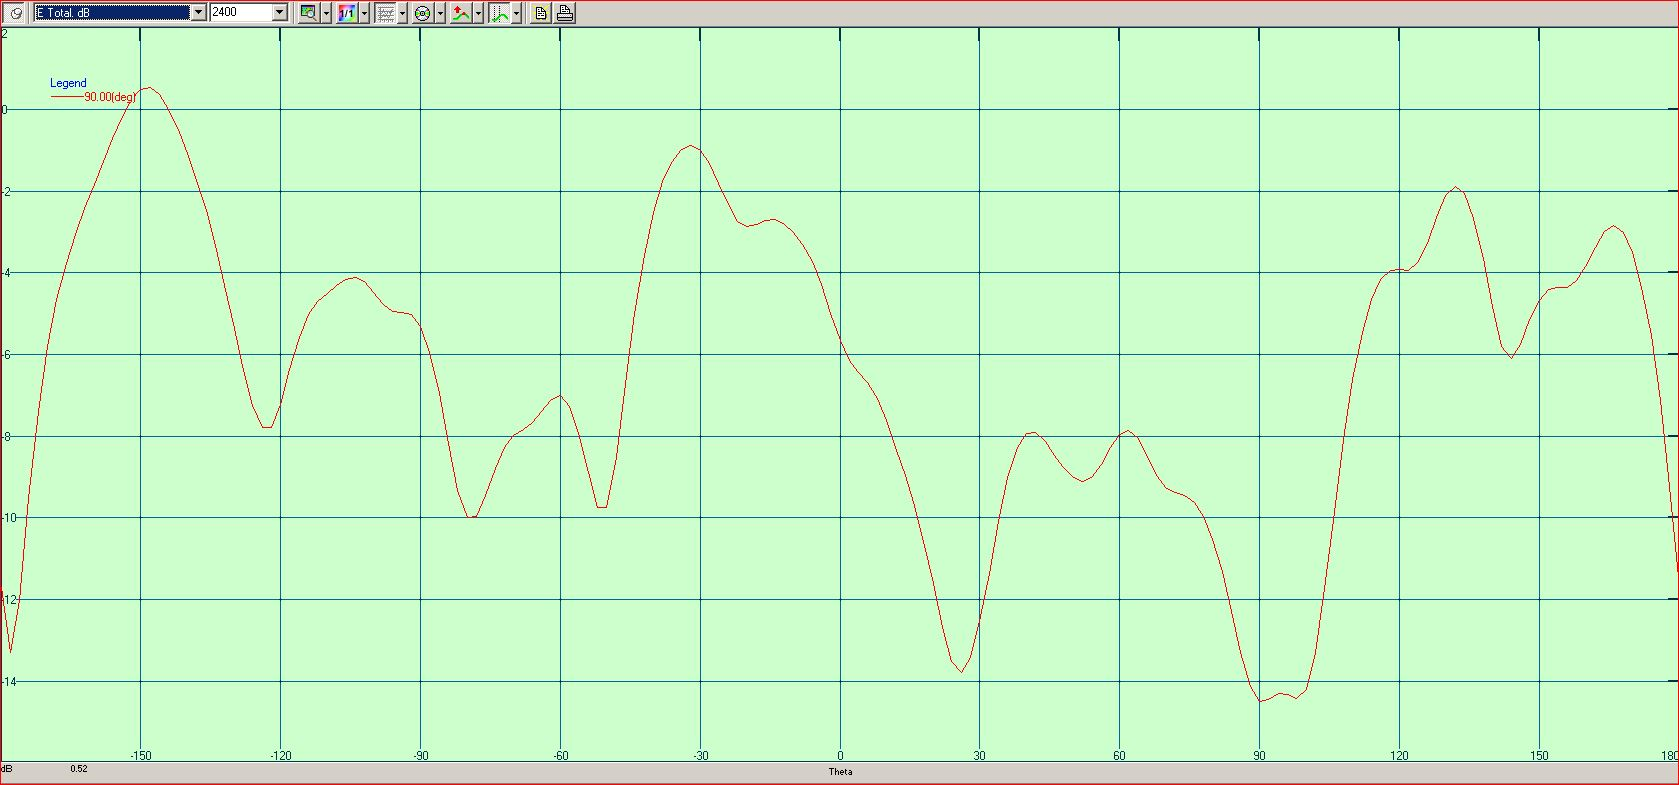
\includegraphics[width=1\textwidth]{../fig/plt/2G4_90phi_etot_dB.JPG}
		\caption{$\vec{E_{tot}}$ mit $\varphi=\SI{90}{\degree}$ bei \SI{2.4}{\giga\hertz}}
	\end{subfigure}
	\begin{subfigure}[b]{0.48\textwidth}
		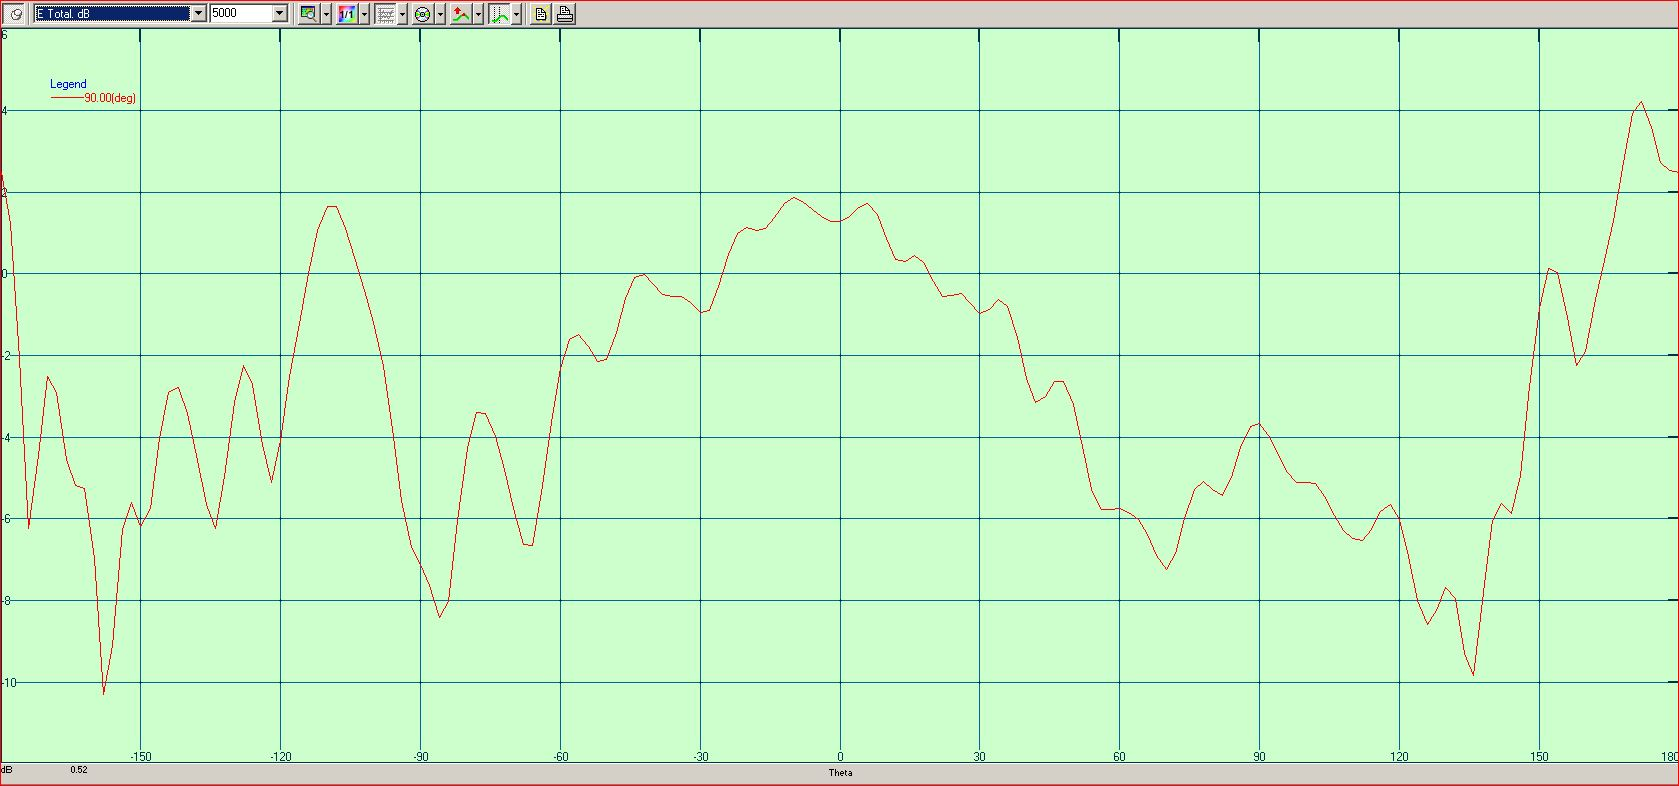
\includegraphics[width=1\textwidth]{../fig/plt/5G0_90phi_etot_dB.JPG}
		\caption{$\vec{E_{tot}}$ mit $\varphi=\SI{90}{\degree}$ bei \SI{5.0}{\giga\hertz}}
	\end{subfigure}

	\begin{subfigure}[b]{0.48\textwidth}
		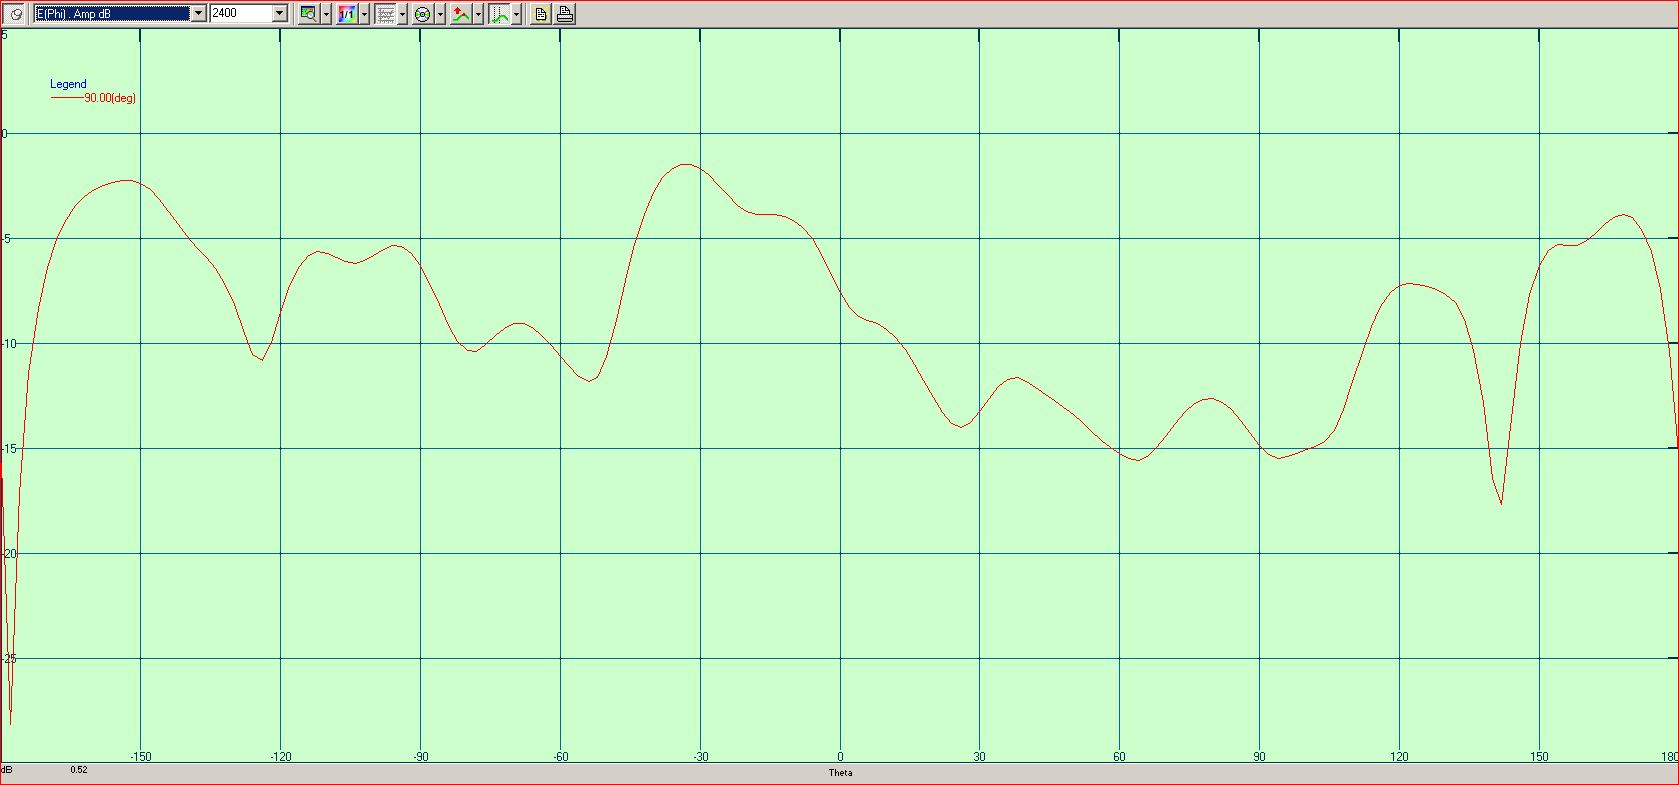
\includegraphics[width=1\textwidth]{../fig/plt/2G4_90phi_ephi_amp_dB.JPG}
		\caption{$\vec{E_{\varphi}}$ mit $\varphi=\SI{90}{\degree}$ bei \SI{2.4}{\giga\hertz}}
	\end{subfigure}
	\begin{subfigure}[b]{0.48\textwidth}
		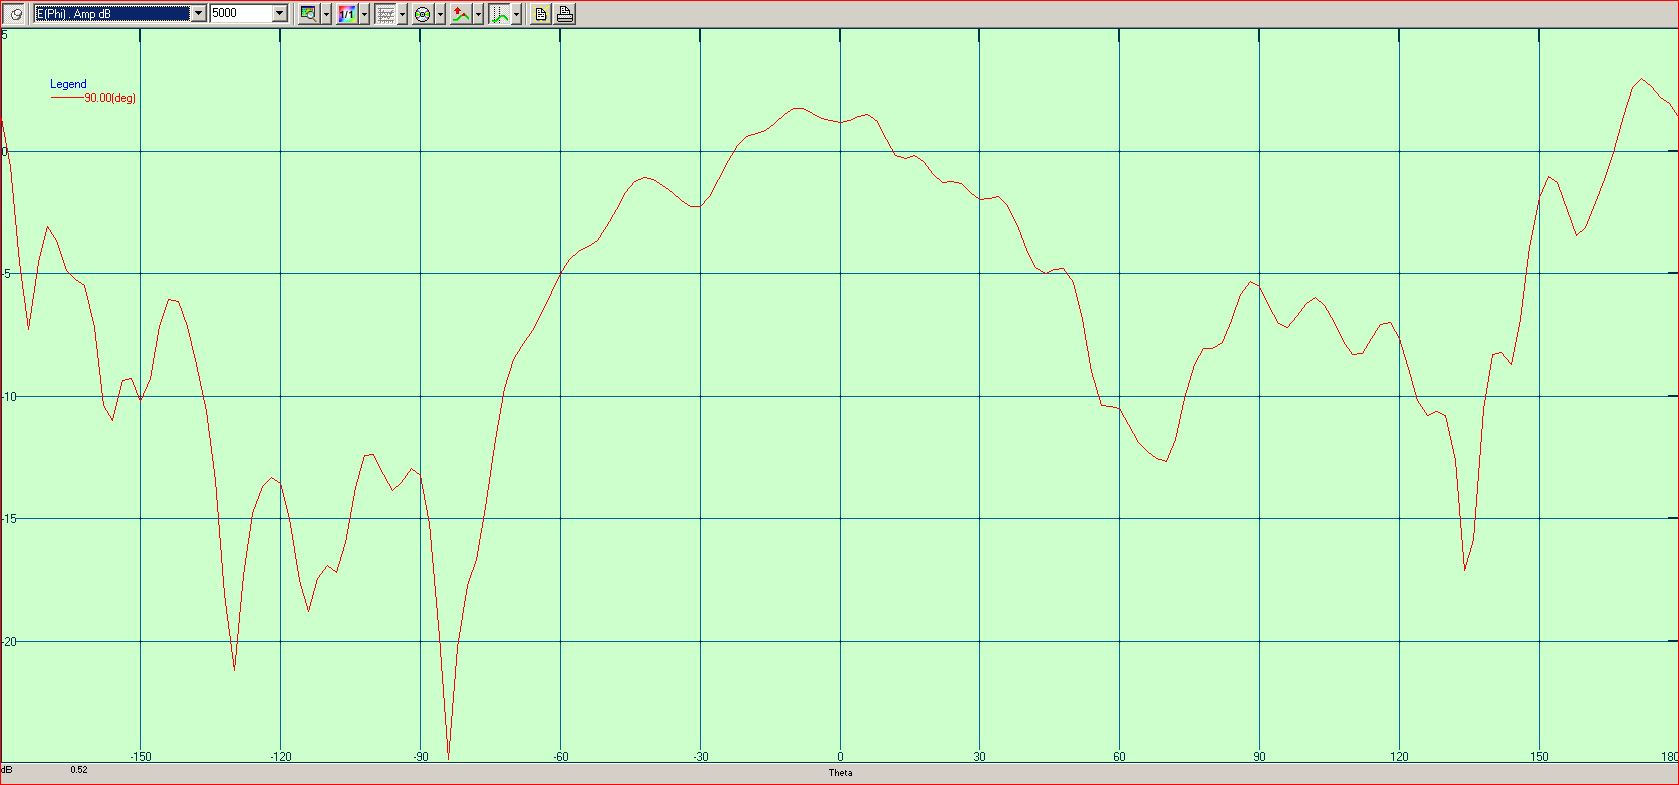
\includegraphics[width=1\textwidth]{../fig/plt/5G0_90phi_ephi_amp_dB.JPG}
		\caption{$\vec{E_{\varphi}}$ mit $\varphi=\SI{90}{\degree}$ bei \SI{5.0}{\giga\hertz}}
	\end{subfigure}

	\begin{subfigure}[b]{0.48\textwidth}
		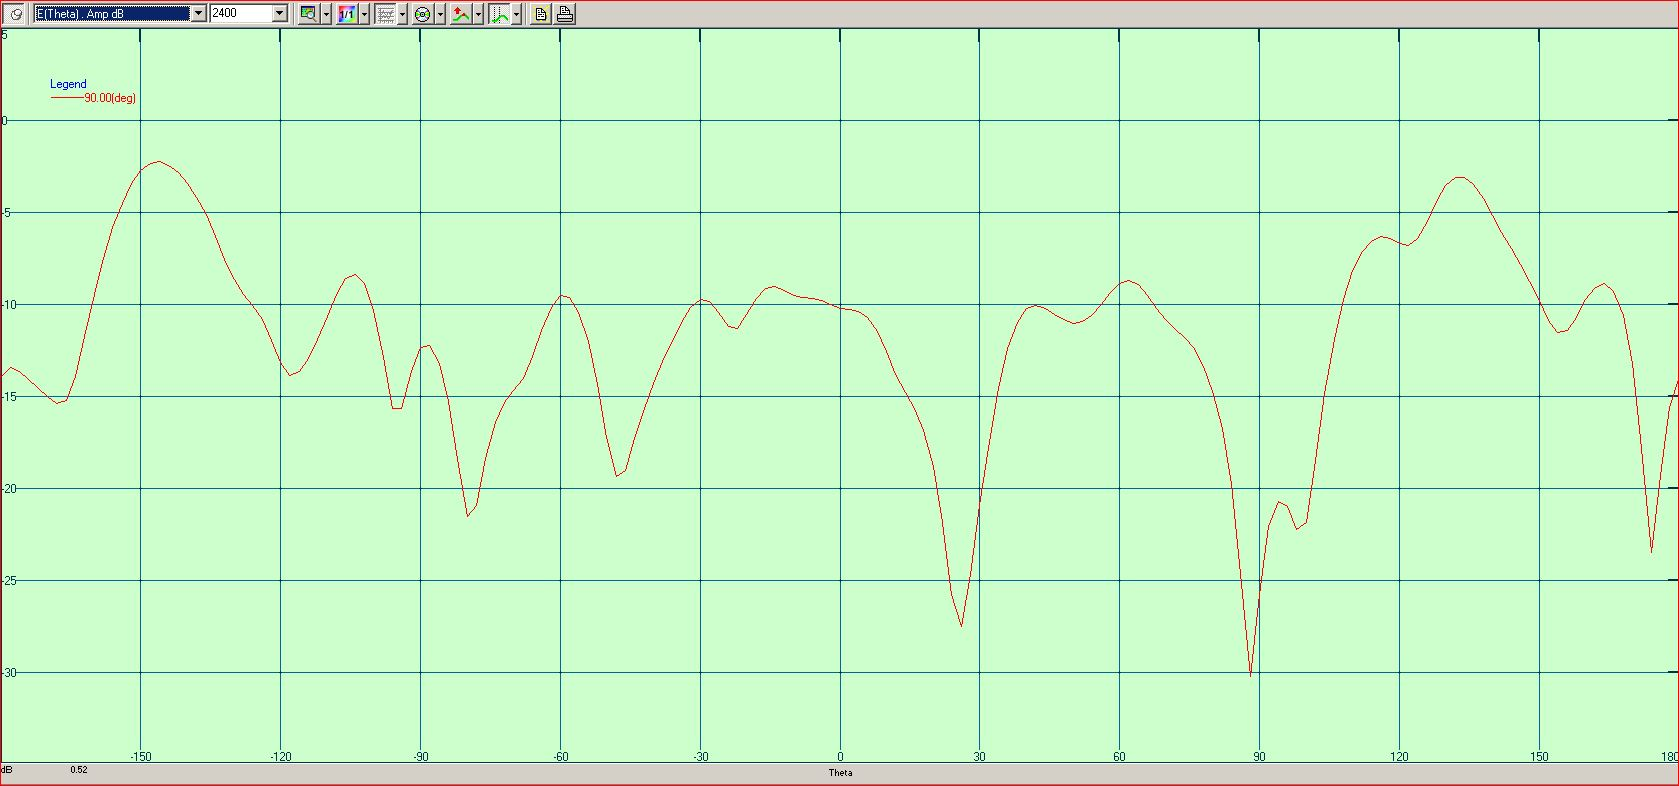
\includegraphics[width=1\textwidth]{../fig/plt/2G4_90phi_etheta_amp_dB.JPG}
		\caption{$\vec{E_{\theta}}$ mit $\varphi=\SI{90}{\degree}$ bei \SI{2.4}{\giga\hertz}}
	\end{subfigure}
	\begin{subfigure}[b]{0.48\textwidth}
		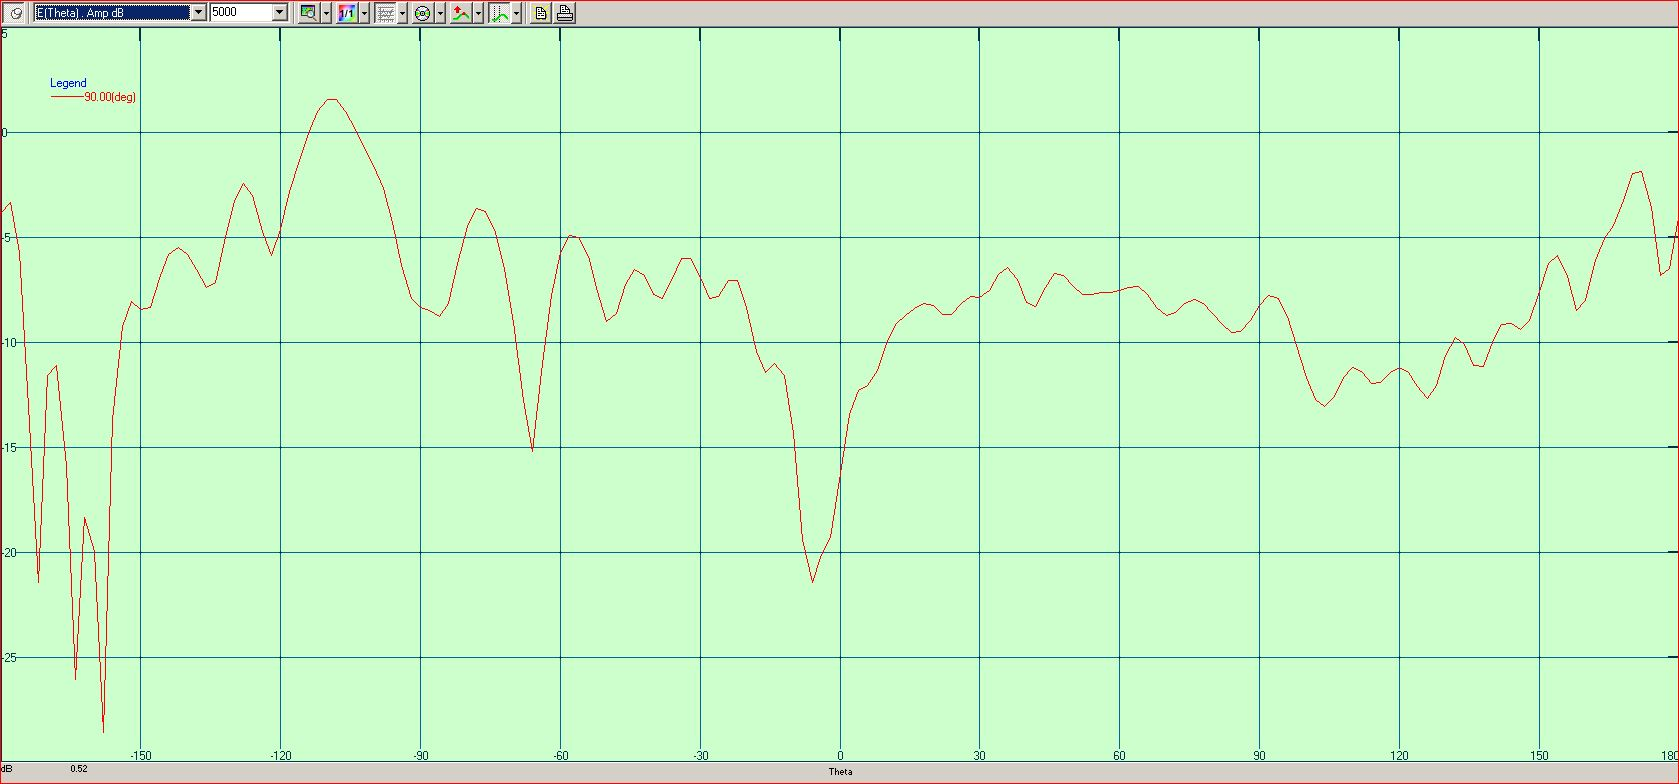
\includegraphics[width=1\textwidth]{../fig/plt/5G0_90phi_etheta_amp_dB.JPG}
		\caption{$\vec{E_{\theta}}$ mit $\varphi=\SI{90}{\degree}$ bei \SI{5.0}{\giga\hertz}}
	\end{subfigure}
	\caption[1D Messungen mit StarLab für $\vec{E_{tot}}$, $\vec{E_{\varphi}}$ und $\vec{E_{\theta}}$]{
		1D Messungen mit StarLab für $\vec{E_{tot}}$, $\vec{E_{\varphi}}$ und $\vec{E_{\theta}}$.
		Die Abbildung zeigt die gemessenen Verläufe für die
		verschiedenen Vektoren bei fixiertem
		$\varphi = \SI{90}{\degree}$.}
\end{figure}



%\begin{figure}[h!]
%	\begin{center}
%		\begin{subfigure}[t]{0.49\textwidth}
%			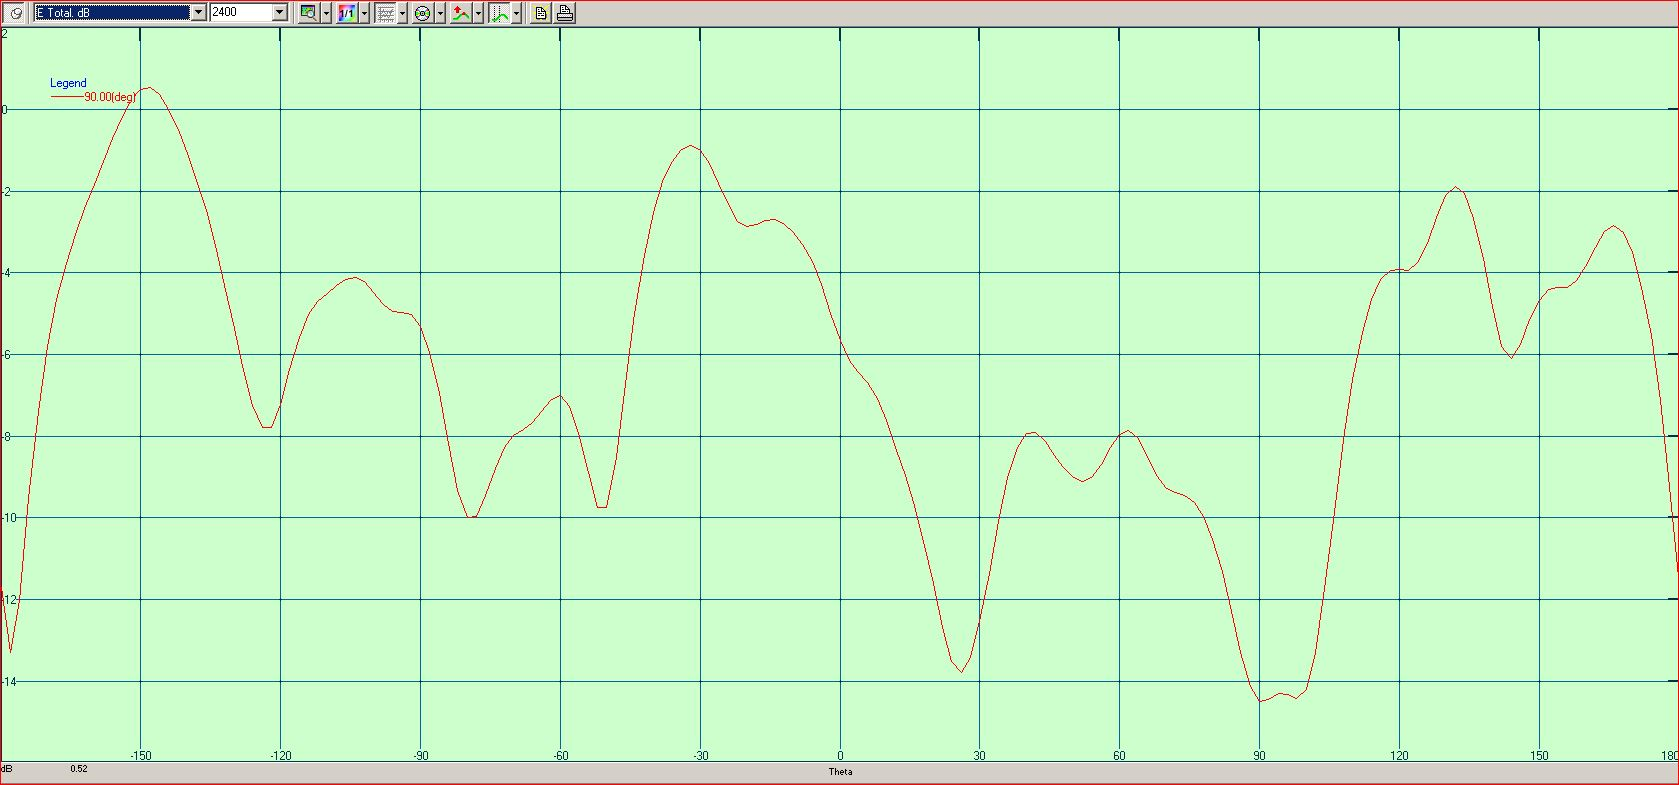
\includegraphics[width=1\textwidth]{../fig/plt/2G4_90phi_etot_dB.JPG}
%			\caption{\SI{2.4}{\giga\hertz}}
%		\end{subfigure}
%		\begin{subfigure}[t]{0.49\textwidth}
%			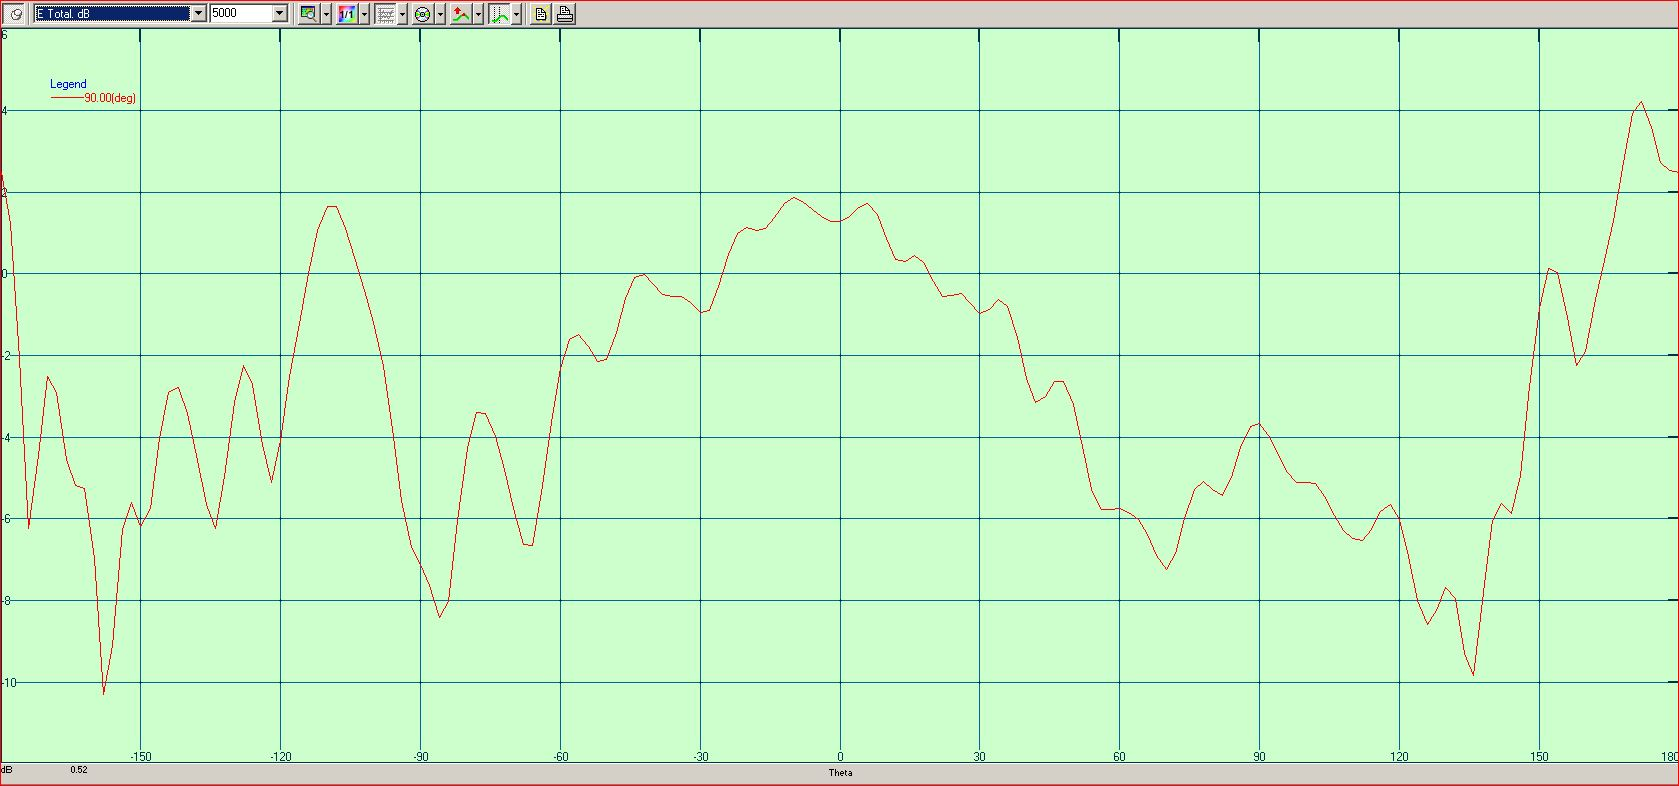
\includegraphics[width=1\textwidth]{../fig/plt/5G0_90phi_etot_dB.JPG}
%			\caption{\SI{5.0}{\giga\hertz}}
%		\end{subfigure}
%		\caption[Auswertung der Abstrahlungscharakteristik]{
%			Auswertung der Abstrahlungscharakteristik.
%			Die Abbildung zeigt die gemessenen Werte von $\vec{E}_{tot}$
%			bei fixiertem $\varphi = \SI{90}{\degree}$.}
%		\label{fig:starlab_etot_curve}
%	\end{center}
%\end{figure}
%
%\begin{figure}[h!]
%	\centering
%	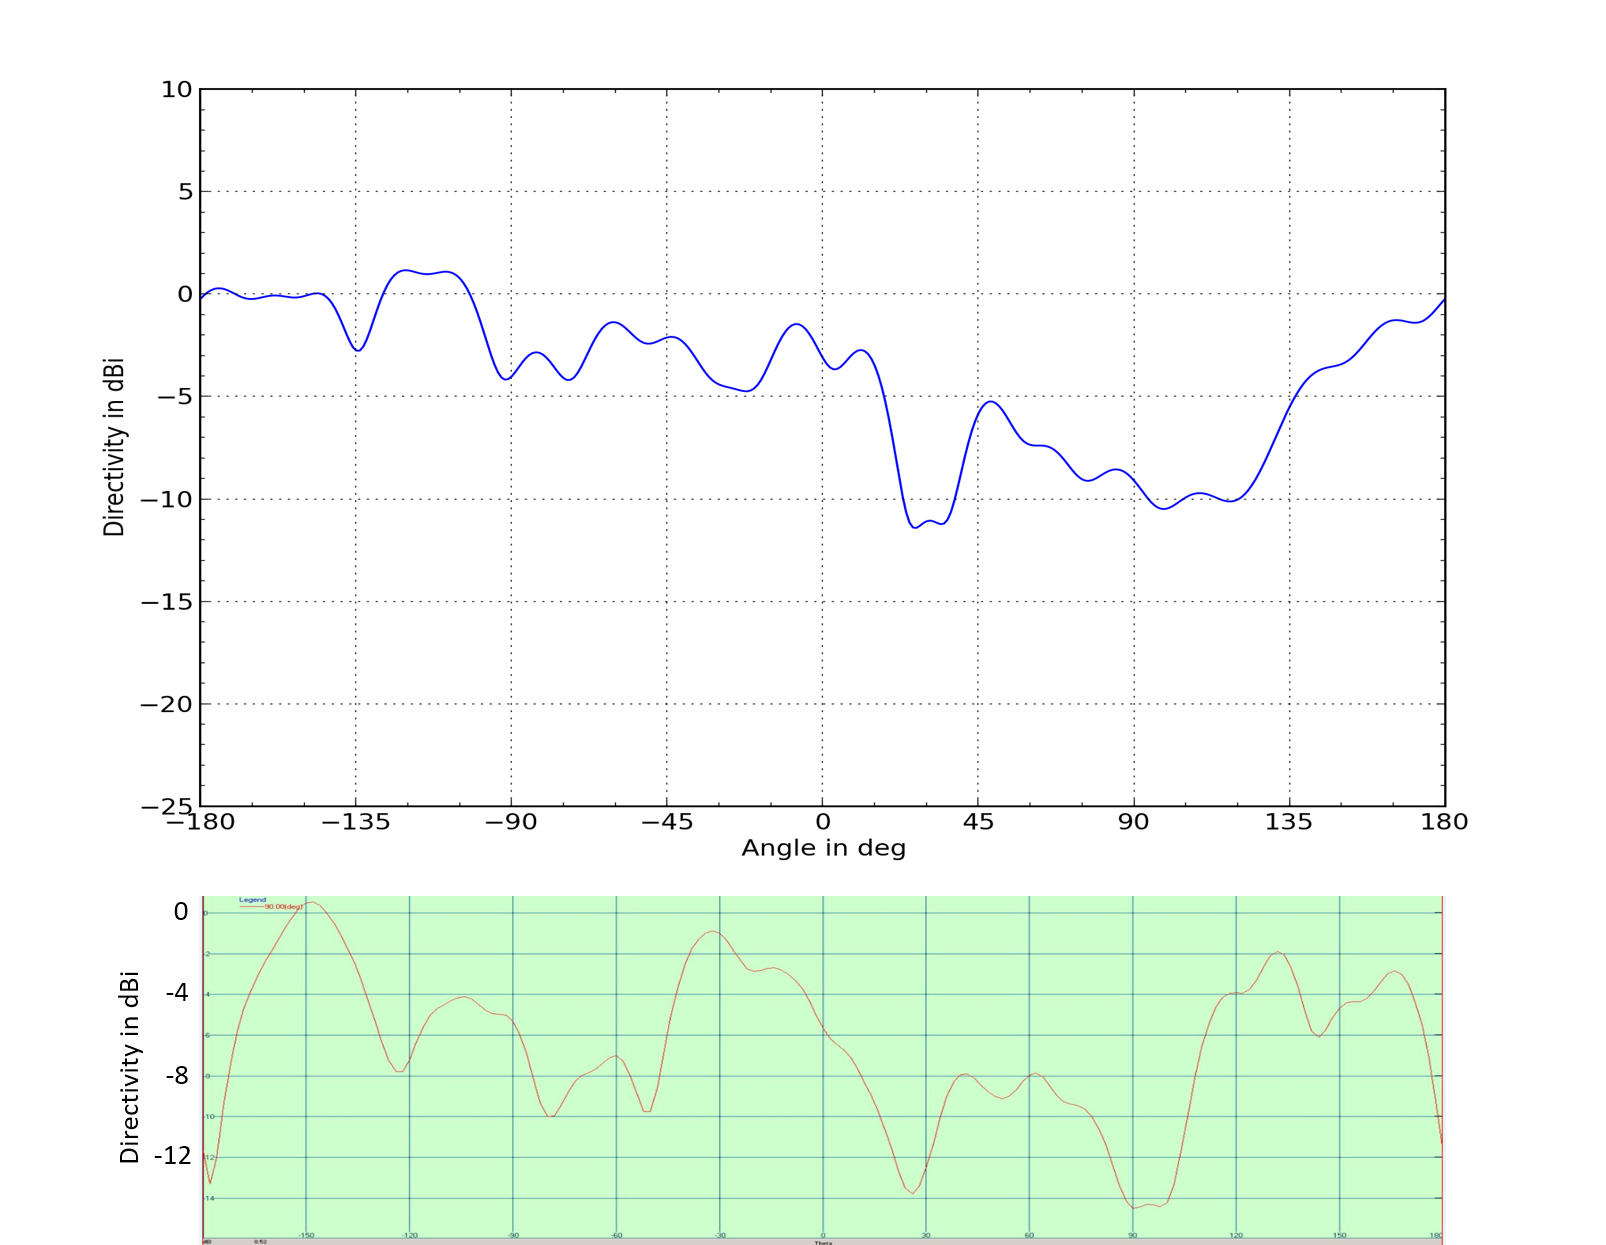
\includegraphics[width=0.8\textwidth]{../fig/plt/comparison_l4_pcb_v2c_laptop_1a_105_etot_phi90_2ghz4.png}
%	\caption{$\vec{E}_{\varphi}$ \;\; \SI{90}{\degree} \\
%		\hspace*{107pt}oben: simuliert\\
%		\hspace*{115pt}unten: gemessen}
%	\label{fig:E_tot_90}
%\end{figure}

\clearpage
\subsubsection{Optimale Abstrahlung}

\begin{figure}[h!]
	\begin{subfigure}[t]{0.49\textwidth}
		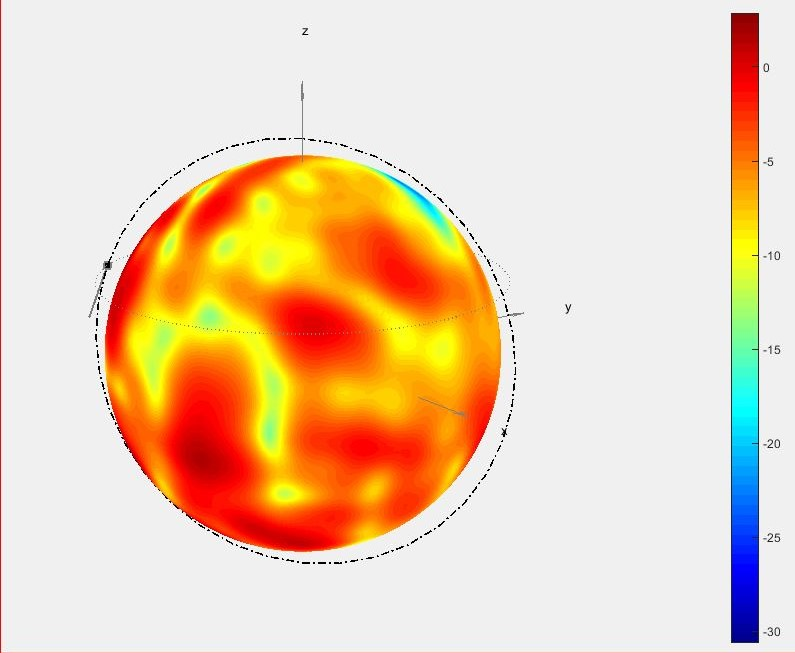
\includegraphics[width=1\textwidth]{../fig/plt/2_4GHz_justsphere.jpg}
		\caption{Kugel 2.4 GHz}
	\end{subfigure}
	\begin{subfigure}[t]{0.49\textwidth}
		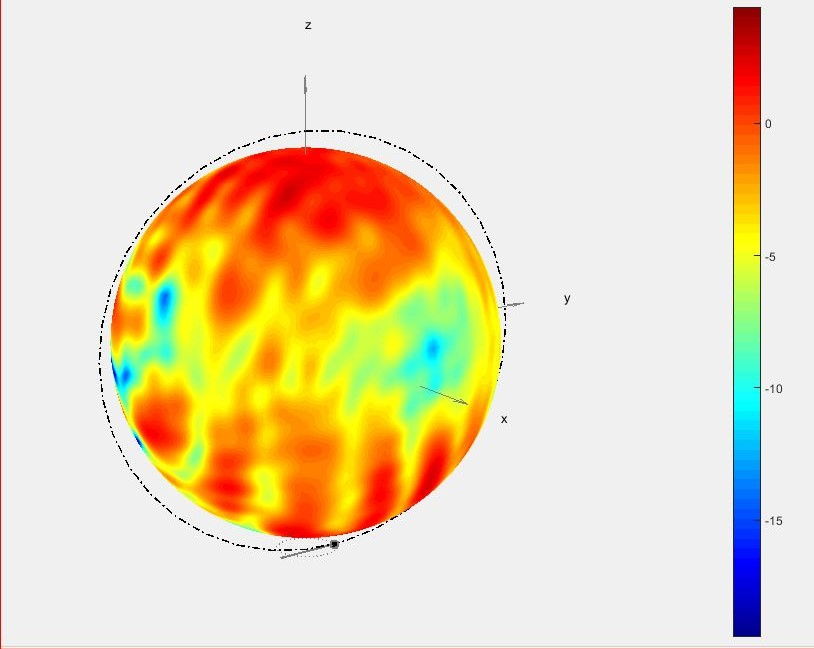
\includegraphics[width=1\textwidth]{../fig/plt/5GHz_just_sphere.jpg}
		\caption{Kugel 5.0 GHz}
	\end{subfigure}
	
	\begin{subfigure}[t]{0.49\textwidth}
		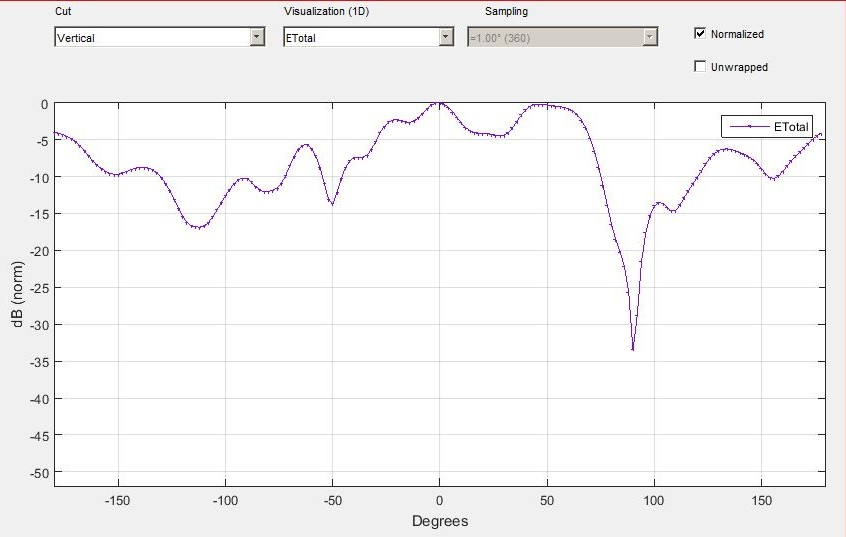
\includegraphics[width=1\textwidth]{../fig/plt/2_4GHz_E_tot_curve.jpg}
		\caption{Kurve 2.4 GHz}
	\end{subfigure}
	\begin{subfigure}[t]{0.49\textwidth}
		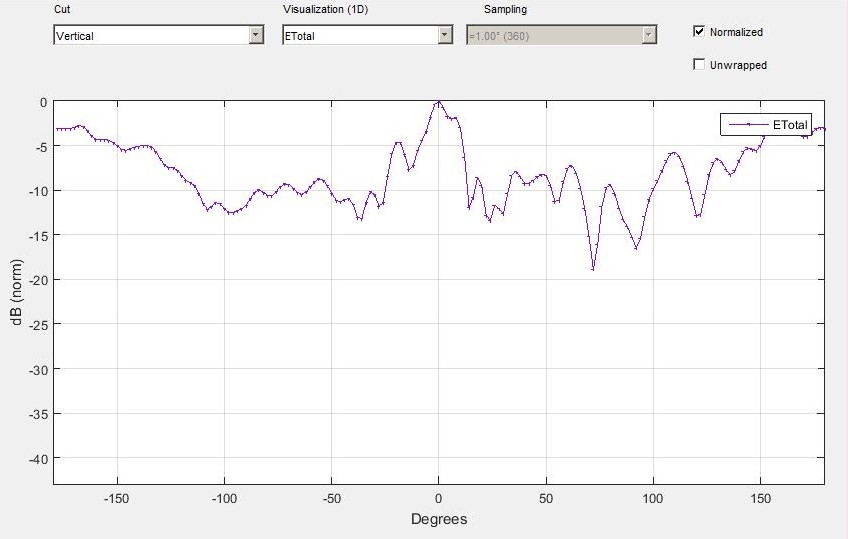
\includegraphics[width=1\textwidth]{../fig/plt/5GHz_E_tot_curve.jpg}
		\caption{Kurve 5.0 GHz}
	\end{subfigure}
	\caption[Optimale Abstrahlung ausgewertet mit dem Antenna Analyser]{
		Optimale Abstrahlung ausgewertet mit dem Antenna Analyser.
		Die Abbildung zeigt den jeweiligen Punkt mit optimaler
		Abstrahlung für \SI{2.4}{\giga\hertz} und \SI{5.0}{\giga\hertz}
		als schwarzen Punkt in den 3D Darstellungen (a,b). Der durch den
		jeweiligen Punkt verlaufende Ring (gestrichtelt) zeigt die
		ausgewertete Abstrahlung, welche als eindimensionaler Verlauf
		von $\vec{E_{tot}}$ dargestellt ist (c,d).}
	\label{fig:etot_max_measured}
\end{figure}

Die optimale Abstrahlung wurde mit dem Antenna Analyser ermittelt.
Die Abbildung \ref{fig:etot_max_measured} zeigt die dabei festgestellten
Ergebnisse.

\clearpage
\section{Vergleich Simulation und Messung}

\subsection{Abstrahlung 3D}

\begin{figure}[h!]
	\centering
	\begin{subfigure}[b]{0.48\textwidth}
		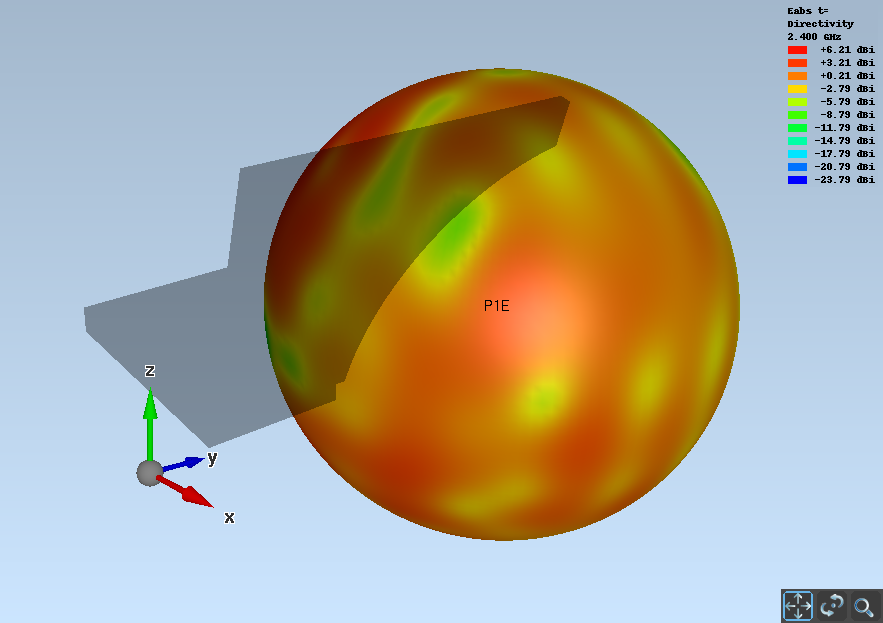
\includegraphics[width=1\textwidth]{../fig/plt/crazy_stuff_l4_pcb_v2c_laptop_1a_105_2ghz4_3d_eabs_sphere.png}
		\caption{Simulation \SI{2.4}{\giga\hertz}}
	\end{subfigure}
	\begin{subfigure}[b]{0.48\textwidth}
		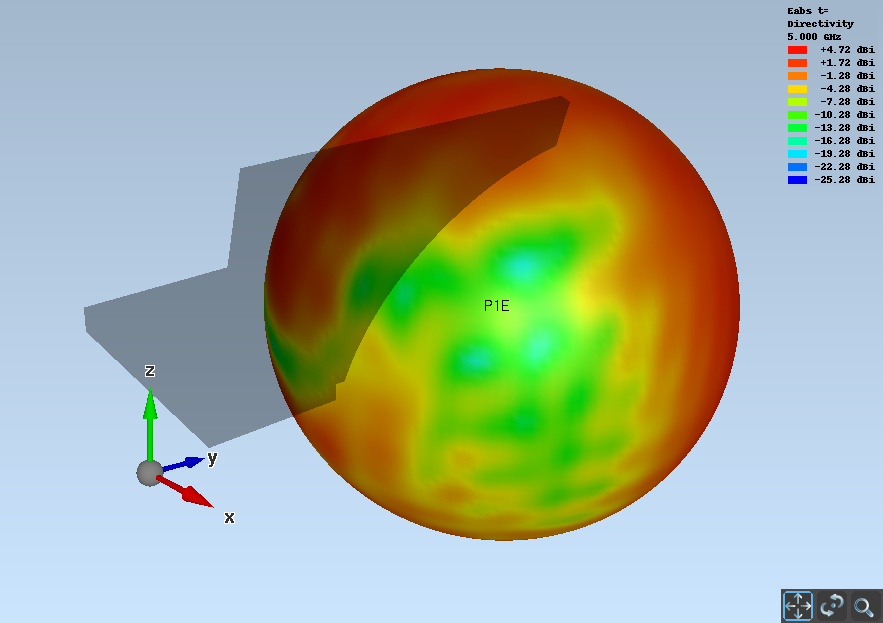
\includegraphics[width=1\textwidth]{../fig/plt/crazy_stuff_l4_pcb_v2c_laptop_1a_105_5ghz_3d_eabs_sphere.png}
		\caption{Simulation \SI{5.0}{\giga\hertz}}
	\end{subfigure}

	\begin{subfigure}[t]{0.49\textwidth}
	 	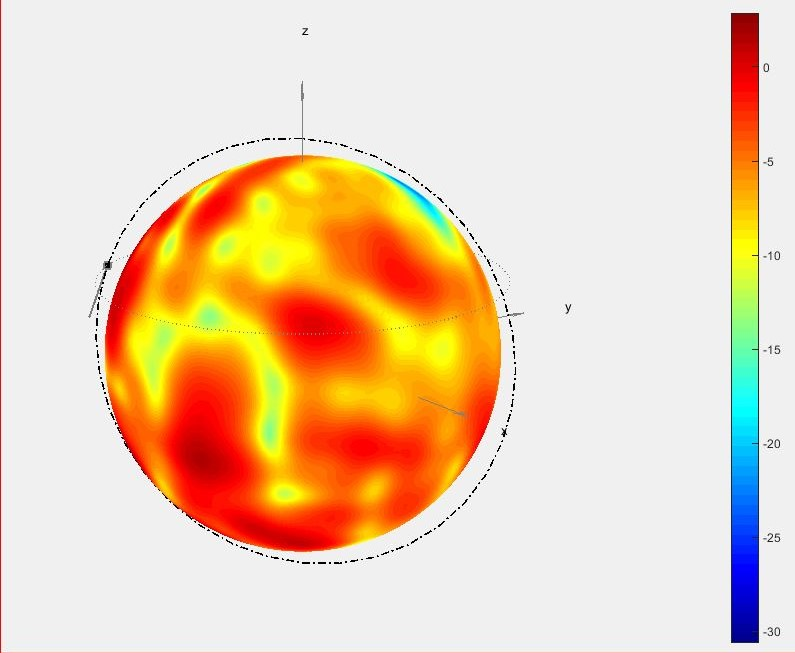
\includegraphics[width=1\textwidth]{../fig/plt/2_4GHz_justsphere.jpg}
		\caption{Messung \SI{2.4}{\giga\hertz}}
	\end{subfigure}
	\begin{subfigure}[t]{0.49\textwidth}
		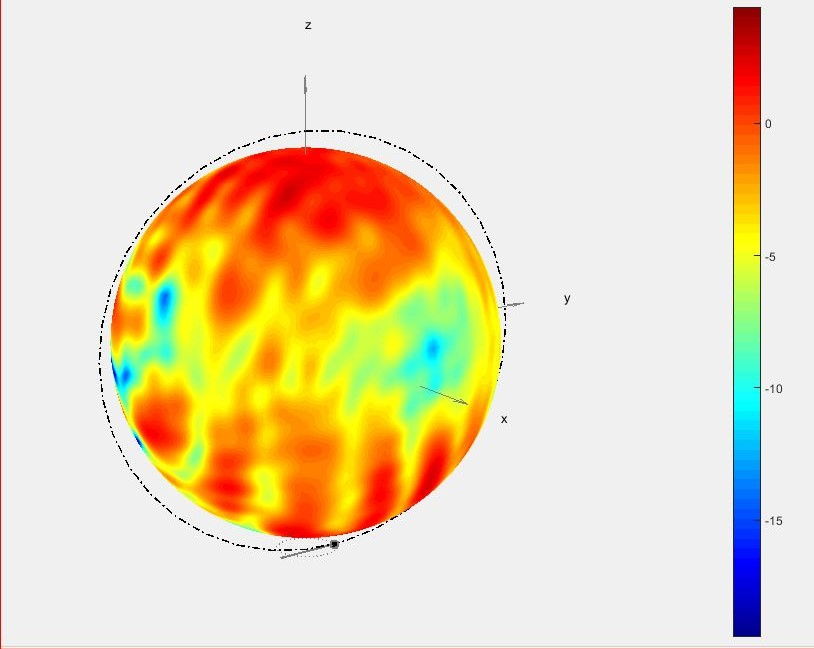
\includegraphics[width=1\textwidth]{../fig/plt/5GHz_just_sphere.jpg}
		\caption{Messung \SI{5.0}{\giga\hertz}}
	\end{subfigure}
	\caption[Vergleich der 3D Abstrahlung aus Simulation und Messung]{
		Vergleich der 3D Abstrahlung aus Simulation und Messung.
		Die Abbildung zeigt die Abstrahlung für $\vec{E_{tot}}$
		bei gleicher Ansicht für die beiden Frequenzen
		\SI{2.4}{\giga\hertz} und \SI{5.0}{\giga\hertz}.}
\end{figure}

\clearpage
\subsection{Abstrahlung 1D}

\begin{figure}[h!]
	\centering
	\begin{subfigure}[b]{0.48\textwidth}
		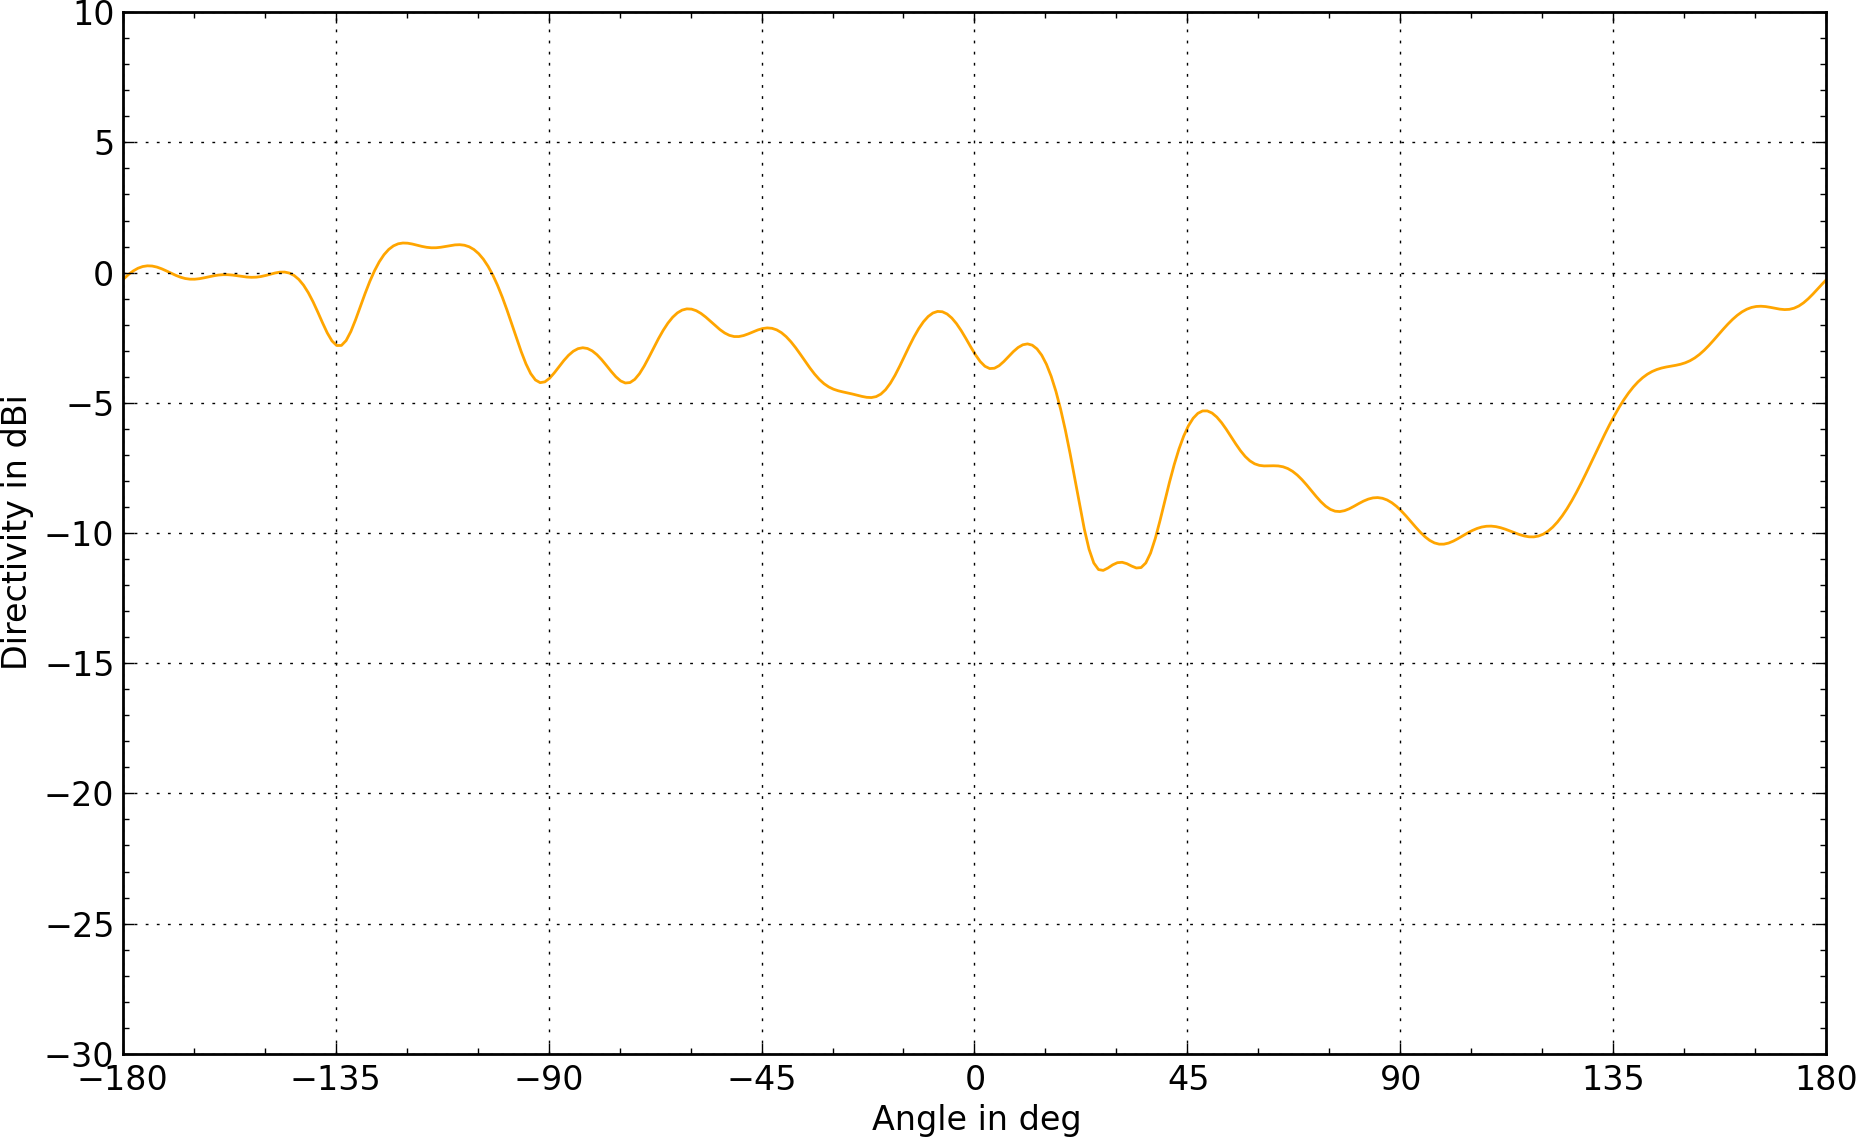
\includegraphics[width=1\textwidth]{../fig/plt/crazy_stuff_l4_pcb_v2c_laptop_1a_105_2ghz4_eabs_phi90-trim.png}
		%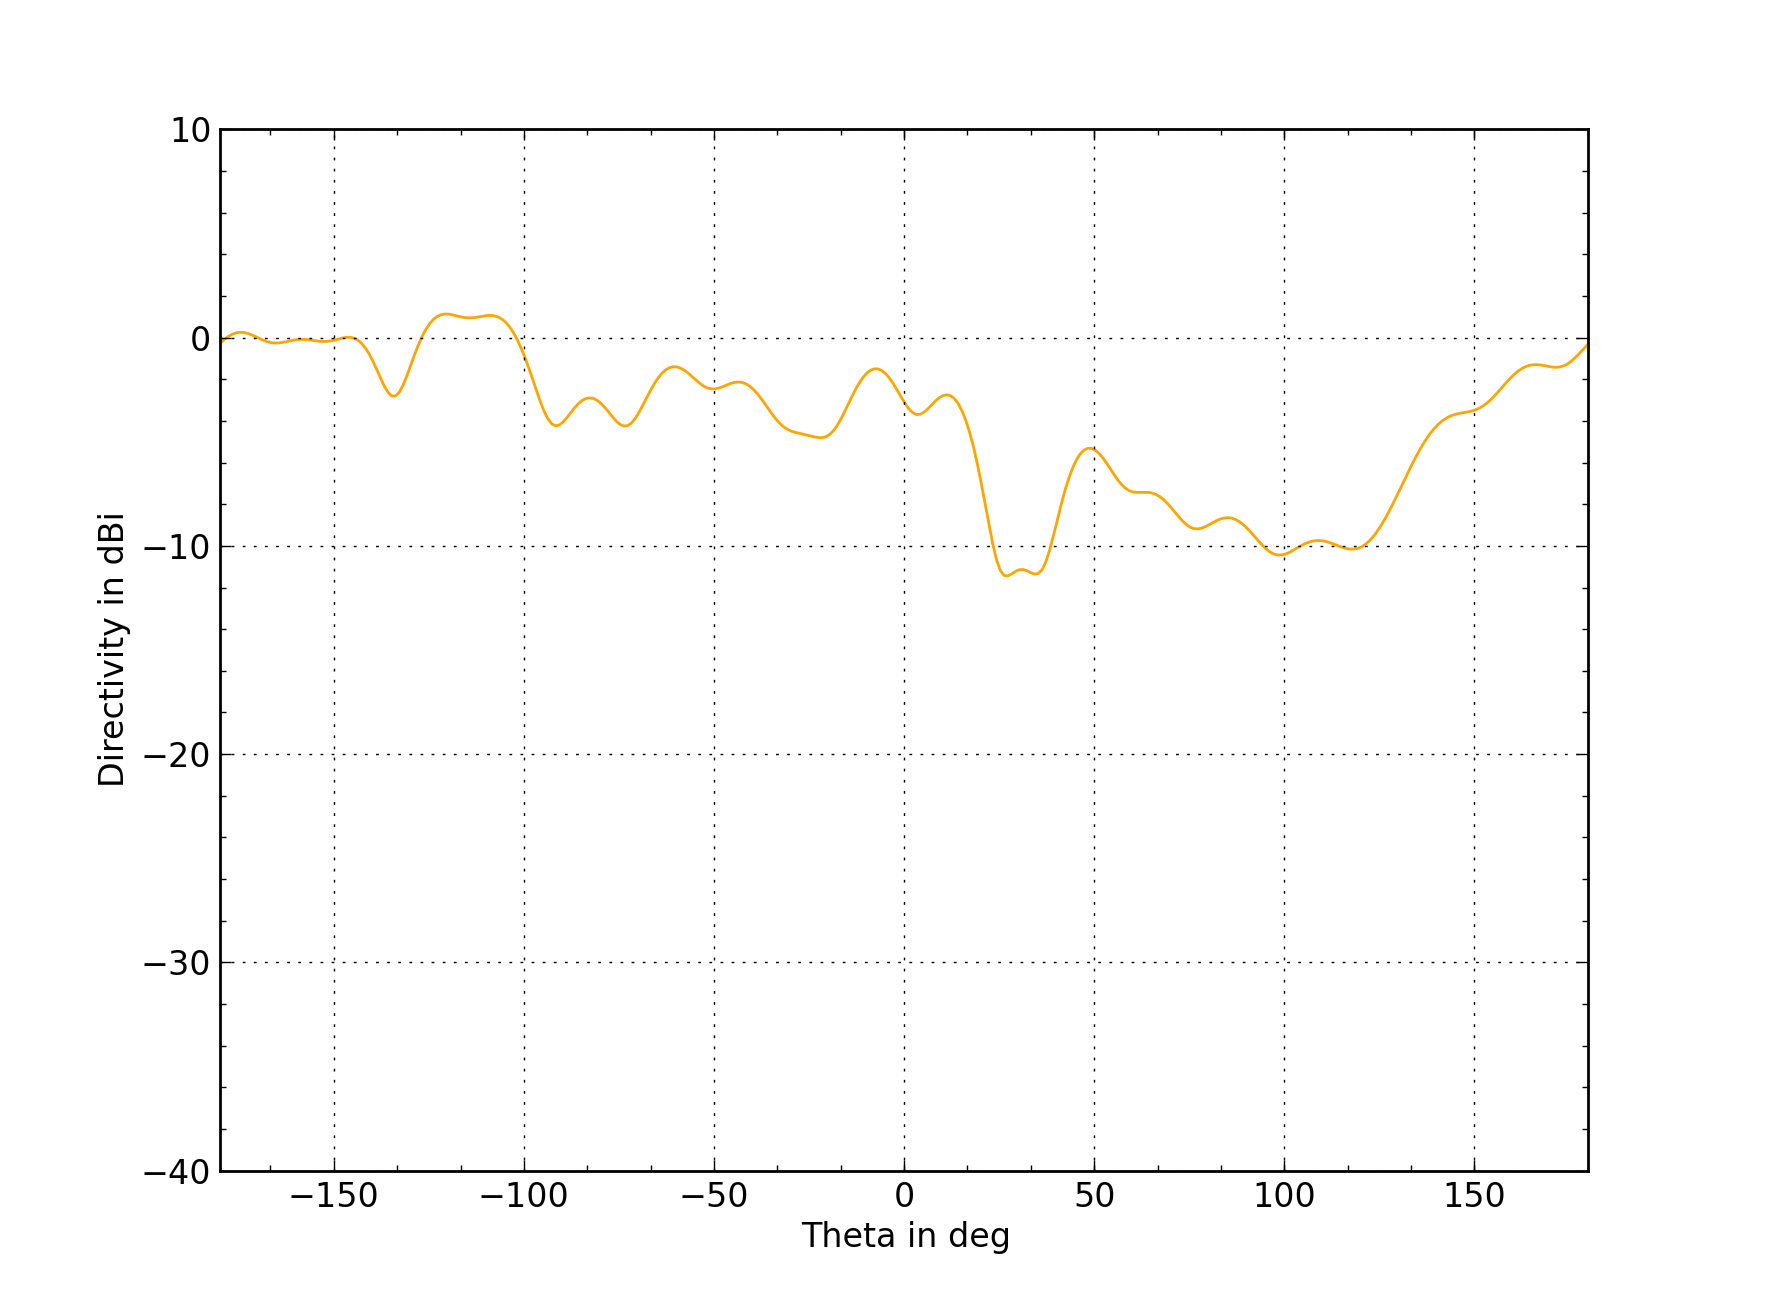
\includegraphics[width=1\textwidth]{../fig/plt/crazy_stuff_l4_pcb_v2c_laptop_1a_105_eabs_phi90_2ghz4.png}
		\caption{Simulation \SI{2.4}{\giga\hertz}}
	\end{subfigure}
	\begin{subfigure}[b]{0.48\textwidth}
		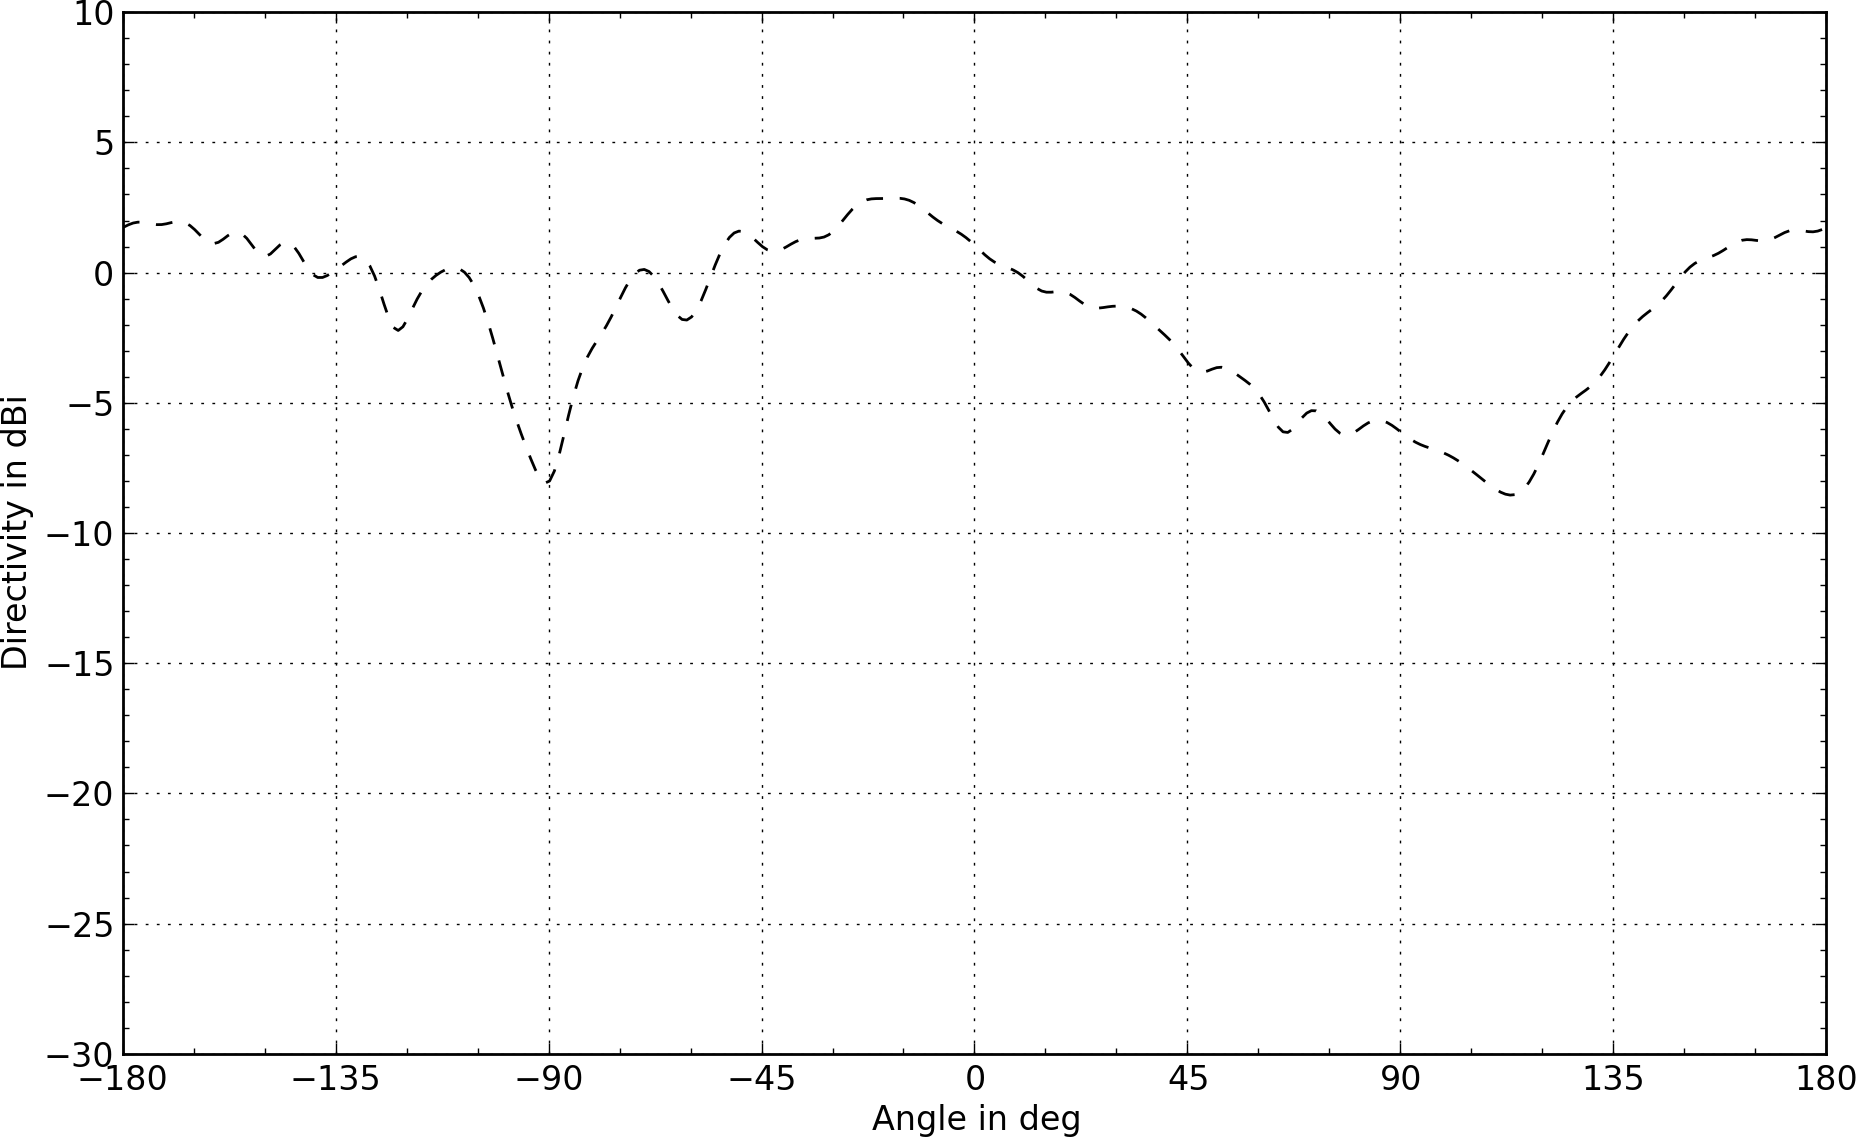
\includegraphics[width=1\textwidth]{../fig/plt/crazy_stuff_l4_pcb_v2c_laptop_1a_105_5ghz0_eabs_phi90-trim.png}
		%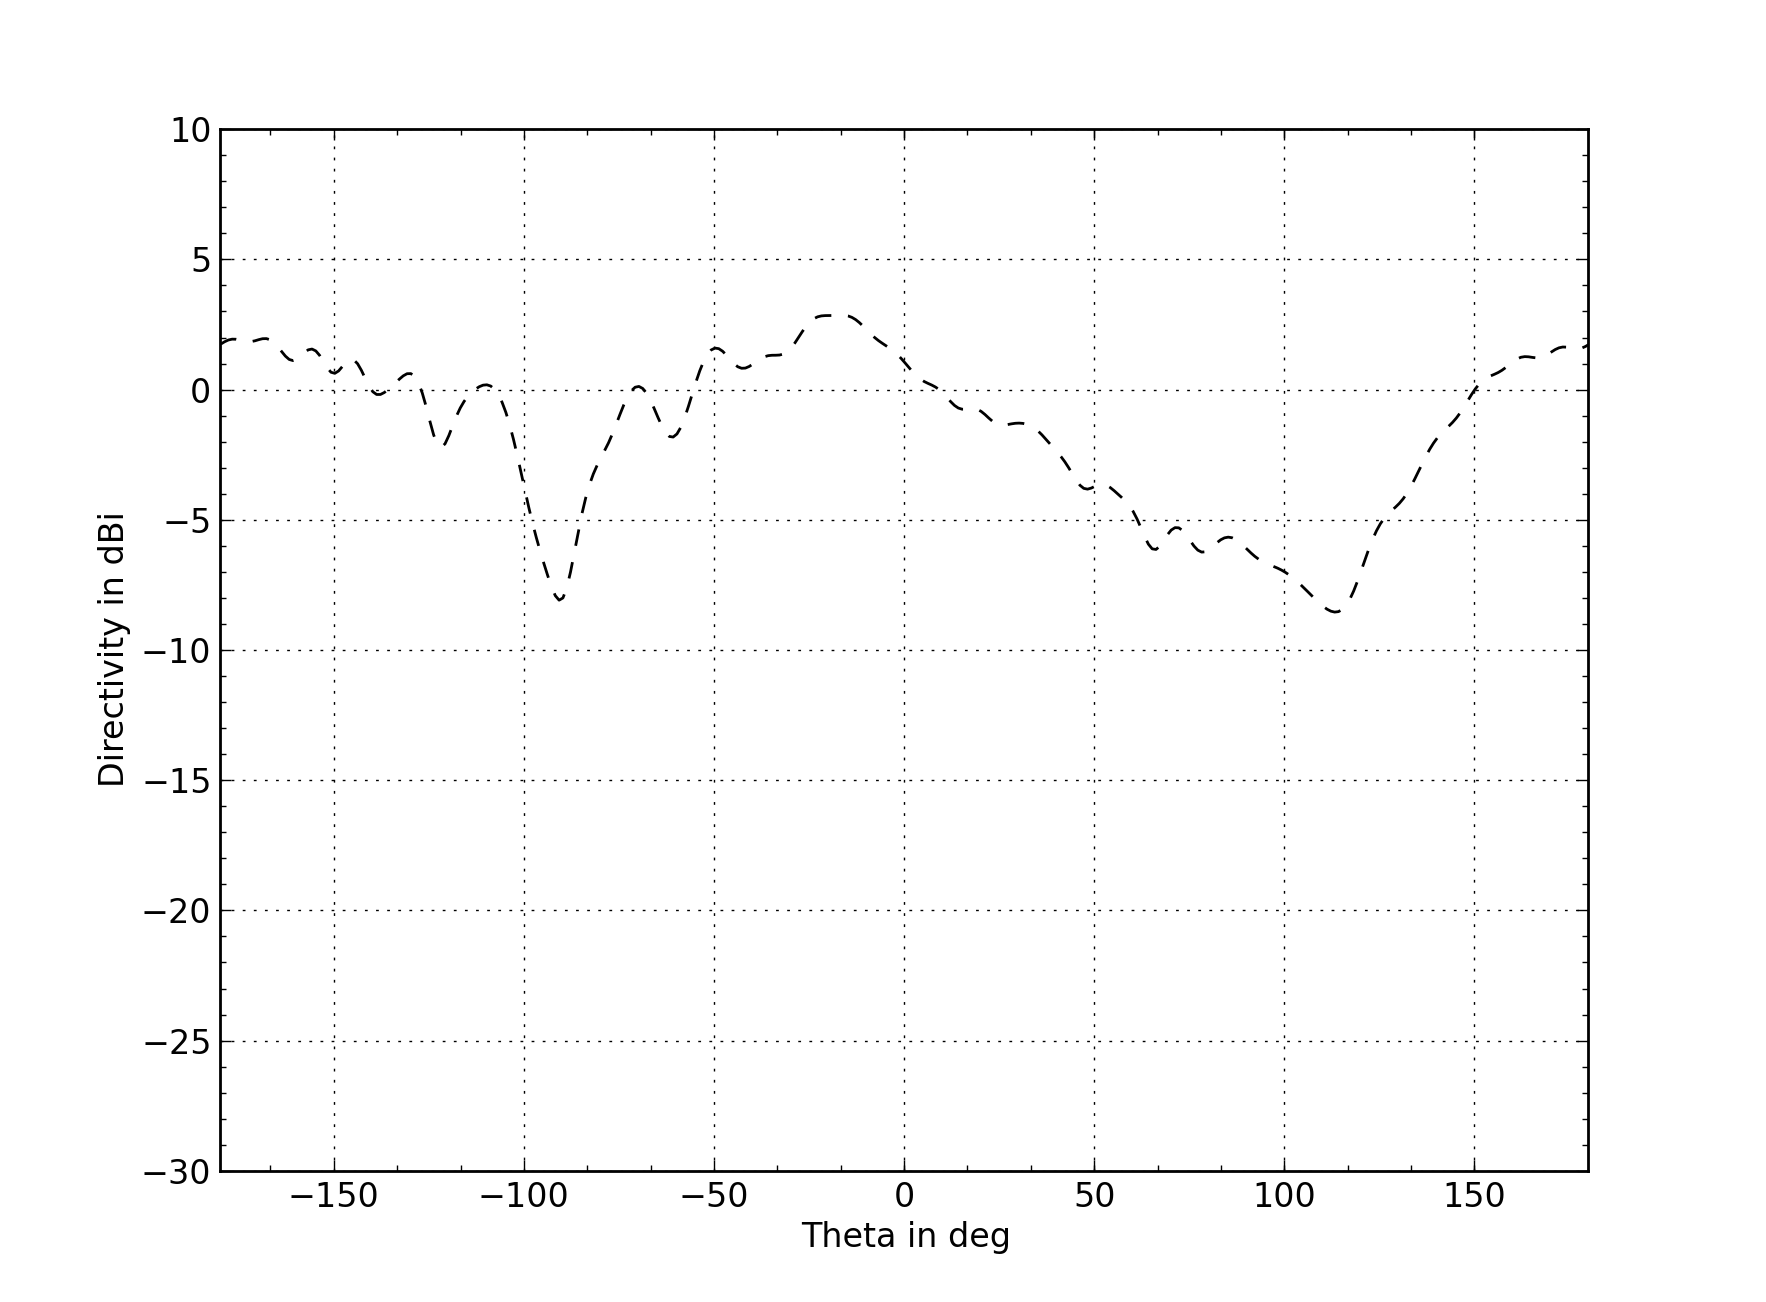
\includegraphics[width=1\textwidth]{../fig/plt/crazy_stuff_l4_pcb_v2c_laptop_1a_105_eabs_phi90_5ghz.png}
		\caption{Simulation \SI{5.0}{\giga\hertz}}
	\end{subfigure}

	\begin{subfigure}[t]{0.49\textwidth}
		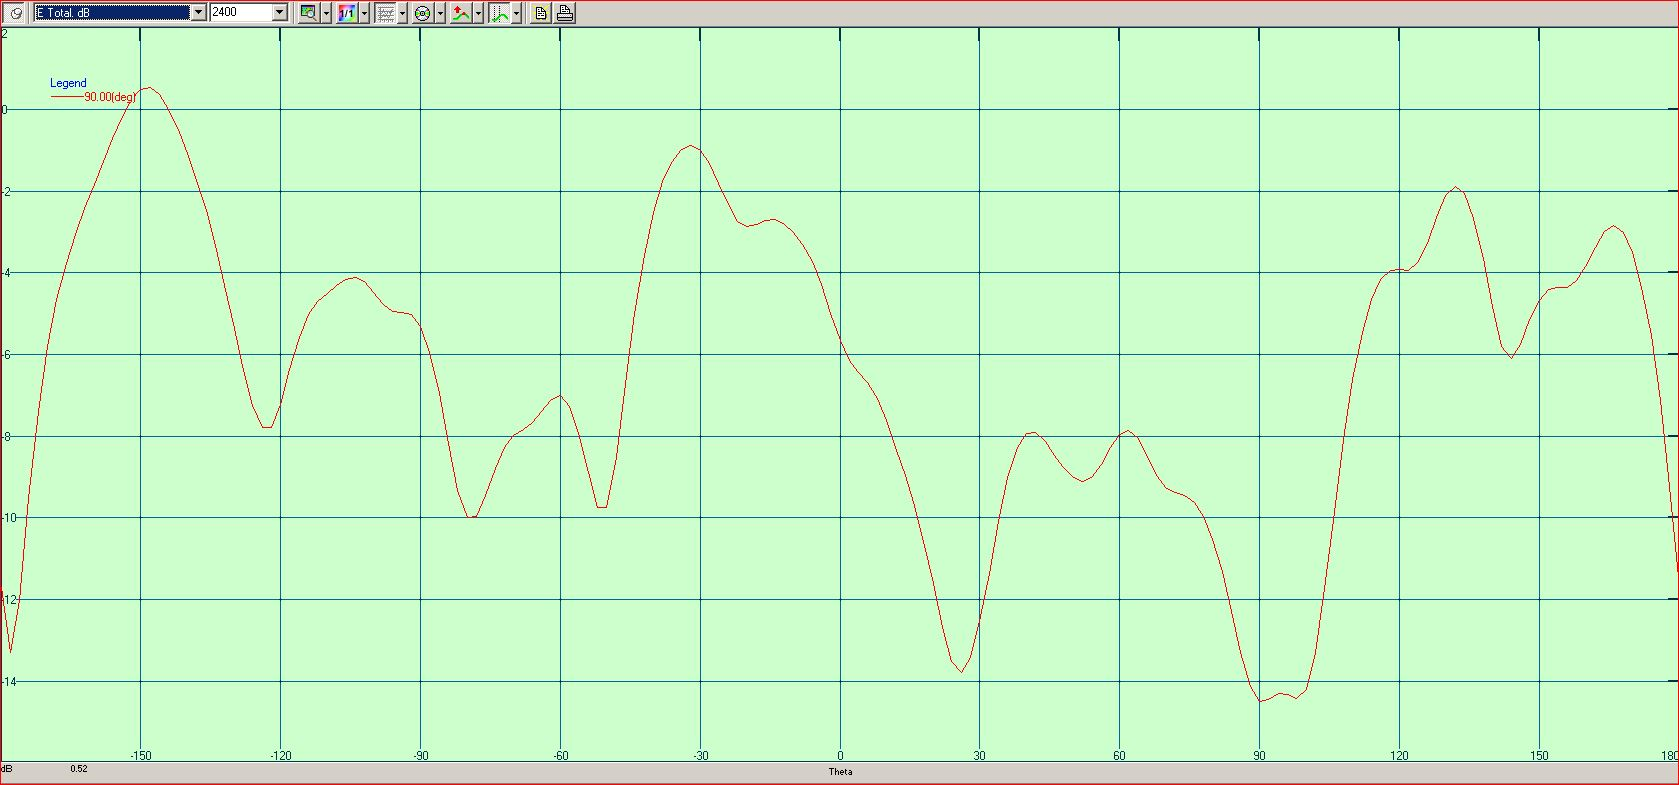
\includegraphics[width=1\textwidth]{../fig/plt/2G4_90phi_etot_dB.JPG}
	 	%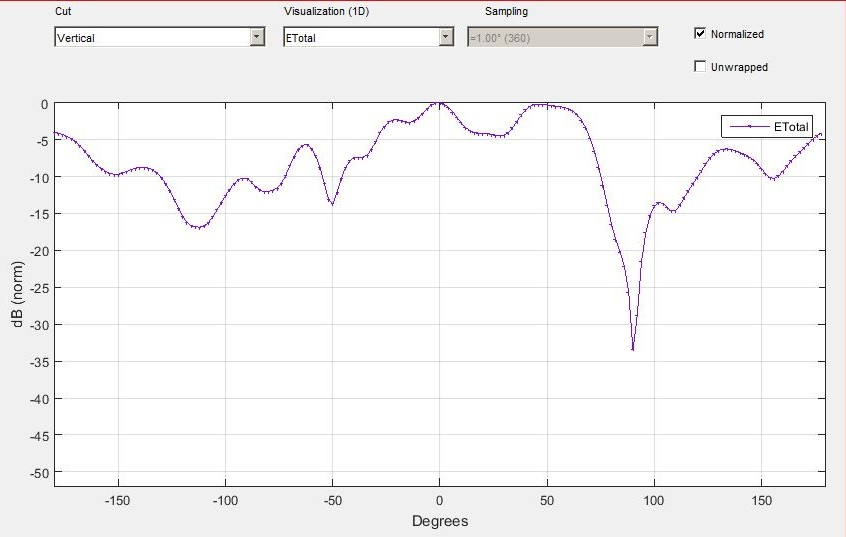
\includegraphics[width=1\textwidth]{../fig/plt/2_4GHz_E_tot_curve.jpg}
		\caption{Messung \SI{2.4}{\giga\hertz}}
	\end{subfigure}
	\begin{subfigure}[t]{0.49\textwidth}
		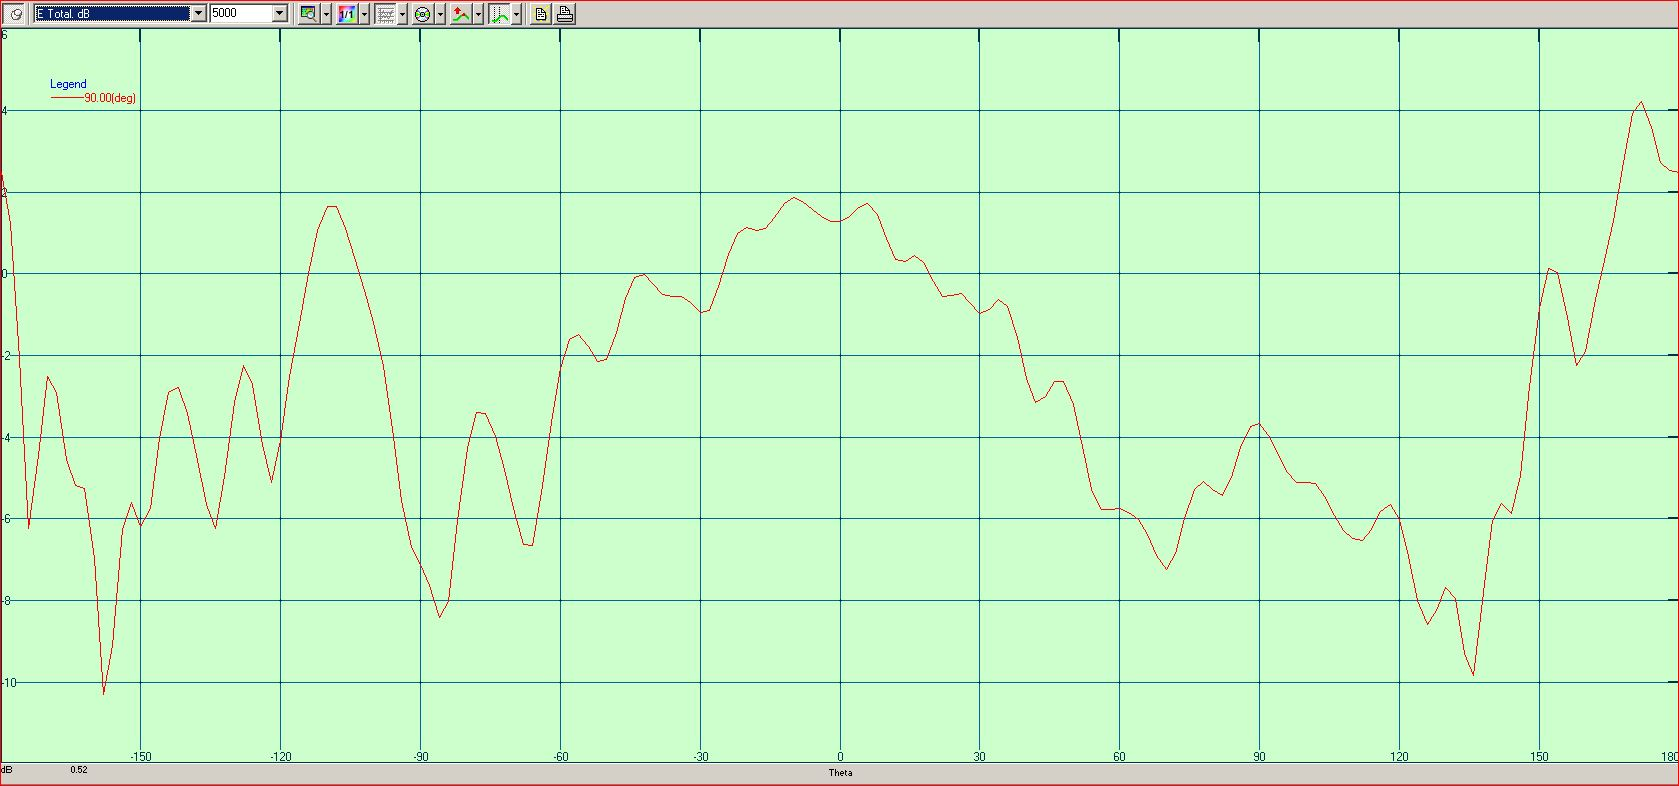
\includegraphics[width=1\textwidth]{../fig/plt/5G0_90phi_etot_dB.JPG}
		%\includegraphics[width=1\textwidth]{../fig/plt/5GHz_E_tot_curve.jpg}
		\caption{Messung \SI{5.0}{\giga\hertz}}
	\end{subfigure}
\end{figure}


 \clearpage
%\section{Fazit}
 \clearpage
\section{Diskussion}

\todo{Die wichtigsten Ergebnisse der Versuche werden in Worte qualitativ
	beschrieben und bewertet. Unstimmigkeiten zwischen den Ergebnissen
	einerseits und den allfällig berechneten / simulierten Grössen
	andererseits sollen diskutiert werden, und mögliche Ursachen als
	Hypothesen formuliert werden.}


%\cite{ts}

% bibliography
%\newpage
%\cleardoublepage
%\addcontentsline{toc}{section}{Literatur}
%% \setlength\bibitemsep{1.5\itemsep}
%\nocite{*}
%\bibliographystyle{apacite}
\bibliographystyle{ieeetr}
%\bibliographystyle{pkg/deIEEEtran}
\bibliography{bib/bibliography}



% glossary
%\newpage
%\cleardoublepage

%\clearpage
%\begin{multicols}{2}
%	\scriptsize
%	\glossarystyle{altlistgroup}
%	\glsaddall
%	\printglossary[title=Glossar]
%	\printglossaries
%\end{multicols}

% list of figures
%\clearpage
%\newpage
%\cleardoublepage
% \phantomsection
%\addcontentsline{toc}{section}{Abbildungen}
%\listoffigures

% lsit of tables
%\clearpage
%\newpage
%\cleardoublepage
% \phantomsection
%\addcontentsline{toc}{section}{Tabellen}
%\listoftables

% appendix
%\clearpage
%\begin{appendices}
%\pagenumbering{roman}
\addtocontents{toc}{\protect\setcounter{tocdepth}{2}}

% appendix contents

%\clearpage

\end{appendices}


	
\end{document}
